\documentclass[12pt]{article}
\usepackage{fullpage}
\usepackage{color}
\usepackage{alltt}
\usepackage{underscore}
\usepackage{environ}
\usepackage{graphicx}
\usepackage{style/fullpage}
\usepackage{style/underscore}
\usepackage{style/environ}
\usepackage{color}
\usepackage{alltt}
\usepackage{graphicx}
\usepackage{etoolbox} % for @for \do ??
\usepackage[hidelinks]{hyperref} % for hyperref
\usepackage{xstring}
\usepackage{adjustbox}

%\IfFileExists{minted.sty}{
%\usepackage{minted}
%\newminted[ccode]{c}{}
%\newminted[cxxcode]{c++}{}
%\newminted[fcode]{fortran}{}
%\newminted[pycode]{python}{}
%\newmint[cfuncsig]{c}{}
%\newmint[cxxfuncsig]{c++}{}
%\newmint[ffuncsig]{fortran}{}
%\newmint[pyfuncsig]{python}{}
%}{
\usepackage{listings}
\lstnewenvironment{ccode}
    {\lstset{language=C, breaklines=true, breakautoindent=true}}
    {}
\lstnewenvironment{cxxcode}
    {\lstset{language=C++, breaklines=true, breakautoindent=true}}
    {}
\lstnewenvironment{fcode}
    {\lstset{language=Fortran, breaklines=true, breakautoindent=true}}
    {}
\lstnewenvironment{pycode}
    {\lstset{language=Python, breaklines=true, breakautoindent=true}}
    {}
%}

\newcommand{\apih}[2]{
\noindent
\section*{#1}
\label{api:#1}
\textit{#2}
}

%\newcommand{\optype}[1]{
%\newline
%\textbf{Operation Type:}#1
%\newline
%}

\newcommand{\wcoll}{
\noindent
\textcolor{blue}{Operation Type:} Collective on the world processor group
\newline
}
\newcommand{\dcoll}{
\noindent
\textcolor{blue}{Operation Type:} Collective on the default processor group
\newline
}
\newcommand{\gcoll}{
\noindent
\textcolor{blue}{Operation Type:} Collective on the processor group inferred from the arguments
\newline
}
\newcommand{\ncoll}{
\noindent
\textcolor{blue}{Operation Type:} One-sided (non-collective)
\newline
}
\newcommand{\local}{
\noindent
\textcolor{blue}{Operation Type:} Local
\newline
}

\newenvironment{desc}{
\noindent
\textcolor{blue}{API description:}\par}{}

\newenvironment{cdesc}{
\noindent
\textcolor{blue}{C API description:}\par}{}

\newenvironment{fdesc}{
\noindent
\textcolor{blue}{Fortran API description:}\par}{}

\newenvironment{cxxdesc}{
\noindent
\textcolor{blue}{C++ API description:}\par}{}

\newenvironment{fapi}{
\noindent
\textcolor{blue}{Fortran Interface}
\small
}{
}

\newenvironment{f2dapi}{
\noindent
\textcolor{blue}{Fortran 2D Interface}
\small
}{
}

\newenvironment{pydesc}{
\noindent
\textcolor{blue}{Python API description:}

}{}

\newenvironment{capi}{
\noindent
\textcolor{blue}{C Interface}
\small
}{
}

\newenvironment{cxxapi}{
\noindent
\textcolor{blue}{C++ Interface}
\small
}{
}

\newenvironment{pyapi}{
\noindent
\textcolor{blue}{Python Interface}
\small
}{
}

\newenvironment{funcargs}{\noindent\begin{tabular}{@{}p{0.16\textwidth}@{}p{0.14\textwidth}@{}p{0.58\textwidth}@{}p{0.08\textwidth}@{}}}{\end{tabular}}

\newcommand{\funcarg}[4]{\texttt{#1}&\texttt{#2}&\texttt{#3}&\texttt{#4}\\}

\newcommand{\inarg}[3]{\texttt{#1}&\texttt{#2}&\texttt{#3}&\textcolor{blue}{\texttt{input}}\\}

\newcommand{\inoutarg}[3]{\texttt{#1}&\texttt{#2}&\texttt{#3}&\texttt{\textcolor{blue}{in}/\textcolor{red}{out}}\\}

\newcommand{\outarg}[3]{\texttt{#1}&\texttt{#2}&\texttt{#3}&\textcolor{red}{\texttt{output}}\\}

\definecolor{copper}{RGB}{213,117,0}
\definecolor{silver}{RGB}{112,114,118}
\definecolor{bronze}{RGB}{168,60,15}
\definecolor{gold}{RGB}{241,171,0}
\definecolor{onyx}{RGB}{36,36,36}
\definecolor{platinum}{RGB}{178,179,181}

\newcounter{SeeAlsoCounter}
\makeatletter
\newcommand*{\seealso}[1]{%
\noindent
\textcolor{blue}{See Also:}
\newline
\def\mystring{#1}
\StrCount{\mystring}{,}[\commacount]
\setcounter{SeeAlsoCounter}{0}
\@for\arg:=#1\do{%
  \hyperref[api:\arg]{\nameref*{api:\arg}}\ifnum\value{SeeAlsoCounter}<\commacount,\fi
  \stepcounter{SeeAlsoCounter}
}%
}
\makeatother

\graphicspath{{./figures/}}

\newenvironment{fapi}{
\noindent
\textcolor{blue}{Fortran Interface}
\begin{alltt} 
\small
\color{red}
}{
\end{alltt}
}

\newenvironment{f2dapi}{
\noindent
\textcolor{blue}{Fortran 2D Interface}
\begin{alltt} 
\small
\color{red}
}{
\end{alltt}
}

\newenvironment{capi}{
\noindent
\textcolor{blue}{C Interface}
\begin{alltt} 
\small
\color{red}
}{
\end{alltt}
\color{black}
}

\newenvironment{cxxapi}{
\noindent
\textcolor{blue}{C++ Interface}
%\vspace{-18pt}
\begin{alltt} 
\small
\color{red}
}{
\end{alltt}
}

\newenvironment{desc}{
\noindent
\textcolor{blue}{API description:}\color{black}}{}




\begin{document}


\apih{INITIALIZE}

\begin{capi}
void NGA_Initialize()
void GA_Initialize()
\end{capi}

\begin{fapi}
subroutine nga_initialize()
subroutine ga_initialize()
\end{fapi}

\begin{cxxapi}
GA::Initialize(int argc, char *argv[], size_t limit)
   argc                  - number of command line arguments              \access{[input]}
   argv                  - command line arguments                        \access{[input]}
   limit                 - amount of memory in bytes per process         \access{[input]}
\end{cxxapi}

\begin{pyapi}
initialize()
\end{pyapi}

\begin{desc}

Allocate and initialize internal data structures in Global Arrays.

This is a collective operation.

\end{desc}


\apih{INITIALIZE_LTD}

\begin{capi}
void GA_Initialize_ltd(size_t limit)
   limit                  - amount of memory in bytes per process         \access{[input]} 
\end{capi}

\begin{fapi}
subroutine ga_initialize_ltd(limit)
   integer limit          - amount of memory in bytes 
                            per process                                   \access{[input]} 
\end{fapi}

\begin{cxxapi}
GA::Initialize(int argc, char *argv[], unsigned long heapSize,
               unsigned long stackSize, int type, size_t limit = 0)
   argc                  - number of command line arguments               \access{[input]}
   argv                  - command line arguments                         \access{[input]}
   limit                 - amount of memory in bytes per process          \access{[input]}
   heapSize, stackSize   - all of the dynamically allocated local memory  \access{[input]}
   type                  - data type                                      \access{[input]}
\end{cxxapi}

\begin{pyapi}
initialize_ltd(size_t limit)
\end{pyapi}

\begin{desc}

  Allocate and initialize internal data structures and set the limit for
  memory used in Global Arrays. The limit is per process: it is the
  amount of memory that the given processor can contribute to
  collective allocation of Global Arrays. It does not include
  temporary storage that GA might be allocating (and releasing) during
  execution of a particular operation.

  $*limit < 0$ means ``allow unlimited memory usage" in which case this
  operation is equivalent to GA_initialize.

This is a collective operation.

\end{desc}


\apih{PGROUP_CREATE}

\begin{capi}
int GA_Pgroup_create(int *list, int size)
   list (size)            - list of processor IDs in group                \access{[input]} 
   size                     number of processors in group                 \access{[input]} 
\end{capi}

\begin{fapi}
integer function ga_pgroup_create(list, size)
   integer       size             - number of processors in group         \access{[input]} 
   integer       list (size)      - list of processors in 
                                    processor group                       \access{[input]} 
\end{fapi}

\begin{cxxapi}
PGroup::PGroup(int *plist, int size)
   size                              - number of processors in group      \access{[input]}
   plist[size]                       - list of processor IDs in group     \access{[input]}
\end{cxxapi}

\begin{pyapi}
pgroup_create(list)
\end{pyapi}

\begin{desc}

  This command is used to create a processor group. At present, it
  must be invoked by all processors in the current default processor
  group. The list of processors use the indexing scheme of the default
  processor group. If the default processor group is the world group,
  then these indices are the usual processor indices. This function
  returns a process group handle that can be used to reference this
  group by other functions.

  This is a collective operation on the default processor group.

\end{desc}


\apih{PGROUP_DESTROY}

\begin{capi}
int GA_Pgroup_destroy(int p_handle)
   p_handle               - processor group handle                        \access{[input]} 
\end{capi}

\begin{fapi}
logical function ga_pgroup_destroy(p_handle)
   integer      p_handle          - processor group handle                \access{[input]} 
\end{fapi}

\begin{cxxapi}
PGroup::~PGroup()
\end{cxxapi}

\begin{pyapi}
pgroup_destroy(int pgroup)
\end{pyapi}

\begin{desc}

  This command is used to free up a processor group handle. It returns
  0 if the processor group handle was not previously active.

  This is a collective operation on the default processor group.

\end{desc}

\apih{PGROUP_SET_DEFAULT}

\begin{capi}
void GA_Pgroup_set_default(int p_handle)
   p_handle               - processor group handle                        \access{[input]} 
\end{capi}

\begin{fapi}
subroutine ga_pgroup_set_default(p_handle)
   integer     p_handle           - processor group handle                \access{[input]} 
\end{fapi}

\begin{cxxapi}
static void PGroup::setDefault(PGroup *p_handle)
  p_handle                - processor group                               \access{[input]}
\end{cxxapi}

\begin{pyapi}
pgroup_set_default(int pgroup)
\end{pyapi}

\begin{desc}

  This function can be used to reset the default processor group on a
  collection of processors. All processors in the group referenced by
  p_handle must make a call to this function. Any standard global
  array call that is made after resetting the default processor group
  will be restricted to processors in that group. Global arrays that
  are created after resetting the default processor group will only be
  defined on that group and global operations, such as GA_Sync or
  GA_Igop, and will be restricted to processors in that group. The
  GA_Pgroup_set_default call can be used to rapidly convert large
  applications, written with GA, into routines that run on processor
  groups.

  The default processor group can be overridden by using GA calls that
  require an explicit group handle as one of the arguments.

  This is a collective operation on the group represented by the
  handle p_handle.

\end{desc}

\apih{CREATE}

\begin{capi}
int NGA_Create(int type, int ndim, int dims[], char *array_name, int 
               chunk[])
   array_name             - a unique character string                     \access{[input]} 
   type                   - data type (MT_F_DBL,MT_F_INT,MT_F_DCPL)       \access{[input]} 
   ndim                   - number of array dimensions                    \access{[input]} 
   dims[ndim]             - array of dimensions                           \access{[input]} 
   chunk[ndim]            - array of chunks, each element specifies 
                            minimum size that given dimensions should 
                            be chunked up into                            \access{[input]} 
\end{capi}

\begin{f2dapi}
logical function ga_create(type, dim1, dim2, array_name, chunk1, 
                           chunk2, g_a)
   character*(*) array_name        - a unique character string            \access{[input]} 
   integer       type              - MA type                              \access{[input]} 
   integer       dim1/2            - array (dim1,dim2) as in FORTRAN      \access{[input]} 
   integer       chunk1/2          - minimum size that dimensions should
                                     be chunked up into                   \access{[input]} 
   integer       g_a               - handle for future references         \access{[output]} 
\end{f2dapi}

\begin{fapi}
logical function nga_create(type, ndim, dims, array_name, chunk, g_a)
   character*(*) array_name        - a unique character string            \access{[input]} 
   integer       type              - data type (MT_DBL,MT_INT,MT_DCPL)    \access{[input]} 
   integer       ndim              - number of array dimensions           \access{[input]} 
   integer       dims(ndim)        - array of dimensions                  \access{[input]} 
   integer       chunk(ndim)       - array of chunks, each element specifies
                                     minimum size that given dimensions
                                     should be chunked up into            \access{[input]} 
   integer       g_a               - integer handle for future references \access{[output]} 
\end{fapi}

\begin{cxxapi}
GlobalArray::GlobalArray* createGA(int type, int ndim, int dims[],
                                   char *arrayname, int chunk[])
GlobalArray * GAServices::createGA(int type, int ndim, int dims[],
                                           char *arrayname, int chunk[])
   type             - data type(MT_F_DBL,MT_F_INT,MT_F_DCPL)              \access{[input]}
   ndim             - number of array dimensions                          \access{[input]}
   dims[ndim]       - array of dimensions                                 \access{[input]}
   arrayname        - a unique character string                           \access{[input]}
   chunk[ndim]      - array of chunks, each element specifies
                      minimum size that given dimensions should be
                      chunked up into                                     \access{[input]}
\end{cxxapi}

\begin{pyapi}
create(int gtype, dims, char *name='', chunk=None, int pgroup=-1)
   gtype (int) - the type of the array
   dims (1D array-like of integers) - shape of the array
   name (string) - the name of the array
   chunk (1D array-like of integers) - see above
   pgroup (int) - create array only as part of this processor group
\end{pyapi}

\begin{desc}

  Creates an ndim-dimensional array using the regular distribution
  model and returns an integer handle representing the array.

  The array can be distributed evenly or not. The control over the
  distribution is accomplished by specifying chunk (block) size for
  all or some of array dimensions. For example, for a 2-dimensional
  array, setting chunk[0]=dim[0] gives distribution by vertical strips
  (chunk[0]*dims[0]); setting chunk[1]=dim[1] gives distribution by
  horizontal strips (chunk[1]*dims[1]). Actual chunks will be modified
  so that they are at least the size of the minimum and each process
  has either zero or one chunk. Specifying chunk[i] as less than 1 will cause
  that dimension to be distributed evenly.

  As a convenience, when chunk is specified as NULL, the entire array
  is distributed evenly.

  Return value: a non-zero array handle means the call was succesful.
  This is a collective operation.
\end{desc}


\apih{CREATE_CONFIG}

\begin{capi}
int NGA_Create_config(int type, int ndim, int dims[], char *array_name,
                      int chunk[], int p_handle)
   array_name             - a unique character string                     \access{[input]} 
   type                   - data type (MT_F_DBL,MT_F_INT,MT_F_DCPL)       \access{[input]} 
   ndim                   - number of array dimensions                    \access{[input]} 
   dims[ndim]             - array of dimensions                           \access{[input]} 
   chunk[ndim]            - array of chunks, each element specifies
                            minimum size that given dimensions should
                            be chunked up into                            \access{[input]} 
   p_handle               - processor list handle                         \access{[input]} 
\end{capi}

\begin{fapi}
logical function nga_create_config(type, ndim, dims, array_name, chunk,
                                   p_handle, g_a)
   character*(*) array_name       - a unique character string             \access{[input]} 
   integer       type             - data type (MT_DBL,MT_INT,MT_DCPL)     \access{[input]} 
   integer       ndim             - number of array dimensions            \access{[input]} 
   integer       dims(ndim)       - array of dimensions                   \access{[input]} 
   integer       chunk(ndim)      - array of chunks, each element specifies
                                    minimum size that given dimensions
                                    should be chunked up into             \access{[input]} 
   integer       p_handle         - processor group handle                \access{[input]} 
   integer       g_a              - integer handle for future references  \access{[output]} 
\end{fapi}

\begin{cxxapi}
GlobalArray::GlobalArray(int type, int ndim, int dims[], char *arrayname,
                         int chunk[],PGroup* p_handle)
GlobalArray::GlobalArray(int type, int ndim, int64_t dims[], char *arrayname,
                         int64_t chunk[], PGroup* p_handle)
   type             - data type(MT_F_DBL,MT_F_INT,MT_F_DCPL)              \access{[input]}
   ndim             - number of array dimensions                          \access{[input]}
   dims[ndim]       - array of dimensions                                 \access{[input]}
   arrayname        - a unique character string                           \access{[input]}
   chunk[ndim]      - array of chunks, each element specifies
                      minimum size that given dimensions should be
                      chunked up into                                     \access{[input]}
   p_handle         - processor group handle                              \access{[input]}
\end{cxxapi}

\begin{desc}

  Creates an ndim-dimensional array using the regular distribution
  model but with an explicitly specified processor list handle and
  returns an integer handle representing the array.

  This call is essentially the same as the NGA_Create call, except for
  the processor list handle p_handle. It can be used to create
  mirrored arrays.

  Return value: a non-zero array handle means the call was succesful.
  This is a collective operation.

\end{desc}

\apih{CREATE_GHOSTS}

\begin{capi}
int NGA_Create_ghosts(int type, int ndim, int dims[], int width[],
                      char *array_name, int chunk[])
   array_name             - a unique character string                     \access{[input]} 
   type                   - data type (MT_DBL,MT_INT,MT_DCPL)             \access{[input]} 
   ndim                   - number of array dimensions                    \access{[input]} 
   dims[ndim]             - array of dimensions                           \access{[input]} 
   width[ndim]            - array of ghost cell widths                    \access{[input]} 
   chunk[ndim]            - array of chunks, each element specifies
                            minimum size that given dimensions should
                            be chunked up into                            \access{[input]} 
\end{capi}

\begin{fapi}
logical function nga_create_ghosts(type, ndim, dims, width, array_name, 
                                   chunk, g_a) 
   character*(*) array_name       - a unique character string             \access{[input]} 
   integer       type             - data type (MT_DBL,MT_INT,MT_DCPL)     \access{[input]} 
   integer       ndim             - number of array dimensions            \access{[input]} 
   integer       dims(ndim)       - array of dimensions                   \access{[input]} 
   integer       width(ndim)      - array of ghost cell widths            \access{[input]} 
   integer       chunk(ndim)      - array of chunks, each element specifies
                                    minimum size that given dimensions
                                    should be chunked up into             \access{[input]} 
   integer       g_a              - integer handle for future references  \access{[output]} 
\end{fapi}

\begin{cxxapi}
GlobalArray::GlobalArray(int type, int ndim, int dims[], int width[],
                         char *arrayname, int chunk[], char ghosts)
GlobalArray::GlobalArray(int type, int ndim, int64_t dims[], int64_t width[],
                         char *arrayname, int64_t chunk[], char ghosts)
GlobalArray * GAServices::createGA_Ghosts(int type, int ndim, int dims[],
                                          int width[], char *array_name, 
                                          int chunk[])
   type             - data type (MT_DBL,MT_INT,MT_DCPL)                   \access{[input]}
   ndim             - number of array dimensions                          \access{[input]}
   dims[ndim]       - array of dimensions                                 \access{[input]}
   width[ndim]      - array of ghost cell widths                          \access{[input]}
   array_name       - a unique character string                           \access{[input]}
   chunk[ndim]      - array of chunks, each element specifies
                      minimum size that given dimensions should be
                      chunked up into                                     \access{[input]}
   ghosts           - this is a dummy parameter: added to increase the
                      number of arguments, in order to avoid the conflicts
                      among constructors. (ghosts = 'g' or 'G')           \access{[input]}
\end{cxxapi}

\begin{pyapi}
create_ghosts(int gtype, dims, width, char *name='', chunk=None, int pgroup=-1)
   gtype (int)                       - the type of the array
   dims (1D array-like of integers)  - shape of the array
   width (1D array-like of integers) - ghost cell widths
   name (string)                     - the name of the array
   chunk (1D array-like of integers) - see above
   pgroup (int)                      - create array only as part of this 
                                       processor group
\end{pyapi}

\begin{desc}

  Creates an ndim-dimensional array with a layer of ghost cells around
  the visible data on each processor using the regular distribution
  model and returns an integer handle representing the array.

  The array can be distributed evenly or not evenly. The control over
  the distribution is accomplished by specifying chunk (block) size
  for all or some of the array dimensions. For example, for a
  2-dimensional array, setting chunk(1)=dim(1) gives distribution by
  vertical strips (chunk(1)*dims(1)); setting chunk(2)=dim(2) gives
  distribution by horizontal strips (chunk(2)*dims(2)). Actual chunks
  will be modified so that they are at least the size of the minimum
  and each process has either zero or one chunk. Specifying chunk(i)
  as \textless 1 will cause that dimension (i-th) to be distributed evenly. The
  width of the ghost cell layer in each dimension is specified using
  the array width(). The local data of the global array residing on
  each processor will have a layer width[n] ghosts cells wide on
  either side of the visible data along the dimension n.

  Return value: a non-zero array handle means the call was successful.

  This is a collective operation.
\end{desc}


\apih{CREATE_GHOSTS_CONFIG}

\begin{capi}
int NGA_Create_ghosts_config(int type, int ndim, int dims[], 
                             int width[], char *array_name, int chunk[], 
                             int p_handle)
   array_name             - a unique character string                     \access{[input]} 
   type                   - data type (MT_DBL,MT_INT,MT_DCPL)             \access{[input]} 
   ndim                   - number of array dimensions                    \access{[input]} 
   dims[ndim]             - array of dimensions                           \access{[input]} 
   width[ndim]            - array of ghost cell widths                    \access{[input]} 
   chunk[ndim]            - array of chunks, each element specifies
                            minimum size that given dimensions should be
                            chunked up into                               \access{[input]} 
   p_handle               - processor list handle
\end{capi}

\begin{fapi}
logical function nga_create_ghosts_config(type, ndim, dims, width, 
                                          array_name, chunk, p_handle, g_a)
   character*(*) array_name       - a unique character string             \access{[input]} 
   integer       type             - data type (MT_DBL,MT_INT,MT_DCPL)     \access{[input]} 
   integer       ndim             - number of array dimensions            \access{[input]} 
   integer       dims(ndim)       - array of dimensions                   \access{[input]} 
   integer       width(ndim)      - array of ghost cell widths            \access{[input]} 
   integer       chunk(ndim)      - array of chunks, each element specifies
                                    minimum size that given dimensions
                                    should be chunked up into             \access{[input]} 
   integer       p_handle         - processor group handle                \access{[input]} 
   integer       g_a              - integer handle for future references  \access{[output]} 
\end{fapi}

\begin{cxxapi}
GlobalArray::GlobalArray(int type, int ndim, int dims[], int width[], 
                         char *arrayname, int chunk[], PGroup* p_handle, 
                         char ghosts)
GlobalArray::GlobalArray(int type, int ndim, int64_t dims[], int64_t width[],
                         char *arrayname, int64_t chunk[], PGroup* p_handle, 
                         char ghosts)
   type             - data type (MT_DBL,MT_INT,MT_DCPL)                   \access{[input]}
   ndim             - number of array dimensions                          \access{[input]}
   dims[ndim]       - array of dimensions                                 \access{[input]}
   width[ndim]      - array of ghost cell widths                          \access{[input]}
   array_name       - a unique character string                           \access{[input]}
   chunk[ndim]      - array of chunks, each element specifies
                      minimum size that given dimensions should be
                      chunked up into                                     \access{[input]}
   p_handle         - processor group handle                              \access{[input]}
   ghosts           - this is a dummy parameter: added to increase the
                      number of arguments, inorder to avoid the conflicts
                      among constructors. (ghosts = 'g' or 'G')           \access{[input]}
\end{cxxapi}

\begin{desc}

  Creates an ndim-dimensional array with a layer of ghost cells around
  the visible data on each processor using the regular distribution
  model and an explicitly specified processor list and returns an
  integer handle representing the array.

  This call is essentially the same as the NGA_Create_ghosts call,
  except for the processor list handle p_handle. It can be used to
  create mirrored arrays.

  Return value: a non-zero array handle means the call was successful.
  This is a collective operation.

\end{desc}

\apih{CREATE_IRREG}

\begin{capi}
int NGA_Create_irreg(int type, int ndim, int dims[], char *array_name, 
                     int block[], int map[])
   array_name             - a unique character string                     \access{[input]} 
   type                   - MA data type (MT_F_DBL,MT_F_INT,MT_F_DCPL)    \access{[input]}        
   ndim                   - number of array dimensions                    \access{[input]} 
   dims                   - array of dimension values                     \access{[input]} 
   nblock[ndim]           - no. of blocks each dimension is divided into  \access{[input]} 
   map[s]                 - starting index for for each block; the size
                            s is a sum all elements of nblock array       \access{[input]} 
\end{capi}

\begin{f2dapi}
logical function ga_create_irreg(type, dim1, dim2, array_name, map1, 
                                 nblock1, map2, nblock2, g_a)
    character*(*) array_name      - a unique character string             \access{[input]} 
    integer type                  - MA type                               \access{[input]} 
    integer dim1/2                - array (dim1,dim2) as in FORTRAN       \access{[input]} 
    integer nblock1               - no. of blocks first dimension is
                                    divided into                          \access{[input]} 
    integer nblock2               - no. of blocks second dimension is
                                    divided into                          \access{[input]} 
    integer map1(*)               - ilo for each block                    \access{[input]} 
    integer map2(*)               - jlo for each block                    \access{[input]} 
    integer g_a                   - integer handle for future references  \access{[output]} 
\end{f2dapi}

\begin{fapi}
logical function nga_create_irreg(type, ndim, dims, array_name, map, 
                                  nblock, g_a)
   character*(*) array_name       - a unique character string             \access{[input]} 
   integer       type             - data type (MT_DBL,MT_INT,MT_DCPL)     \access{[input]} 
   integer       ndim             - number of array dimensions            \access{[input]} 
   integer       dims(ndim)       - array of dimensions                   \access{[input]} 
   integer       nblock(ndim)     - no. of blocks each dimension is
                                    divided into                          \access{[input]} 
   integer       map(s)           - starting index for for each block; 
                                    the size s is a sum of all elements
                                    of nblock array                       \access{[input]} 
   integer       g_a              - integer handle for future references  \access{[output]} 
\end{fapi}

\begin{cxxapi}
GlobalArray * GAServices::createGA(int type, int ndim, int dims[], 
                                   char *arrayname,
                                   int block[], int maps[])
GlobalArray::GlobalArray(int type, int ndim, int dims[], char *arrayname,
                         int block[],int maps[]);
GlobalArray::GlobalArray(int type, int ndim, int64_t dims[], 
                         char *arrayname, int64_t block[], 
                         int64_t maps[])
   type            - MA data type (MT_F_DBL,MT_F_INT,MT_F_DCPL)          \access{[input]}
   ndim            - number of array dimensions                          \access{[input]}
   dims            - array of dimension values                           \access{[input]}
   arrayname       - a unique character string                           \access{[input]}
   block[ndim]     - no. of blocks each dimension is divided into        \access{[input]}
   maps[s]         - starting index for for each block;
                     the size s is a sum all elements of nblock array    \access{[input]}
\end{cxxapi}

\begin{pyapi}
create_irreg(int gtype, dims, block, map, char *name='', int pgroup=-1)
   gtype (int)                       - the type of the array
   dims (1D array-like of integers)  - shape of the array
   block (1D array-like of integers) - the number of blocks each dimension 
                                       is divided into
   map (1D array-like of integers)   - starting index for each block 
                                       len(map) == sum of all elements of 
                                       nblock array
   name (string)                     - the name of the array
   pgroup (int)                      - create array only as part of this 
                                       processor group
\end{pyapi}

\begin{desc}

  Creates an array by following the user-specified distribution and
  returns an integer handle representing the array.

  The distribution is specified as a Cartesian product of
  distributions for each dimension. The array indices start at 0. 
For example, Figure \ref{crirreg} demonstrates the distribution of a 2-dimensional 8x10 array on 6 (or more) processors.  

nblock[2]=\{3,2\}, the size of the map array is s=5 and the array map contains the following 

  elements map=\{0,2,6, 0, 5\}. The distribution is nonuniform because
  P1 and P4 get 20 elements each and processors P0, P2, P3, and P5 only
  10 elements each.


\begin{figure}
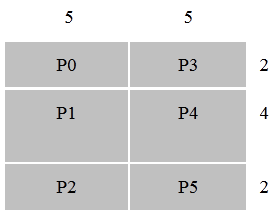
\includegraphics{CrIrreg}
\centering
\caption{Creating an Irregular Array}
\label{crirreg}
\end{figure}
 
  Return value: a non-zero array handle means the call was succesful.
  This is a collective operation.

\end{desc}


\apih{CREATE_IRREG_CONFIG}

\begin{capi}
int NGA_Create_irreg_config(int type, int ndim, int dims[], 
                            char *array_name, int block[], int map[], 
                            int p_handle)
   array_name             - a unique character string                     \access{[input]} 
   type                   - MA data type (MT_F_DBL,MT_F_INT,MT_F_DCPL)    \access{[input]}        
   ndim                   - number of array dimensions                    \access{[input]} 
   dims                   - array of dimension values                     \access{[input]} 
   nblock[ndim]           - no. of blocks each dimension is 
                            divided into                                  \access{[input]} 
   map[s]                 - starting index for for each block; the size
                            s is a sum all elements of nblock array       \access{[input]} 
   p_handle               - processor list handle
\end{capi}

\begin{fapi}
logical function nga_create_irreg_config(type, ndim, dims, 
                                         array_name, map, nblock, 
                                         p_handle, g_a)
   character*(*) array_name       - a unique character string             \access{[input]} 
   integer       type             - data type (MT_DBL,MT_INT,MT_DCPL)     \access{[input]} 
   integer       ndim             - number of array dimensions            \access{[input]} 
   integer       dims(ndim)       - array of dimensions                   \access{[input]} 
   integer       nblock(ndim)     - no. of blocks each dimension is
                                    divided into                          \access{[input]} 
   integer       map(s)           - starting index for for each block;
                                    the size s is a sum of all elements
                                    of nblock array                       \access{[input]} 
   integer       p_handle         - processor group handle                \access{[input]} 
   integer       g_a              - integer handle for future 
                                    references                            \access{[output]} 
\end{fapi}

\begin{cxxapi}
GlobalArray::  GlobalArray(int type, int ndim, int dims[], 
                           char *arrayname, int block[],
                           int maps[], PGroup* p_handle)
GlobalArray::  GlobalArray(int type, int ndim, int64_t dims[], 
                           char *arrayname,
                           int64_t block[], int64_t maps[], 
                           PGroup* p_handle)
   type            - MA data type (MT_F_DBL,MT_F_INT,MT_F_DCPL)          \access{[input]}
   ndim            - number of array dimensions                          \access{[input]}
   dims            - array of dimension values                           \access{[input]}
   arrayname       - a unique character string                           \access{[input]}
   block[ndim]     - no. of blocks each dimension is divided into        \access{[input]}
   maps[s]         - starting index for for each block;
                     the size s is a sum all elements of nblock array    \access{[input]}
   p_handle        - processor group handle                              \access{[input]}
\end{cxxapi}

\begin{desc}

  Creates an array by following the user-specified distribution and an
  explicitly specified processor list handle and returns an integer
  handle representing the array.

  This call is essentially the same as the NGA_Create_irreg call,
  except for the processor list handle p_handle. It can be used to
  create mirrored arrays.

  Return value: a non-zero array handle means the call was succesful.
  This is a collective operation.

\end{desc}


\apih{CREATE_GHOST_IRREG}

\begin{capi}
int NGA_Create_ghost_irreg(int type, int ndim, int dims[], width[],
                           char *array_name, nblock[], map[])
   array_name            - a unique character string                      \access{[input]} 
   type                  - data type (MT_DBL,MT_INT,MT_DCPL)              \access{[input]} 
   ndim                  - number of array dimensions                     \access{[input]} 
   dims[ndim]            - array of dimensions                            \access{[input]} 
   width[ndim]           - array of ghost cell widths                     \access{[input]} 
   nblock[ndim]          - no. of blocks each dimension is 
                           divided into                                   \access{[input]} 
   map[s]                - starting index for for each block; the size     
                           s is a sum of all elements of nblock array     \access{[input]} 
\end{capi}

\begin{fapi}
logical function nga_create_ghosts_irreg(type, ndim, dims, width, 
                                         array_name, map, nblock, g_a)
   character*(*) array_name       - a unique character string             \access{[input]} 
   integer       type             - data type (MT_DBL,MT_INT,MT_DCPL)     \access{[input]} 
   integer       ndim             - number of array dimensions            \access{[input]} 
   integer       dims(ndim)       - array of dimensions                   \access{[input]} 
   integer       width(ndim)      - array of ghost cell widths            \access{[input]} 
   integer       nblock(ndim)     - no. of blocks each dimension is
                                    divided into                          \access{[input]} 
   integer       map(s)           - starting index for for each block; 
                                    the size s is a sum of all elements
                                    of nblock array                       \access{[input]} 
   integer       g_a              - integer handle for future 
                                    references                            \access{[output]} 
\end{fapi}

\begin{cxxapi}
GlobalArray::GlobalArray(int type, int ndim, int dims[], int width[], 
                         char *arrayname,
                         int block[], int maps[], char ghosts);
GlobalArray::GlobalArray(int type, int ndim, int64_t dims[], 
                         int64_t width[], char *arrayname,
                         int64_t block[], int64_t maps[], char ghosts)
   type          - data type (MT_DBL,MT_INT,MT_DCPL)                      \access{[input]}
   ndim          - number of array dimensions                             \access{[input]}
   dims[ndim]    - array of dimensions                                    \access{[input]}
   width[ndim]   - array of ghost cell widths                             \access{[input]}
   arrayname     - a unique character string                              \access{[input]}
   block[ndim]   - no. of blocks each dimension is divided into           \access{[input]}
   maps[s]       - starting index for for each block;
                   the size s is a sum of all elements of nblock array    \access{[input]}
   ghosts        - this is a dummy parameter: added to increase the
                   number of arguments, inorder to avoid the conflicts
                   among constructors. (ghosts = 'g' or 'G')              \access{[input]}
\end{cxxapi}

\begin{pyapi}
create_ghosts_irreg(int gtype, dims, width, block, map, char *name='', 
int pgroup=-1)
   gtype (int)                       - the type of the array
   dims (1D array-like of integers)  - shape of the array
   width (1D array-like of integers) - ghost cell widths
   block (1D array-like of integers) - number of blocks each dimension is 
                                       divided into
   map (1D array-like of integers)   - starting index for each block 
                                       len(map) == sum of all elements of 
                                       nblock array
   name (string)                     - the name of the array
   pgroup (int)                      - create array only as part of this 
                                       processor group
\end{pyapi}

\begin{desc}

  Creates an array with ghost cells by following the user-specified
  distribution and returns an integer handle representing the array.

  The distribution is specified as a Cartesian product of
  distributions for each dimension. 

Figure \ref{crghostir} demonstrates distribution of a 2-dimensional array 8x10 on 6 (or more) processors. 

nblock(2)=\{3,2\}, the size of map array is s=5 and the array map contains the following elements map=\{1,3,7, 1, 6\}. The distribution is nonuniform because, P1 and P4 get 20 elements each and processors P0, P2, P3, and P5 only 10 elements each.
 
The array width[] is used to control the width of the ghost cell boundary around the visible data on each processor. The local data of the Global Array residing on each processor will have a layer width[n] ghosts cells wide on either side of the visible data along the dimension n. 

Return value: a non-zero array handle means the call was succesful. 

This is a collective operation.

\begin{figure}
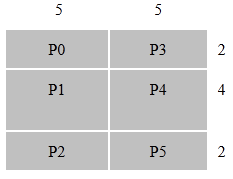
\includegraphics{CrGhostIr}
\centering
\caption{Creating an Array with Ghost Cells}
\label{crghostir}
\end{figure}

\end{desc}


\apih{CREATE_GHOSTS_IRREG_CONFIG}

\begin{capi}
int NGA_Create_ghost_irreg_config(int type, int ndim, int dims[], 
                                   width [], char *array_name, nblock[], 
                                   map[], int p_handle)
   array_name            - a unique character string                      \access{[input]} 
   type                  - data type (MT_DBL,MT_INT,MT_DCPL)              \access{[input]} 
   ndim                  - number of array dimensions                     \access{[input]} 
   dims[ndim]            - array of dimensions                            \access{[input]} 
   width[ndim]           - array of ghost cell widths                     \access{[input]} 
   nblock[ndim]          - no. of blocks each dimension is divided into   \access{[input]} 
   map[s]                - starting index for for each block; the size     
                           s is a sum of all elements of nblock array     \access{[input]} 
   p_handle              - processor list handle                          \access{[input]} 
\end{capi}

\begin{fapi}
logical function nga_create_ghosts_irreg_config(type, ndim, 
                                                dims, width, array_name, 
                                                map, nblock, 
                                                p_handle, g_a)
   character*(*) array_name       - a unique character string             \access{[input]} 
   integer       type             - data type (MT_DBL,MT_INT,MT_DCPL)     \access{[input]} 
   integer       ndim             - number of array dimensions            \access{[input]} 
   integer       dims(ndim)       - array of dimensions                   \access{[input]} 
   integer       width(ndim)      - array of ghost cell widths            \access{[input]} 
   integer       nblock(ndim)     - no. of blocks each dimension is
                                    divided into                          \access{[input]}
   integer       map(s)           - starting index for for each block; 
                                    the size s is a sum of all elements
                                    of nblock array                       \access{[input]} 
   integer       p_handle         - processor group handle                \access{[input]} 
   integer       g_a              - integer handle for future references  \access{[output]} 
\end{fapi}

\begin{cxxapi}
GlobalArray::GlobalArray(int type, int ndim, int dims[], int width[],
                         char *arrayname, int block[], int maps[],
                         PGroup* p_handle, char ghosts)
GlobalArray::GlobalArray(int type, int ndim, int64_t dims[], 
                         int64_t width[], char *arrayname, 
                         int64_t block[], int64_t maps[],
                         PGroup* p_handle,char ghosts)
   type          - data type (MT_DBL,MT_INT,MT_DCPL)                      \access{[input]}
   ndim          - number of array dimensions                             \access{[input]}
   dims[ndim]    - array of dimensions                                    \access{[input]}
   width[ndim]   - array of ghost cell widths                             \access{[input]}
   arrayname     - a unique character string                              \access{[input]}
   block[ndim]   - no. of blocks each dimension is divided into           \access{[input]}
   maps[s]       - starting index for for each block;
                   the size s is a sum of all elements of nblock array    \access{[input]}
   p_handle      - processor group handle                                 \access{[input]}
   ghosts        - this is a dummy parameter: added to increase the
                   number of arguments, inorder to avoid the conflicts
                   among constructors. (ghosts = 'g' or 'G')              \access{[input]}
\end{cxxapi}

\begin{desc}

Creates an array with ghost cells by following the user-specified distribution and returns integer handle representing the array.

This call is essentially the same as the NGA_Create_ghosts_irreg call, except for the processor list handle p_handle. It can be used to create mirrored arrays.

Return value: a non-zero array handle means the call was succesful.

This is a collective operation.

\end{desc}


\apih{CREATE_HANDLE}

\begin{capi}
int GA_Create_handle()
\end{capi}

\begin{fapi}
integer function ga_create_handle()
\end{fapi}

\begin{cxxapi}
GlobalArray::GlobalArray()
\end{cxxapi}

\begin{pyapi}
create_handle()
\end{pyapi}

\begin{desc}

  This function returns a Global Array handle that can then be used to
  create a new Global Array. This is part of a new API for creating
  Global Arrays that is designed to replace the old interface built
  around the NGA_Create_xxx calls. The sequence of operations is to
  begin with a call to GA_Greate_handle to get a new array handle. The
  attributes of the array, such as dimension, size, type, etc., can
  then be set using successive calls to the GA_Set_xxx subroutines.
  When all array attributes have been set, the GA_Allocate subroutine
  is called and the Global Array is actually created and memory for it
  is allocated.

  This is a collective operation.

\end{desc}


\apih{SET_ARRAY_NAME}

\begin{capi}
void GA_Set_array_name (int g_a, char *name)
   g_a                                                                    \access{[input]} 
   name                   - array name                                    \access{[input]} 
\end{capi}

\begin{fapi}
subroutine ga_set_array_name(g_a, name)
   integer         g_a            - global array handle                   \access{[input]} 
   character*(*)   name           - a unique character string             \access{[input]} 
\end{fapi}

\begin{cxxapi}
void GlobalArray::setArrayName(char *name) const
   name            - array name                                           \access{[input]}
\end{cxxapi}

\begin{pyapi}
set_array_name(int g_a, char *name)
\end{pyapi}

\begin{desc}

  This function can be used to assign a unique character string name
  to a Global Array handle that was obtained using the
  GA_Create_handle function.

  This is a collective operation.

\end{desc}


\apih{SET_DATA}

\begin{capi}
void GA_Set_data (int g_a, int ndim, int dims[], int type)
   g_a                                                                    \access{[input]} 
   ndim   - dimension of global array                                     \access{[input]} 
   dims[] - dimensions of global array                                    \access{[input]} 
   type   - data type of global array                                     \access{[input]} 
\end{capi}

\begin{fapi}
subroutine ga_set_data (g_a, ndim, dims, type)
   integer         g_a            - global array handle                   \access{[input]} 
   integer         ndim           - dimension of array                    \access{[input]} 
   integer         dims(ndim)     - array dimensions                      \access{[input]} 
   integer         type           - data type (MT_DBL,MT_INT,etc.)        \access{[input]} 
\end{fapi}

\begin{cxxapi}
void GlobalArray::setData(int ndim, int dims[], int type) const
void GlobalArray::setData(int ndim, int64_t dims[], int type) const
   ndim          - dimension of global array                             \access{[input]}
   dims          - dimensions of global array                            \access{[input]}
   type          - data type of global array                             \access{[input]}
\end{cxxapi}

\begin{pyapi}
set_data(int g_a, dims, int type)
\end{pyapi}

\begin{desc}

  This function can be used to set the array dimension, the coordinate
  dimensions, and the data type assigned to a Global Array handle
  obtained using the GA_Create_handle function.

  This is a collective operation.
\end{desc}


\apih{SET_IRREG_DISTR}

\begin{capi}
void GA_Set_irreg_distr(int g_a, int mapc[], int nblock[])
   g_a                                                                    \access{[input]} 
   mapc[s]       - starting index for each block; the size
                   s is the sum of all elements of the array
                   nblock                                                 \access{[input]} 
   nblock[ndim]  - number of blocks that each dimension is
                   divided into                                           \access{[input]} 
\end{capi}

\begin{fapi}
subroutine ga_set_irreg_distr(g_a, mapc, nblock)
    integer        g_a          - global array handle                     \access{[input]} 
    integer        map(s)       - starting index for for each
                                  block; the size s is a sum of
                                  all elements of nblock array            \access{[input]} 
    integer        nblock(ndim) - no. of blocks each dimension is
                                  divided into                            \access{[input]} 
\end{fapi}

\begin{cxxapi}
void GlobalArray::setIrregDistr(int mapc[], int nblock[]) const
void GlobalArray::setIrregDistr(int64_t mapc[], int64_t nblock[]) const
   mapc[s]           - starting index for each block; the size
                       s is the sum of all elements of the array nblock   \access{[input]}
   nblock[ndim]      - number of blocks that each dimension is
                       divided into                                       \access{[input]}
\end{cxxapi}

\begin{pyapi}
set_irreg_distr(int g_a, mapc, nblock)
\end{pyapi}

\begin{desc}

  This function can be used to partition the array data among the
  individual processors for a global array handle obtained using the
  GA_Create_handle function.

  The distribution is specified as a Cartesian product of
  distributions for each dimension. For example, the following figure
  demonstrates distribution of a 2-dimensional array 8x10 on 6 (or
  more) processors. nblock(2)=\{3,2\}, the size of mapc array is s=5 and
  array mapc contains the following elements mapc=\{1, 3, 7, 1, 6\}. The
  distribution is nonuniform because, P1 and P4 get 20 elements each
  and processors P0, P2, P3, and P5 only 10 elements each.

  The array width() is used to control the width of the ghost cell
  boundary around the visible data on each processor. The local data
  of the global array residing on each processor will have a layer
  width(n) ghosts cells wide on either side of the visible data along
  the dimension n.
An example is shown in Figure \ref{setirregdist}.

\begin{figure}
\centering
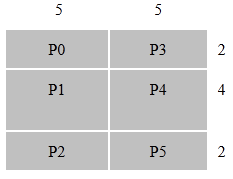
\includegraphics{SetIrregDist}
\caption{Set an Irregular Distribution}
\label{setirregdist}
\end{figure}

  This is a collective operation.

\end{desc}

\apih{SET_PGROUP}

\begin{capi}
void GA_Set_pgroup(int g_a, int p_handle)
   g_a                                                                    \access{[input]} 
   p_handle        processor group handle                                 \access{[input]} 
\end{capi}

\begin{fapi}
subroutine ga_set_pgroup(g_a, p_handle)
    integer        g_a          - global array handle                     \access{[input]} 
    integer        p_handle     - processor group handle                  \access{[input]} 
\end{fapi}

\begin{cxxapi}
void GlobalArray::setPGroup(PGroup *pHandle) const
   pHandle         - processor group handle                               \access{[input]}
\end{cxxapi}

\begin{pyapi}
set_pgroup(int g_a, int pgroup)
\end{pyapi}

\begin{desc}

  This function can be used to set the processor configuration
  assigned to a global array handle that was obtained using the
  GA_Create_handle function. It can be used to create mirrored arrays
  by using the mirrored array processor configuration in this function
  call. It can also be used to create an array on a processor group by
  using a processor group handle in this call.

  This is a collective operation.

\end{desc}

\apih{SET_RESTRICTED}

\begin{capi}
void GA_Set_restricted(int g_a, int list[], int nproc)
   g_a           - global array handle                                    \access{[input]} 
   list[nproc]   - list of processor IDs that
                   contain data                                           \access{[input]} 
   nproc         - number of processors that contain
                   data                                                   \access{[input]} 
\end{capi}

\begin{fapi}
subroutine ga_set_restricted(g_a, list, nproc)
    integer        g_a          - global array handle                     \access{[input]} 
    integer        list(nproc)  - list of processor IDs that
                                  contain data                            \access{[input]} 
    integer        nproc        - number of processors that
                                  contain data                            \access{[input]} 
\end{fapi}

\begin{cxxapi}
void GlobalArray::setRestricted(int list[], int nprocs) const
   list               - list of processors that should contain data       \access{[input]}
   nprocs             - number of processors in list                      \access{[input]}
\end{cxxapi}

\begin{desc}

  This function restricts data in the global array g_a to only the
  nproc processors listed in the array list. The value of nproc must be
  less than or equal to the number of available processors. If this
  call is used in conjunction with GA_Set_irreg_distr, then the
  decomposition in the GA_Set_irreg_distr call must be done assuming
  that the number of processors is nproc. The data that ordinarily
  would be mapped to process 0 is mapped to the process in list[0],
  the data that would be mapped to process 1 will be mapped to
  list[1], etc. This can be used to remap the data distribution to
  different processors, even if nproc equals the number of available
  processors.

This is a collective operation.

\end{desc}

\apih{SET_RESTRICTED_RANGE}

\begin{capi}
void GA_set_restricted_range(int g_a, int lo_proc, int hi_proc)
   g_a                          - global array handle                     \access{[input]} 
   lo_proc, hi_proc             - range of processors (inclusive)
                                  that contain data                       \access{[input]} 
\end{capi}

\begin{fapi}
subroutine ga_set_restricted_range(g_a, lo_proc, hi_proc)
    integer        g_a               - global array handle                \access{[input]} 
    integer        lo_proc, hi_proc  - range of processors
                                       (inclusive) that contain
                                        data                              \access{[input]} 
\end{fapi}

\begin{cxxapi}
void GlobalArray::setRestrictedRange(int lo_proc, int hi_proc) const
   lo_proc               - low end of processor range                    \access{[input]}
   hi_proc               - high end of processor range                   \access{[input]}
\end{cxxapi}

\begin{desc}

  This function restricts data in the global array to the range of
  processors beginning with lo_proc and ending with hi_proc. Both
  lo_proc and hi_proc must be less than or equal to the total number
  of processors minus one (e.g., in the range [0,N-1], where N is the
  total number of processors) and lo_proc must be less than or equal
  to hi_proc. If lo_proc = 0 and hi_proc = N-1 then this call has no
  effect on the data distribution.

  This is a collective operation.

\end{desc}

\apih{SET_GHOSTS}

\begin{capi}
void GA_Set_ghosts(int g_a, int width[])
   g_a                                                                    \access{[input]} 
   width[ndim]    - array of ghost cell widths                            \access{[input]} 
\end{capi}

\begin{fapi}
subroutine ga_set_ghosts(g_a, width)
    integer        g_a               - global array handle                \access{[input]} 
    integer        width(ndim)       - array of ghost cell widths         \access{[input]} 
\end{fapi}

\begin{cxxapi}
void GlobalArray::setGhosts(int width[]) const
void GlobalArray::setGhosts(int64_t width[]) const
   width[ndim]             - array of ghost cell widths                  \access{[input]}
\end{cxxapi}

\begin{pyapi}
set_ghosts(int g_a, width)
\end{pyapi}

\begin{desc}

  This function can be used to set the ghost cell widths for a global
  array handle that was obtained using the GA_Create_handle function.
  The ghosts cells widths indicate how many ghost cells are used to
  pad the locally held array data along each dimension. The padding
  can be set independently for each coordinate dimension.

  This is a collective operation.

\end{desc}

\apih{SET_CHUNK}

\begin{capi}
void GA_Set_chunk(int g_a, int chunk[])
   g_a                                                                    \access{[input]} 
   chunk[]        - array of chunk widths                                 \access{[input]} 
\end{capi}

\begin{fapi}
subroutine ga_set_chunk(g_a, chunk)
   integer         g_a               - global array handle                \access{[input]} 
   integer         chunk(ndim)       - array of chunk widths              \access{[input]} 
\end{fapi}

\begin{cxxapi}
void GlobalArray::setChunk(int chunk[]) const
void GlobalArray::setChunk(int64_t chunk[]) const
   chunk           - array of chunk widths                               \access{[input]}
\end{cxxapi}

\begin{pyapi}
set_chunk(int g_a, chunk)
\end{pyapi}

\begin{desc}

  This function is used to set the chunk array for a global array
  handle that was obtained using the GA_Create_handle function. The
  chunk array is used to determine the minimum number of array
  elements assigned to each processor along each coordinate direction.

  This is a collective operation.

\end{desc}

\apih{SET_BLOCK_CYCLIC}

\begin{capi}
void GA_Set_block_cyclic(int g_a, int dims[])
   g_a            - global array handle                                   \access{[input]} 
   dims[]         - array of block dimensions                             \access{[input]} 
\end{capi}

\begin{fapi}
subroutine ga_set_block_cyclic(g_a, dims)
   integer          g_a              - global array handle                \access{[input]} 
   integer          dims(ndim)       - array of block dimensions          \access{[input]} 
\end{fapi}

\begin{cxxapi}
void GlobalArray::setBlockCyclic(int dims[]) const
   dims             - array of block dimensions                          \access{[input]}
\end{cxxapi}

\begin{pyapi}
set_block_cyclic(int g_a, dims)
\end{pyapi}

\begin{desc}

  This subroutine is used to create a global array with a simple
  block-cyclic data distribution. The array is broken up into blocks
  of size dims and each block is numbered sequentially using a column
  major indexing scheme. The blocks are then assigned in a simple
  round-robin fashion to processors. 

Figure \ref{stblkcy} illustrates an array containing 25 blocks distributed on 4 processors.

  Blocks at the edge of the array may be smaller than the block size
  specified in dims. In the example below, blocks
  4, 9, 14, 19, 20, 21, 22, 23, and 24 might be smaller than the remaining
  blocks. Most global array operations are insensitive to whether or
  not a block-cyclic data distribution is used, although performance
  may be slower in some cases if the global array is using a
  block-cyclic data distribution. Individual data blocks can be
  accessesed using the block-cyclic access functions.

\begin{figure}
\centering
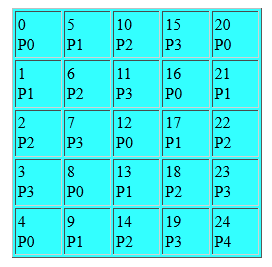
\includegraphics{StBlkCy}
\caption{Set Block Cyclic Data Distribution}
\label{stblkcy}
\end{figure}

  This is a collective operation.

\end{desc}

\apih{SET_BLOCK_CYCLIC_PROC_GRID}

\begin{capi}
void GA_Set_block_cyclic(int g_a, int dims[], int proc_grid[])
   g_a            - global array handle                                   \access{[input]} 
   dims[]         - array of block dimensions                             \access{[input]} 
   proc_grid[]    - processor grid dimensions                             \access{[input]} 
\end{capi}

\begin{fapi}
subroutine ga_set_block_cyclic_proc_grid(g_a, dims, proc_grid)
   integer          g_a              - global array handle                \access{[input]} 
   integer          dims(ndim)       - array of block dimensions          \access{[input]} 
\end{fapi}

\begin{cxxapi}
void GlobalArray::setBlockCyclicProcGrid(int dims[], int proc_grid[]) const
  dims             - array of block dimensions                            \access{[input]}
  proc_grid        - processor grid dimensions                            \access{[input]}
\end{cxxapi}

\begin{pyapi}
set_block_cyclic_proc_grid(int g_a, block, proc_grid)
\end{pyapi}

\begin{desc}

  This subroutine is used to create a global array with a
  SCALAPACK-type block cyclic data distribution. The user specifies
  the dimensions of the processor grid in the array proc_grid. The
  product of the processor grid dimensions must equal the number of
  total number of processors and the number of dimensions in the
  processor grid must be the same as the number of dimensions in the
  global array. The data blocks are mapped onto the processor grid in
  a cyclic manner along each of the processor grid axes. 

Figure \ref{setblkcyprocgrid} illustrates an array consisting of 25 data blocks distributed on 6 processors.

The 6 processors are configured in a 3 by 2 processor grid. Blocks at the edge of the array may be smaller than the block size specified in dims. Most global array operations  are insensitive to whether or not a block-cyclic data distribution is used, although performance may be slower in some cases if the global array is using a block-cyclic data distribution. Individual data blocks can be accessesed using the block-cyclic access functions.

\begin{figure}
\centering
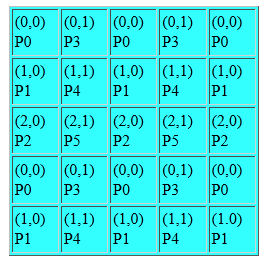
\includegraphics{SetBlkCyProcGrid}
\caption{Creating a SCALAPACK-type Block Cyclic Data Distribution}
\label{setblkcyprocgrid}
\end{figure}

  This is a collective operation.

\end{desc}

\apih{ALLOCATE}

\begin{capi}
int GA_Allocate(int g_a)
   ga                                                                     \access{[input]} 
\end{capi}

\begin{fapi}
logical function ga_allocate(g_a)
    integer         g_a              - global array handle                \access{[input]} 
\end{fapi}

\begin{cxxapi}
int GlobalArray::allocate() const
\end{cxxapi}

\begin{pyapi}
allocate(int g_a)
   g_a (int) - the array handle
\end{pyapi}

\begin{desc}

  This function allocates the memory for the global array handle
  originally obtained using the GA_Create_handle function. At a
  minimum, the GA_Set_data function must be called before the memory
  is allocated. Other GA_Set_xxx functions can also be called before
  invoking this function.

Returns True if allocation of g_a was successful.

  This is a collective operation.

\end{desc}

\apih{UPDATE_GHOSTS}

\begin{capi}
void GA_Update_ghosts(int g_a)
\end{capi}

\begin{fapi}
subroutine ga_update_ghosts(g_a)
   integer          g_a                                                   \access{[input]} 
\end{fapi}

\begin{cxxapi}
void GlobalArray::updateGhosts() const
\end{cxxapi}

\begin{pyapi}
update_ghosts(int g_a)
\end{pyapi}

\begin{desc}

  This call updates the ghost cell regions on each processor with the
  corresponding neighbor data from other processors. The operation
  assumes that all data is wrapped around using periodic boundary data
  so that ghost cell data that goes beyound an array boundary is
  wrapped around to the other end of the array. The GA_Update_ghosts
  call contains two GA_Sync calls before and after the actual update
  operation. For some applications these calls may be unecessary, if
  so they can be removed using the GA_Mask_sync subroutine. 
This is a collective operation.

\end{desc}

\apih{UPDATE_GHOST_DIR}

\begin{capi}
int NGA_Update_ghost_dir(int g_a, int dimension, int idir, int cflag)
   g_a                                                                    \access{[input]} 
   dimension      - array dimension that is to be updated                 \access{[input]} 
   idir           - direction of update (+/- 1)                           \access{[input]} 
   cflag          - flag (0/1) to include corners in update               \access{[input]} 
\end{capi}

\begin{fapi}
logical function nga_update_ghost_dir(g_a,dimension,idir,cflag)
   integer          g_a                                                   \access{[input]} 
   integer          dimension    - array dimension that is to be
                                   updated                                \access{[input]} 
   integer          idir         - direction of update (+/-1)             \access{[input]} 
   logical          cflag        - flag to include corners in update      \access{[input]} 
\end{fapi}

\begin{cxxapi}
int GlobalArray::updateGhostDir(int dimension, int idir, int cflag) const
   dimension        - array dimension that is to be updated               \access{[input]}
   idir             - direction of update (+/- 1)                         \access{[input]}
   cflag            - flag (0/1) to include corners in update             \access{[input]}
\end{cxxapi}

\begin{pyapi}
update_ghost_dir(int g_a, int dimension, int dir, int flag)
\end{pyapi}

\begin{desc}

  This function can be used to update the ghost cells along individual
  directions. It is designed for algorithms that can overlap updates
  with computation. The variable dimension indicates which coordinate
  direction is to be updated (e.g. dimension = 1 would correspond to
  the y axis in a two or three dimensional system), the variable idir
  can take the values +/-1 and indicates whether the side that is to
  be updated lies in the positive or negative direction, and cflag
  indicates whether or not the corners on the side being updated are
  to be included in the update. The following calls would be
  equivalent to a call to GA_Update_ghosts for a 2-dimensional system:

\begin{codeseg}
     status = NGA_Update_ghost_dir(g_a,0,-1,1);
     status = NGA_Update_ghost_dir(g_a,0,1,1);
     status = NGA_Update_ghost_dir(g_a,1,-1,0);
     status = NGA_Update_ghost_dir(g_a,1,1,0);
\end{codeseg}

         The variable cflag is set equal to 1 (or non-zero) in the
         first two calls so that the corner ghost cells are update, it
         is set equal to 0 in the second two calls to avoid redundant
         updates of the corners. Note that updating the ghosts cells
         using several independent calls to the nga_update_ghost_dir
         functions is generally not as efficient as using
         GA_Update_ghosts unless the individual calls can be
         effectively overlapped with computation.

This is a  collective operation.

\end{desc}

\apih{HAS_GHOSTS}

\begin{capi}
int GA_Has_ghosts(int g_a)
\end{capi}

\begin{fapi}
logical function ga_has_ghosts(g_a)
   integer          g_a                                                   \access{[input]} 
\end{fapi}

\begin{cxxapi}
int GlobalArray::hasGhosts() const
\end{cxxapi}

\begin{pyapi}
has_ghosts(int g_a)
\end{pyapi}

\begin{desc}

This function returns 1 if the global array has some dimensions for which the ghost cell width is greater than zero, it returns 0 otherwise.
This is a collective operation.

\end{desc}

\apih{ACCESS_GHOSTS}

\begin{capi}
void NGA_Access_ghosts(int g_a, int dims[], void *ptr, int ld[])
   g_a                                                                    \access{[input]} 
   dims[ndim]     - array of dimensions of local patch, including
                    ghost cells                                           \access{[output]} 
   ptr            - returns an index corresponding to the origin
                    the global array patch held locally on the
                    processor                                             \access{[output]} 
   ld[ndim-1]     - physical dimenstions of the local array patch,
                    including ghost cells                                 \access{[output]} 
\end{capi}

\begin{fapi}
subroutine nga_access_ghosts(g_a, dims, index, ld)
   integer          g_a                                                   \access{[input]} 
   integer          dims(ndim)  - array of dimensions of local
                                  patch, including ghost
                                  cells                                   \access{[output]} 
   integer          index       - returns an index corresponding
                                  to the origin the global array
                                  patch held locally on the
                                  processor                               \access{[output]} 
   integer          ld(ndim)    - physical dimenstions of the
                                  local array patch, including
                                  ghost cells                             \access{[output]} 
\end{fapi}

\begin{cxxapi}
void GlobalArray::accessGhosts(int dims[], void *ptr, int ld[]) const
void GlobalArray::accessGhosts(int64_t dims[], void *ptr, int64_t ld[]) const
   dims[ndim]           - array of dimensions of local patch,
                          including ghost cells                           \access{[output]}
   ptr                  - returns an index corresponding to the origin
                          the global array patch held locally on
                          the processor                                   \access{[output]}
   ld[ndim-1]           - physical dimensions of the local array patch,
                          including ghost cells                           \access{[output]}
\end{cxxapi}

\begin{pyapi}
access_ghosts(int g_a)
   g_a (int) - the array handle
\end{pyapi}

\begin{desc}

  Provides access to the local patch of the global array. Returns
  leading dimension ld and and pointer for the data.  This routine
  will provide access to the ghost cell data residing on each
  processor. Calls to NGA_Access_ghosts should normally follow a call
  to NGA_Distribution that returns coordinates of the visible data
  patch associated with a processor. You need to make sure that the
  coordinates of the patch are valid (test values returned from
  NGA_Distribution).

You can only access local data.
This is a local operation.

\end{desc}

\apih{ACCESS_GHOST_ELEMENT}

\begin{capi}
void NGA_Access_ghost_element(int g_a, void *ptr, int subscript[],
                              int ld[])
   g_a                                                                    \access{[input]} 
   index            - index pointing to location of element
                      indexed by subscript[]                              \access{[output]} 
   subscript[ndim]  - array of integers that index desired
                      element                                             \access{[input]} 
   ld[ndim-1]       - array of strides for local data patch.
                      These include ghost cell widths.                    \access{[output]} 
\end{capi}

\begin{fapi}
subroutine nga_access_ghost_element(g_a, index, subscript, ld)
   integer          g_a                                                   \access{[input]} 
   integer          index           - index pointing to location 
                                      of element
                                      indexed by subscript()              \access{[output]} 
   integer          subscript(ndim) - array of integers that 
                                      index desired element               \access{[input]} 
   integer          ld(ndim-1)      - array of strides for local 
                                      data patch. These include 
                                      ghost cell widths.                  \access{[output]} 
\end{fapi}

\begin{cxxapi}
void GlobalArray::accessGhostElement(void *ptr, int subscript[], int ld[]) const
void GlobalArray::accessGhostElement(void *ptr, int64_t subscript[], int64_t ld[]) const
   ptr              - index pointing to location of element
                      indexed by subscript[]                              \access{[output]}
   subscript[ndim]  - array of integers that index desired element        \access{[input]}
   ld[ndim-1]       - array of strides for local data patch.
                      These include ghost cell widths.                    \access{[output]}
\end{cxxapi}

\begin{pyapi}
access_ghost_element(int g_a, subscript, ld)
   g_a (int)                             - the array handle
   subscript (1D array-like of integers) - index of the desired element
\end{pyapi}

\begin{desc}

  This function can be used to return a pointer to any data element in
  the locally held portion of the global array and can be used to
  directly access ghost cell data. The array subscript refers to the
  local index of the element relative to the origin of the local patch
  (which is assumed to be indexed by (0,0,...)). 

  This is a local operation.

\end{desc}

\apih{TOTAL_BLOCKS}

\begin{capi}
int GA_Total_blocks(int g_a)
   g_a                                                                    \access{[input]} 
\end{capi}

\begin{fapi}
integer function ga_total_blocks(g_a)
   integer g_a                                                            \access{[input]} 
\end{fapi}

\begin{cxxapi}
int GlobalArray::totalBlocks() const
\end{cxxapi}

\begin{pyapi}
total_blocks(int g_a)
\end{pyapi}

\begin{desc}

This function returns the total number of blocks contained in a global array with a block-cyclic data distribution. This is a local operation.

\end{desc}

\apih{GET_BLOCK_INFO}

\begin{capi}
void GA_Get_block_info(int g_a, int num_blocks[], int block_dims[])
   g_a                                                                    \access{[input]} 
   num_blocks[ndim]   - number of blocks along each axis                  \access{[output]} 
   block_dims[ndim]   - dimensions of block                               \access{[output]} 
\end{capi}

\begin{fapi}
subroutine ga_get_block_info(g_a, num_blocks, block_dims)
   integer       g_a                                                      \access{[input]} 
   integer       num_blocks(ndim)   - number of blocks along each axis    \access{[output]} 
   integer       block_dims(ndim)   - dimensions of block                 \access{[output]} 
\end{fapi}

\begin{cxxapi}
void GlobalArray::getBlockInfo(int num_blocks[], int block_dims[])
num_blocks[ndim]        - array containing number of blocks along each
                          coordinate direction                            \access{[output]}
block_dims[ndim]        - array containing block dimensions               \access{[output]}
\end{cxxapi}

\begin{pyapi}
get_block_info(int g_a)
   g_a (int) - the array handle
\end{pyapi}

\begin{desc}

This subroutine returns information about the block-cyclic distribution associated with global array g_a. The number of blocks along each of the array axes are returned in the array num_blocks and the dimensions of the individual blocks, specified in the GA_Set_block_cyclic or GA_Set_block_cyclic_proc_grid subroutines, are returned in block_dims. This is a local function.

\end{desc}

\apih{DUPLICATE}

\begin{capi}
int GA_Duplicate(int g_a, char* array_name)
   array_name    - a character string                                     \access{[input]} 
   g_a           - integer handle for reference array                     \access{[input]} 
\end{capi}

\begin{fapi}
logical function ga_duplicate(g_a, g_b, array_name)
   character*(*) array_name    - a character string                       \access{[input]} 
   integer g_a                 - Integer handle for reference array       \access{[input]} 
   integer g_b                 - Integer handle for new array             \access{[output]} 
\end{fapi}

\begin{cxxapi}
GlobalArray::GlobalArray(const GlobalArray &g_a, char *arrayname)
GlobalArray::GlobalArray(const GlobalArray &g_a)
GlobalArray * GAServices::createGA(const GlobalArray *g_b, char *arrayname)
GlobalArray * GAServices::createGA(const GlobalArray &g_b)
   g_b                          - integer handle for reference array      \access{[input]}
   arrayname                    - a character string                      \access{[input]}
\end{cxxapi}

\begin{pyapi}
duplicate(int g_a, char *name='')
   g_a (int)     - the array handle
   name (string) - the new name of the created array
\end{pyapi}

\begin{desc}

Creates a new array by applying all the properties of another existing array. It returns an array handle.

Return value: a non-zero array handle means the call was succesful.
This is a collective operation.

\end{desc}

\apih{DESTROY}

\begin{capi}
void GA_Destroy(int g_a)
   g_a   - array handle                                                   \access{[input]} 
\end{capi}

\begin{fapi}
logical function ga_destroy(g_a)  
   integer g_a                                                            \access{[input]} 
\end{fapi}

\begin{cxxapi}
GlobalArray::~GlobalArray()
void GlobalArray::destroy()
\end{cxxapi}

\begin{pyapi}
destroy(int g_a)
\end{pyapi}

\begin{desc}

Deallocates the array and frees any associated resources.

This is a collective operation.

\end{desc}

\apih{TERMINATE}

\begin{capi}
void GA_Terminate()
\end{capi}

\begin{fapi}
subroutine ga_terminate()
\end{fapi}

\begin{cxxapi}
void GA::Terminate()
\end{cxxapi}

\begin{pyapi}
terminate()
\end{pyapi}

\begin{desc}

Delete all active arrays and destroy internal data structures.

This is a collective operation.

\end{desc}

\apih{SYNC}

\begin{capi}
void GA_Sync()
\end{capi}

\begin{fapi}
subroutine ga_sync()
\end{fapi}

\begin{cxxapi}
GAServices::sync()
GA::sync()
\end{cxxapi}

\begin{pyapi}
sync()
\end{pyapi}

\begin{desc}

Synchronize processes (a barrier) and ensure that all GA operations completed.

This is a collective operation.

\end{desc}

\apih{MASK_SYNC}

\begin{capi}
void GA_Mask_sync(int first,int last)
   first           - mask (0/1) for prior internal synchronization        \access{[input]} 
   last            - mask (0/1) for post internal synchronization         \access{[input]} 
\end{capi}

\begin{fapi}
subroutine ga_mask_sync(first,last)
   logical first   - mask for prior internal synchronization              \access{[input]} 
   logical last    - mask for post internal synchronization               \access{[input]} 
\end{fapi}

\begin{cxxapi}
void GAServices::maskSync(int first, int last)
void GA::maskSync(int first, int last)
   first          - masks the sync at the begining of the collective call \access{[input]}
   last           - masks the sync at the end of the collective call      \access{[input]}
\end{cxxapi}

\begin{pyapi}
mask_sync(int first, int last)
   first (bool) - mask for prior internal synchronization
   last (bool) - mask for post internal synchronization
\end{pyapi}

\begin{desc}

This subroutine can be used to remove synchronization calls from around collective operations. Setting the parameter first = .false. removes the synchronization prior to the collective operation, setting last = .false. removes the synchronization call after the collective operation. This call is applicable to all collective operations. It most be invoked before each collective operation.
This is a  collective operation.

\end{desc}

\apih{ZERO}

\begin{capi}
void GA_Zero(int g_a)
   g_a - array handle                                                     \access{[input]} 
\end{capi}

\begin{fapi}
subroutine ga_zero(g_a)
   integer g_a                                                            \access{[input]} 
\end{fapi}

\begin{cxxapi}
void GlobalArray::zero() const
\end{cxxapi}

\begin{pyapi}
zero(int g_a, lo=None, hi=None)
\end{pyapi}

\begin{desc}

Sets value of all elements in the array to zero.

This is a collective operation.

\end{desc}

\apih{FILL}

\begin{capi}
void GA_Fill(int g_a, void *value)
   g_a     - array handle                                                 \access{[input]} 
   value   - pointer to the value of appropriate type 
             (double/DoubleComplex/long)
             that matches array type                                      \access{[input]} 
\end{capi}

\begin{fapi}
subroutine ga_fill(g_a, s)
   integer g_a                                                            \access{[input]} 
   double precision/complex/integer s                                     \access{[input]} 
\end{fapi}

\begin{cxxapi}
void GlobalArray::fill(void *value) const
   value        - pointer to the value of appropriate type
                  (double/DoubleComplex/long) that matches array type.    \access{[input]}
\end{cxxapi}

\begin{pyapi}
fill(int g_a, value, lo=None, hi=None)
   g_a (int)                      - the array handle
   lo (1D array-like of integers) - lower bound patch coordinates, inclusive
   hi (1D array-like of integers) - higher bound patch coordinates, exclusive
\end{pyapi}

\begin{desc}

Assign a single value to all elements in the array.

This is a collective operation.

\end{desc}

\apih{DOT}

\begin{capi}
int GA_Idot(int g_a, int g_b) 
long GA_Ldot(int g_a, int g_b) 
float GA_Fdot(int g_a, int g_b) 
double GA_Ddot(int g_a, int g_b) 
DoubleComplex GA_Zdot(int g_a, int g_b) 
   g_a, g_b   - array handles                                             \access{[input]} 
\end{capi}

\begin{fapi}
double precision function ga_ddot(g_a, g_b)
double complex function ga_zdot(g_a, g_b)
   integer g_a, g_b                                                       \access{[input]} 
\end{fapi}

\begin{cxxapi}
int GlobalArray::idot(const GlobalArray * g_a) const
long GlobalArray::ldot(const GlobalArray * g_a) const
float GlobalArray::fdot(const GlobalArray * g_a) const
double GlobalArray::ddot(const GlobalArray * g_a) const
DoubleComplex GlobalArray::zdot(const GlobalArray * g_a) const
g_a - GlobalArray                                                         \access{[input]}
\end{cxxapi}

\begin{pyapi}
dot(int g_a, int g_b, alo=None, ahi=None, blo=None, bhi=None, int ta=False, 
int tb=False)
   g_a (int)                       - the array handle
   g_b (int)                       - the array handle
   alo (1D array-like of integers) - lower bound patch coordinates of g_a, 
                                     inclusive
   ahi (1D array-like of integers) - higher bound patch coordinates of g_a, 
                                     exclusive
   blo (1D array-like of integers) - lower bound patch coordinates of g_b, 
                                     inclusive
   bhi (1D array-like of integers) - higher bound patch coordinates of g_b, 
                                     exclusive
   ta (bool)                       - whether the transpose operator should 
                                     be applied to g_a True=applied
   tb (bool)                       - whether the transpose operator should 
                                     be applied to g_b True=applied
\end{pyapi}

\begin{desc}

Computes the element-wise dot product of the two arrays which must be of the same types and same number of elements.
      Return value = SUM_ij a(i,j)*b(i,j)


This is a collective operation.

\end{desc}

\apih{SCALE}

\begin{capi}
void GA_Scale(int g_a, void *value)
   g_a     - array handle                                                 \access{[input]} 
   value   - pointer to the value of appropriate type 
             (double/DoubleComplex/long)
             that matches array type                                      \access{[input]} 
\end{capi}

\begin{fapi}
subroutine ga_scale(g_a, s) 
   integer g_a                                                            \access{[input]} 
   double precision/complex/integer s                                     \access{[input]} 
\end{fapi}

\begin{cxxapi}
void GlobalArray::scale(void *value) const
   value            - pointer to the value of appropriate type            \access{[input]}
\end{cxxapi}

\begin{pyapi}
scale(int g_a, value, lo=None, hi=None)
\end{pyapi}

\begin{desc}

Scales an array by the constant s. Note that the library is unable to detect errors when the pointed value is of a different type than the array.

This is a collective operation.

\end{desc}

\apih{ADD}

\begin{capi}
void GA_Add(void *alpha, int g_a, void* beta, int g_b, int g_c)
   g_a, g_b, g_c                        - array handles                   \access{[input]} 
   double/complex/int      *alpha       - scale factor                    \access{[input]} 
   double/complex/int      *beta        - scale factor                    \access{[input]} 
\end{capi}

\begin{fapi}
subroutine ga_add(alpha, g_a, beta, g_b, g_c)
   integer g_a, g_b, g_c                                                  \access{[input]} 
   double precision/complex/integer alpha, beta                           \access{[input]} 
\end{fapi}

\begin{cxxapi}
void GlobalArray::add(void *alpha, const GlobalArray * g_a, void *beta,
                      const GlobalArray * g_b) const
   alpha                - scale factor                                    \access{[input]}
   g_a                  - array                                           \access{[input]}
   beta                 - scale factor                                    \access{[input]}
   g_b                  - array                                           \access{[input]}
\end{cxxapi}

\begin{pyapi}
add(int g_a, int g_b, int g_c, alpha=None, beta=None, alo=None, ahi=None, blo=None, bhi=None, clo=None, chi=None)
   g_a (int)                       - the array handle
   g_b (int)                       - the array handle
   g_c (int)                       - the array handle
   alpha (object)                  - multiplier (converted to appropriate type)
   beta (object)                   - multiplier (converted to appropriate type)
   alo (1D array-like of integers) - lower bound patch coordinates of 
                                     g_a, inclusive
   ahi (1D array-like of integers) - higher bound patch coordinates of 
                                     g_a, exclusive
   blo (1D array-like of integers) - lower bound patch coordinates of 
                                     g_b, inclusive
   bhi (1D array-like of integers) - higher bound patch coordinates of 
                                     g_b, exclusive
   clo (1D array-like of integers) - lower bound patch coordinates of 
                                     g_c, inclusive
   chi (1D array-like of integers) - higher bound patch coordinates of 
                                     g_c, exclusive
\end{pyapi}

\begin{desc}

The arrays (which must be the same shape and identically aligned) are added together element-wise.

\begin{codeseg}
        c = alpha * a  +  beta * b.
\end{codeseg}

The result (c) may replace one of the input arrays (a/b).

This is a collective operation.

\end{desc}

\apih{COPY}

\begin{capi}
void GA_Copy(int g_a, int g_b)
   g_a, g_b - array handles                                               \access{[input]} 
\end{capi}

\begin{fapi}
subroutine ga_copy(g_a, g_b) 
   integer g_a, g_b - array handles                                       \access{[input]} 
\end{fapi}

\begin{cxxapi}
void GlobalArray::copy(const GlobalArray *g_a) const
   g_a                 - GlobalArray to copy                              \access{[input]}
\end{cxxapi}

\begin{pyapi}
copy(int g_a, int g_b, alo=None, ahi=None, blo=None, bhi=None, int trans=False)
   g_a (int)                       - the array handle copying from
   g_b (int)                       - the array handle copying to
   alo (1D array-like of integers) - lower bound patch coordinates of 
                                     g_a, inclusive
   ahi (1D array-like of integers) - higher bound patch coordinates of 
                                     g_a, exclusive
   blo (1D array-like of integers) - lower bound patch coordinates of 
                                     g_b, inclusive
   bhi (1D array-like of integers) - higher bound patch coordinates of 
                                     g_b, exclusive
   trans (bool) - whether the transpose operator should be applied True=applied
\end{pyapi}

\begin{desc}

Copies elements in array represented by g_a into the array represented by g_b. The arrays must be the same type, shape, and identically aligned.

This is a collective operation.

\end{desc}

\apih{SET_MEMORY_LIMIT}

\begin{capi}
void GA_Set_memory_limit(size_t limit)
   limit    - the amount of memory in bytes per process                   \access{[input]} 
\end{capi}
\begin{fapi}
subroutine ga_set_memory_limit(limit)
   integer limit  - the amount of memory in bytes per process             \access{[input]} 
\end{fapi}

\begin{cxxapi}
void GlobalArray::setMemoryLimit(size_t limit);
   limit                   - the amount of memory in bytes per process    \access{[input]}
\end{cxxapi}

\begin{desc}

Sets the amount of memory to be used (in bytes) per process

This is a local operation.

\end{desc}

\apih{GET}

\begin{capi}
void NGA_Get(int g_a, int lo[], int hi[], void* buf, int ld[])
   g_a        - global array handle                                       \access{[input]} 
   ndim       - number of dimensions of the global array                  \access{[input]} 
   lo[ndim]   - array of starting indices for global array section        \access{[input]}  
   hi[ndim]   - array of ending indices for global array section          \access{[input]}  
   buf        - pointer to the local buffer array where the data goes     \access{[output]} 
   ld[ndim-1] - array specifying leading dimensions/strides/extents 
                for buffer array                                          \access{[input]} 
\end{capi}

\begin{f2dapi}
subroutine ga_get(g_a, ilo, ihi, jlo, jhi, buf, ld)
   integer g_a                                                            \access{[input]} 
   integer ilo, ihi, jlo, jhi                                             \access{[input]} 
   double precision/complex/integer buf                                   \access{[output]} 
   integer ld                                                             \access{[input]} 
\end{f2dapi}

\begin{fapi}
subroutine nga_get(g_a, lo, hi,  buf, ld)
   integer g_a        - global array handle                               \access{[input]} 
   integer ndim       - number of dimensions of the global array          \access{[input]} 
   integer lo(ndim)   - array of starting indices for global 
                        array section                                     \access{[input]} 
   integer hi(ndim)   - array of ending indices for global array 
                        section                                           \access{[input]} 
   <type> buf         - local buffer array where the data goes  to        \access{[output]} 
   integer ld(ndim-1) - array specifying leading dimensions for 
                        buffer array                                      \access{[input]} 
\end{fapi}

\begin{cxxapi}
void GlobalArray::get(int lo[], int hi[], void *buf, int ld[]) const
void GlobalArray::get(int64_t lo[], int64_t hi[], void *buf, int64_t ld[]) const
   lo[ndim]   - array of starting indices for global array section        \access{[input]}
   hi[ndim]   - array of ending indices for global array section          \access{[input]}
   buf        - pointer to the local buffer array where the data goes     \access{[output]}
   ld[ndim-1] -  array specifying leading dimensions/strides/extents
                 for buffer array                                         \access{[input]}
\end{cxxapi}

\begin{desc}

  Copies data from global array section to the local array buffer. The
  local array is assumed to be have the same number of dimensions as
  the global array. Any detected inconsistencies or errors in the input
  arguments are fatal.

Example: For the ga_get operation transfering data from the [10:14, 0:4]
section of 2-dimensional 15x10 global array into a local buffer 5x10
array we have: 

\begin{codeseg}
lo={10,0,} hi={14,4}, ld={10}  
\end{codeseg}

Figure \ref{get} shows the GET operation.

\begin{figure}
\centering
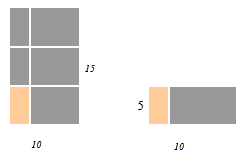
\includegraphics{GET}
\caption{Copying Data from 2-dimensional 15x10 Global Array into Local Buffer 5x10 Array}
\label{get}
\end{figure}

This is a one-sided operation.

 \end{desc}

\apih{PERIODIC_GET}

\begin{capi}
void NGA_Periodic_get(int g_a, int lo[], int hi[], void* buf, int ld[])
   g_a        - global array handle                                       \access{[input]} 
   ndim       - number of dimensions of the global array                  \access{[input]} 
   lo[ndim]   - array of starting indices for global array section        \access{[input]}  
   hi[ndim]   - array of ending indices for global array section          \access{[input]}  
   buf        - pointer to the local buffer array where the data goes     \access{[output]} 
   ld[ndim-1] - array specifying leading dimensions/strides/extents 
                for buffer array                                          \access{[input]} 
\end{capi}

\begin{fapi}
subroutine nga_periodic_get(g_a, lo, hi,  buf, ld)
   integer g_a        - global array handle                               \access{[input]} 
   integer ndim       - number of dimensions of the global array          \access{[input]} 
   integer lo(ndim)   - array of starting indices for global array 
                        section                                           \access{[input]} 
   integer hi(ndim)   - array of ending indices for global array 
                        section                                           \access{[input]} 
   <type> buf         - local buffer array where the data goes  to        \access{[output]} 
   integer ld(ndim-1) - array specifying leading dimensions for 
                        buffer array                                      \access{[input]} 
\end{fapi}

\begin{cxxapi}
void GlobalArray::periodicGet(int lo[], int hi[], void* buf, int ld[]) const
void GlobalArray::periodicGet(int64_t lo[], int64_t hi[], void* buf, int64_t ld[]) const
   lo[ndim]   - array of starting indices for global array section        \access{[input]}
   hi[ndim]   - array of ending indices for global array section          \access{[input]}
   buf        - pointer to the local buffer array where the data goes     \access{[output]}
   ld[ndim-1] - array specifying leading dimensions/strides/extents
                for buffer array                                          \access{[input]}
\end{cxxapi}

\begin{desc}

Same as nga_get except the indices can extend beyond the array boundary/dimensions in which case the library wraps them around.
This is a one-sided operation.

\end{desc}

\apih{STRIDED_GET}

\begin{capi}
void NGA_Strided_get(int g_a, int lo[], int hi[], int skip[], 
                     void* buf, int ld[])
   g_a        - global array handle                                       \access{[input]} 
   ndim       - number of dimensions of the global array                  \access{[input]} 
   lo[ndim]   - array of starting indices for global array section        \access{[input]}  
   hi[ndim]   - array of ending indices for global array section          \access{[input]} 
   skip[ndim] - array of strides for each dimension                       \access{[input]} 
   buf        - pointer to the local buffer array where the data goes     \access{[output]} 
   ld[ndim-1] - array specifying leading dimensions/strides/extents 
                for buffer array                                          \access{[input]} 
\end{capi}

\begin{fapi}
subroutine nga_strided_get(g_a, lo, hi, skip, buf, ld)
   integer g_a        - global array handle                               \access{[input]} 
   integer ndim       - number of dimensions of the global array          \access{[input]} 
   integer lo(ndim)   - array of starting indices for global 
                        array section                                     \access{[input]} 
   integer hi(ndim)   - array of ending indices for global array 
                        section                                           \access{[input]} 
   integer skip(ndim) - array of strides for each dimension               \access{[input]} 
   <type> buf         - local buffer array where the data comes from      \access{[output]} 
   integer ld(ndim-1) - array specifying leading dimensions for 
                        buffer array                                      \access{[input]} 
\end{fapi}

\begin{cxxapi}
void GlobalArray::stridedGet(int lo[], int hi[], int skip[],
                             void *buf, int ld[]) const
void GlobalArray::stridedGet(int64_t lo[], int64_t hi[], int64_t skip[],
                             void *buf, int64_t ld[]) const
   lo[ndim]   - array of starting indices for glob array section          \access{[input]}
   hi[ndim]   - array of ending indices for global array section          \access{[input]}
   skip[ndim] - array of strides for each dimension                       \access{[input]}
   buf        - pointer to local buffer array where data goes             \access{[output]}
   ld[ndim-1] - array specifying leading
   dimensions/strides/extents for buffer array                            \access{[input]}
\end{cxxapi}

\begin{desc}

This operation is the same as NGA_Get, except that the values corresponding to dimension n in buf correspond to every skip[n] values of the global array g_a. This is a one-sided operation.

\end{desc}

\apih{PUT}

\begin{capi}
void NGA_Put(int g_a, int lo[], int hi[], void* buf, int ld[])
   g_a        - global array handle                                       \access{[output]} 
   ndim       - number of dimensions of the global array                  \access{[input]} 
   lo[ndim]   - array of starting indices for global array section        \access{[input]}  
   hi[ndim]   - array of ending indices for global array section          \access{[input]}  
   buf        - pointer to the local buffer array where the data is       \access{[input]} 
   ld[ndim-1] - array specifying leading dimensions/strides/extents 
                for buffer array                                          \access{[input]} 
\end{capi}

\begin{f2dapi}
subroutine ga_put(g_a, ilo, ihi, jlo, jhi, buf, ld)
   integer g_a                                                            \access{[input]} 
   integer ilo, ihi, jlo, jhi                                             \access{[input]} 
   double precision/complex/integer buf                                   \access{[output]} 
   integer ld                                                             \access{[input]} 
\end{f2dapi}

\begin{fapi}
subroutine nga_put(g_a, lo, hi, buf, ld)
   integer g_a        - global array handle                               \access{[input]} 
   integer ndim       - number of dimensions of the global array          \access{[input]} 
   integer lo(ndim)   - array of starting indices for global array 
                        section                                           \access{[input]} 
   integer hi(ndim)   - array of ending indices for global array section  \access{[input]} 
   <type> buf         - local buffer array where the data comes from      \access{[output]} 
   integer ld(ndim-1) - array specifying leading dimensions for 
                        buffer array                                      \access{[input]} 
\end{fapi}

\begin{cxxapi}
void GlobalArray::put(int lo[], int hi[], void *buf, int ld[]) const
void GlobalArray::put(int64_t lo[], int64_t hi[], void *buf, 
                      int64_t ld[]) const
   lo[ndim]   - array of starting indices for global array section        \access{[input]}
   hi[ndim]   - array of ending indices for global array section          \access{[input]}
   buf        - pointer to the local buffer array where the data is       \access{[input]}
   ld[ndim-1] - array specifying leading dimensions/strides/extents
                for buffer array                                          \access{[input]}
\end{cxxapi}

\begin{pyapi}
put(int g_a, buffer, lo=None, hi=None)

Parameters:
        g_a (int) - the array handle
        buffer (array-like) - the data to put
        lo (1D array-like of integers) - lower bound patch coordinates, inclusive
        hi (array-like of integers) - higher bound patch coordinates, exclusive
\end{pyapi}

\begin{desc}

Copies data from the local array buffer to the global array section. The local array is assumed to have the same number of dimensions as the global array.
Any detected inconsistencies or errors in input arguments are fatal.

This is a one-sided operation.

\end{desc}

\apih{PERIODIC_PUT}

\begin{capi}
void NGA_Periodic_put(int g_a, int lo[], int hi[], void* buf, int ld[])
   g_a        - global array handle                                       \access{[output]} 
   ndim       - number of dimensions of the global array                  \access{[input]} 
   lo[ndim]   - array of starting indices for global array section        \access{[input]}  
   hi[ndim]   - array of ending indices for global array section          \access{[input]}  
   buf        - pointer to the local buffer array where the data is       \access{[input]} 
   ld[ndim-1] - array specifying leading dimensions/strides/extents 
                for buffer array                                          \access{[input]} 
\end{capi}

\begin{fapi}
subroutine nga_periodic_put(g_a, lo, hi,  buf, ld)
   integer g_a        - global array handle                               \access{[input]} 
   integer ndim       - number of dimensions of the global array          \access{[input]} 
   integer lo(ndim)   - array of starting indices for global 
                        array section                                     \access{[input]} 
   integer hi(ndim)   - array of ending indices for global array section  \access{[input]} 
   <type> buf         - local buffer array where the data comes from      \access{[output]} 
   integer ld(ndim-1) - array specifying leading dimensions for 
                        buffer array                                      \access{[input]} 
\end{fapi}

\begin{cxxapi}
void GlobalArray::periodicPut(int lo[], int hi[], void* buf, int ld[]) 
                              const
void GlobalArray::periodicPut(int64_t lo[], int64_t hi[], void* buf, 
                              int64_t ld[]) const
   lo[ndim]   - array of starting indices for global array section        \access{[input]}
   hi[ndim]   - array of ending indices for global array section          \access{[input]}
   buf        - pointer to the local buffer array where the data goes     \access{[input]}
   ld[ndim-1] - array specifying leading dimensions/strides/extents
                for buffer array                                          \access{[input]}
\end{cxxapi}

\begin{pyapi}
periodic_put(int g_a, buffer, lo=None, hi=None)
Parameters:
   g_a (int)                      - the array handle
   buffer (array-like)            - the data to put
   lo (1D array-like of integers) - lower bound patch coordinates, inclusive
   hi (array-like of integers)    - higher bound patch coordinates, exclusive

\end{pyapi}

\begin{desc}

Same as nga_put except the indices can extend beyond the array boundary/dimensions in which case the library wraps them around.
The indices can extend beyond the array boundary/dimensions in which case the libray wraps them around.
Copies data from local array buffer to the global array section.
The local array is assumed to be have the same number of dimensions as the global array. Any detected inconsitencies/errors in input arguments are fatal.
This is a one-sided operation.

\end{desc}

\apih{STRIDED_PUT}

\begin{capi}
void NGA_Strided_put(int g_a, int lo[], int hi[], int skip[], 
                     void* buf, int ld[])
   g_a        - global array handle                                       \access{[input]} 
   ndim       - number of dimensions of the global array                  \access{[input]} 
   lo[ndim]   - array of starting indices for global array section        \access{[input]}  
   hi[ndim]   - array of ending indices for global array section          \access{[input]} 
   skip[ndim] - array of strides for each dimension                       \access{[input]} 
   buf        - pointer to the local buffer array where the data goes     \access{[output]} 
   ld[ndim-1] - array specifying leading dimensions/strides/extents 
                for buffer array                                          \access{[input]} 
\end{capi}

\begin{fapi}
subroutine nga_strided_put(g_a, lo, hi, skip, buf, ld)
   integer g_a        - global array handle                               \access{[input]} 
   integer ndim       - number of dimensions of the global array          \access{[input]} 
   integer lo(ndim)   - array of starting indices for global 
                        array section                                     \access{[input]} 
   integer hi(ndim)   - array of ending indices for global array 
                        section                                           \access{[input]} 
   integer skip(ndim) - array of strides for each dimension               \access{[input]} 
   <type> buf         - local buffer array where the data comes from      \access{[output]} 
   integer ld(ndim-1) - array specifying leading dimensions for 
                        buffer array                                      \access{[input]} 
\end{fapi}

\begin{cxxapi}
void GlobalArray::stridedPut(int lo[], int hi[], int skip[],
                             void*buf, int ld[]) const
void GlobalArray::stridedPut(int64_t lo[], int64_t hi[], int64_t skip[],
                             void *buf, int64_t ld[]) const
   lo[ndim]   - array of starting indices for glob array section          \access{[input]}
   hi[ndim]   - array of ending indices for global array section          \access{[input]}
   skip[ndim] - array of strides for each dimension                       \access{[input]}
   buf        - pointer to local buffer array where data goes             \access{[input]}
   ld[ndim-1] - array specifying leading dimensions/strides/extents
                for buffer array                                          \access{[input]}
\end{cxxapi}

\begin{pyapi}
strided_put(int g_a, buffer, lo=None, hi=None, skip=None)
   g_a (int)                        - the array handle
   buffer (array-like)              - the data to put
   lo (1D array-like of integers)   - lower bound patch coordinates, inclusive
   hi (array-like of integers)      - higher bound patch coordinates, exclusive
   skip (1D array-like of integers) - strides for each dimension
\end{pyapi}

\begin{desc}

Strided version of put.  This operation is the same as NGA_Put, except that the values corresponding to dimension n in buf are copied to every skip[n] values of the global array g_a. 

Copies data from local array buffer to the global array section.

The local array is assumed to be have the same number of dimensions as the global array. 

Any detected inconsitencies/errors in input arguments are fatal.

This is a one-sided operation.

\end{desc}

\apih{ACC}

\begin{capi}
void NGA_Acc(int g_a, int lo[], int hi[], void* buf, int ld[], 
             void* alpha)
   g_a        - global array handle                                       \access{[input]} 
   ndim       - number of dimensions of the global array                  \access{[input]} 
   lo[ndim]   - array of starting indices for array section               \access{[input]}  
   hi[ndim]   - array of ending indices for array section                 \access{[input]} 
   buf        - pointer to the local buffer array                         \access{[input]} 
   ld[ndim-1] - array specifying leading dimensions/strides/extents 
                for buffer array                                          \access{[input]} 
   double/DoubleComplex/long *alpha scale factor                          \access{[input]} 
\end{capi}

\begin{f2dapi}
subroutine ga_acc(g_a, ilo, ihi, jlo, jhi, buf, ld, alpha)
   integer g_a                                                            \access{[input]} 
   integer ilo, ihi, jlo, jhi                                             \access{[input]} 
   double precision/complex buf                                           \access{[input]} 
   integer ld                                                             \access{[input]} 
   double precision/complex alpha                                         \access{[input]} 
\end{f2dapi}

\begin{fapi}
subroutine nga_acc(g_a, lo, hi, buf, ld, alpha)
   integer g_a        - global array handle                               \access{[input]} 
   integer ndim       - number of dimensions of the global array          \access{[input]} 
   integer lo(ndim)   - array of starting indices for global 
                        array section                                     \access{[input]} 
   integer hi(ndim)   - array of ending indices for global array section  \access{[input]} 
   <type> buf         - local buffer array where the local data is        \access{[output]} 
   integer ld(ndim-1) - array specifying leading dimensions for 
                        buffer array                                      \access{[input]} 
   <type> alpha       - scale argument for accumulate                     \access{[input]} 
\end{fapi}

\begin{cxxapi}
void GlobalArray::acc(int lo[], int hi[], void *buf,
                      int ld[], void *alpha) const
void GlobalArray::acc(int64_t lo[], int64_t hi[], void *buf,
                      int64_t ld[], void *alpha) const
   lo[ndim]   - array of starting indices for array section               \access{[input]}
   hi[ndim]   - array of ending indices for array section                 \access{[input]}
   buf        - pointer to the local buffer array                         \access{[input]}
   ld[ndim-1] - array specifying leading dimensions/strides/extents
                for buffer array                                          \access{[input]}
   alpha      - scale factor (double/DoubleComplex/long *)                \access{[input]}
\end{cxxapi}

\begin{pyapi}
acc(int g_a, buffer, lo=None, hi=None, alpha=None)
Parameters:
   g_a (int)           - the array handle
   buffer (array-like) - must be contiguous and have same number of 
                         elements as patch
   lo (1D array-like)  - lower bound patch coordinates, inclusive
   hi (1D array-like)  - higher bound patch coordinates, exclusive
   alpha (object)      - multiplier (converted to appropriate type)
\end{pyapi}

\begin{desc}

 Combines data from local array buffer with data in the global array section. The local array is assumed to be have the same number of dimensions as the global array.

If the buffer is not contiguous, a contiguous copy will be made.

    global array section (lo[],hi[]) += *alpha * buffer

This is a one-sided and atomic operation.

\end{desc}

\apih{PERIODIC_ACC}

\begin{capi}
void NGA_Periodic_acc(int g_a, int lo[], int hi[], void* buf, int ld[], 
                      void* alpha)
   g_a        - global array handle                                       \access{[input]} 
   ndim       - number of dimensions of the global array                  \access{[input]} 
   lo[ndim]   - array of starting indices for array section               \access{[input]}  
   hi[ndim]   - array of ending indices for array section                 \access{[input]} 
   buf        - pointer to the local buffer array                         \access{[input]} 
   ld[ndim-1] - array specifying leading dimensions/strides/extents 
                for buffer array                                          \access{[input]} 
                double/DoubleComplex/long *alpha     scale factor         \access{[input]} 
\end{capi}

\begin{fapi}
subroutine nga_periodic_acc(g_a, lo, hi, buf, ld, alpha)
   integer g_a        - global array handle                               \access{[input]} 
   integer ndim       - number of dimensions of the global array          \access{[input]} 
   integer lo(ndim)   - array of starting indices for global array 
                        section                                           \access{[input]} 
   integer hi(ndim)   - array of ending indices for global array 
                        section                                           \access{[input]} 
   <type> buf         - local buffer array where the local data is        \access{[output]} 
   integer ld(ndim-1) - array specifying leading dimensions for 
                        buffer array                                      \access{[input]} 
   <type> alpha       - scale argument for accumulate                     \access{[input]} 
\end{fapi}

\begin{cxxapi}
void GlobalArray::periodicAcc(int lo[], int hi[], void* buf,
                              int ld[], void* alpha) const
void GlobalArray::periodicAcc(int64_t lo[], int64_t hi[], void* buf,
                              int64_t ld[], void* alpha) const
   lo[ndim]   - array of starting indices for array section               \access{[input]}
   hi[ndim]   - array of ending indices for array section                 \access{[input]}
   buf        - pointer to the local buffer array                         \access{[input]}
   ld[ndim-1] - array specifying leading dimensions/strides/extents
                for buffer array                                          \access{[input]}
   alpha      - double/DoubleComplex/long scale factor                    \access{[input]}
\end{cxxapi}

\begin{pyapi}
Parameters:
   g_a (int) - the array handle
   buffer (array-like)            - must be contiguous and have same 
                                    number of elements as patch
   lo (1D array-like of integers) - lower bound patch coordinates, inclusive
   hi (array-like of integers)    - higher bound patch coordinates, exclusive
   alpha (object)                 - multiplier (converted to the appropriate type)
\end{pyapi}

\begin{desc}

Same as nga_acc except the indices can extend beyond the array boundary/dimensions in which case the library wraps them around. For Python, this is the periodic version of ga.acc.

Combines data from buffer with data in the global array patch.

The buffer array is assumed to be have the same number of dimensions as the global array. If the buffer is not contiguous, a contiguous copy will be made.

global array section (lo[],hi[]) += alpha * buffer

This is a one-sided and atomic operation.

\end{desc}

\apih{STRIDED_ACC}

\begin{capi}
void NGA_Strided_acc(int g_a, int lo[], int hi[], int skip[], void* buf, 
                     int ld[])
   g_a        - global array handle                                       \access{[input]} 
   ndim       - number of dimensions of the global array                  \access{[input]} 
   lo[ndim]   - array of starting indices for global array section        \access{[input]}  
   hi[ndim]   - array of ending indices for global array section          \access{[input]} 
   skip[ndim] - array of strides for each dimension                       \access{[input]} 
   buf        - pointer to the local buffer array where the data goes     \access{[output]} 
   ld[ndim-1] - array specifying leading dimensions/strides/extents 
                for buffer array                                          \access{[input]} 
   double/DoublComplex/long *alpha     scale factor                       \access{[input]} 
\end{capi}

\begin{fapi}
subroutine nga_strided_acc(g_a, lo, hi, skip, buf, ld, alpha)
   integer g_a        - global array handle                               \access{[input]} 
   integer ndim       - number of dimensions of the global array          \access{[input]} 
   integer lo(ndim)   - array of starting indices for global array 
                        section                                           \access{[input]} 
   integer hi(ndim)   - array of ending indices for global array 
                        section                                           \access{[input]} 
   integer skip(ndim) - array of strides for each dimension               \access{[input]} 
   <type> buf         - local buffer array where the data comes from      \access{[output]} 
   integer ld(ndim-1) - array specifying leading dimensions for 
                        buffer array                                      \access{[input]} 
   <type> alpha       - scale argument for accumulate                     \access{[input]} 
\end{fapi}

\begin{cxxapi}
void GlobalArray::stridedAcc(int lo[], int hi[], int skip[], void *buf,
                             int ld[], void *alpha) const;
void GlobalArray::stridedAcc(int64_t lo[], int64_t hi[], int64_t skip[], void *buf,
                             int64_t ld[], void *alpha) const;
   lo[ndim]   - array of starting indices for glob array section          \access{[input]}
   hi[ndim]   - array of ending indices for global array section          \access{[input]}
   skip[ndim] - array of strides for each dimension                       \access{[input]}
   buf        - pointer to local buffer array where data goes             \access{[input]}
   ld[ndim-1] - array specifying leading dimensions/strides/extents
                for buffer array                                          \access{[input]}
   alpha      - double/DoublComplex/long scale factor                     \access{[input]}
\end{cxxapi}

\begin{pyapi}
strided_acc(int g_a, buffer, lo=None, hi=None, skip=None, alpha=None)
Parameters:
   g_a (int)                      - the array handle
   buffer (array-like)            - must be contiguous and have same number 
                                    of elements as patch
   lo (1D array-like of integers) - lower bound patch coordinates, 
                                    inclusive
   hi (1D array-like of integers) - higher bound patch coordinates, 
                                    exclusive
   alpha (object)                 - multiplier (converted to the 
                                    appropriate type)
\end{pyapi}

\begin{desc}

This operation is the same as NGA_Acc, except that the values corresponding to dimension n in buf are accumulated to every skip[n] values of the global array g_a. 

For Python this is the strided version of ga.acc.

Combines data from buffer with data in the global array patch.

The buffer array is assumed to be have the same number of dimensions as the global array. If the buffer is not contiguous, a contiguous copy will be made.

global array section (lo[],hi[]) += alpha * buffer

This is a one-sided and atomic operation.


\end{desc}

\apih{DISTRIBUTION}

\begin{capi}
void NGA_Distribution(int g_a, int iproc, int lo[], int hi[])
   g_a        - array handle                                              \access{[input]} 
   iproc      - process number                                            \access{[input]} 
   ndim       - number of dimensions of the global array                  \access{[input]} 
   lo[ndim]   - array of starting indices for array section               \access{[input]} 
   hi[ndim]   - array of ending indices for array section                 \access{[input]} 
\end{capi}

\begin{f2dapi}
subroutine ga_distribution(g_a, iproc, ilo, ihi, jlo, jhi)
    integer g_a             - array handle                                \access{[input]} 
    integer iproc           - process number                              \access{[input]} 
    integer ilo,ihi,jlo,jhi - range held by process iproc                 \access{[output]} 
\end{f2dapi}

\begin{fapi}
subroutine nga_distribution(g_a, iproc, lo, hi)
    integer g_a               - array handle                              \access{[input]} 
    integer iproc             - process number                            \access{[input]} 
    integer ndim              - number of dimensions                      \access{[input]} 
    integer lo(ndim),hi(ndim) - range held by process iproc               \access{[output]} 
\end{fapi}

\begin{cxxapi}
void GlobalArray::distribution(int me, int* lo, int* hi) const
void GlobalArray::distribution(int me, int64_t* lo, int64_t* hi) const
   iproc    - process number                                              \access{[input]}
   lo[ndim] - array of starting indices for array section                 \access{[input]}
   hi[ndim] - array of ending indices for array section                   \access{[input]}
\end{cxxapi}

\begin{desc}

If no array elements are owned by process iproc, the range is returned as lo[ ]=0 and hi[ ]= -1 for all dimensions.
This operation is local.

\end{desc}

\apih{COMPARE_DISTR}

\begin{capi}
int GA_Compare_distr(int g_a, int g_b)
   g_a, g_b    - array handles                                            \access{[input]} 
\end{capi}

\begin{fapi}
logical function ga_compare_distr(g_a, g_b)
   integer g_a, g_b                                                       \access{[input]} 
\end{fapi}

\begin{cxxapi}
int GlobalArray::compareDistr(const GlobalArray *g_a) const
   g_a       - GlobalArray to compare against                             \access{[input]}
\end{cxxapi}

\begin{desc}

Compares distributions of two global arrays. Returns 0 if distributions are identical and 1 when they are not.

This is a collective operation.

\end{desc}

\apih{ACCESS}

\begin{capi}
void NGA_Access(int g_a, int lo[], int hi[], void *ptr, int ld[])
   g_a        - global array handle                                       \access{[input]} 
   ndim       - number of dimensions of the global array                  \access{[input]} 
   lo[ndim]   - array of starting indices for array section               \access{[input]} 
   hi[ndim]   - array of ending indices for array section                 \access{[input]} 
   ptr        - points to location of first element in patch              \access{[output]} 
   ld[ndim-1] - leading dimensions for the pacth elements                 \access{[output]} 
\end{capi}

\begin{f2dapi}
subroutine ga_access(g_a, ilo, ihi, jlo, jhi, index, ld)
   integer g_a                                                            \access{[input]} 
   integer ilo, ihi, jlo, jhi                                             \access{[input]} 
   integer index                                                          \access{[output]} 
   integer ld                                                             \access{[output]} 
\end{f2dapi}

\begin{fapi}
subroutine nga_access(g_a, lo, hi, index, ld)
   integer g_a               array handle                                 \access{[input]} 
   integer ndim              number of array dimensions                   \access{[input]} 
   integer lo(ndim),hi(ndim) patch specification                          \access{[input]} 
   integer index             reference to local data                      \access{[output]} 
   integer ld(ndim-1)        array of leading dimensions                  \access{[output]} 
\end{fapi}

\begin{cxxapi}
void GlobalArray::access(int lo[], int hi[], void *ptr, int ld[]) const
void GlobalArray::access(int64_t lo[], int64_t hi[], void *ptr, int64_t ld[]) cons
   lo[ndim]   - array of starting indices for array section               \access{[input]}
   hi[ndim]   - array of ending indices for array section                 \access{[input]}
   ptr        - points to location of first element in patch              \access{[output]}
   ld[ndim-1] - leading dimensions for the pacth elements                 \access{[output]}
\end{cxxapi}

\begin{desc}

Provides access to the specified patch of a global array. Returns array of leading dimensions ld and a pointer to the first element in the patch. This routine allows to access directly, in place elements in the local section of a global array. It useful for writing new GA operations. A call to ga_access normally follows a previous call to ga_distribution that returns coordinates of the patch associated with a processor. You need to make sure that the coordinates of the patch are valid (test values returned from ga_distribution).

Each call to ga_access has to be followed by a call to either ga_release or ga_release_update. You can access in this fashion only local data. Since the data is shared with other processes, you need to consider issues of mutual exclusion.
This operation is local.
\end{desc}


\begin{fdesc}

  Provides access to the specified patch of array. Returns leading
  dimension ld and and MA-like index for the data. This routine is
  intended for writing new GA operations. Call to ga_access should
  normally follow a call to ga_distribution that returns coordinates
  of the patch associated with a processor. You need to make sure that
  the coordinates of the patch are valid (test values returned from
  ga_distribution).

Your code should include a MA include file, mafdecls.h. 
\begin{codeseg}       
          dbl_mb(index)  - for double precision data
          int_mb(index)  - for integer data
          dcpl_mb(index) - for double complex data
\end{codeseg}

The addressing convention refers the first element \codevar{(ilo,jlo)}
of the patch. However, you can only pass that reference to another
subroutine where it could be used like a normal array, see the
following example. This constraint caused by the HP fortran compiler
inability to reference shared memory data properly. The C interface
has no such restrictions.

Example

For a given subroutine:
\begin{codeseg}
          subroutine foo(A,  nrows, ncols lda)
          double precision A(lda,*)
          integer nrows, ncols
             ....
          end
\end{codeseg}
you can reference A(ilo:ihi,jlo:jhi) in the following way:

\begin{codeseg}
          call foo(dbl_mb(index), ihi-ilo+1, jhi-jlo+1, lda)
\end{codeseg}
\end{fdesc}


\apih{ACCESS_BLOCK_SEGMENT}

\begin{capi}
void NGA_Access_block_segment(int g_a, int proc, void *ptr, int len)
   g_a              - array handle                                        \access{[input]} 
   proc             - processor ID                                        \access{[input]} 
   ptr              - pointer to locally held data                        \access{[output]} 
   len              - length of data on processor                         \access{[output]} 
\end{capi}

\begin{fapi}
subroutine nga_access_block_segment(g_a, proc, index, len)
   integer g_a              array handle                                  \access{[input]} 
   integer proc             processor ID                                  \access{[input]} 
   integer index            reference to local data                       \access{[output]} 
   integer len              length of data on processor                   \access{[output]} 
\end{fapi}

\begin{cxxapi}
void GlobalArray::accessBlockSegment(int index, void *ptr, int *len) const
void GlobalArray::accessBlockSegment(int index, void *ptr, int64_t *len) const
   index - processor ID                                                   \access{[input]}
   ptr   - points to location of first element                            \access{[output]}
   len   - length of locally held data                                    \access{[output]}
\end{cxxapi}

\begin{desc}

This function can be used to gain access to the all the locally held data on a particular processor that is associated with a block-cyclic distributed array. Once the index has been returned, local data can be accessed as described in the documentation for NGA_Access. The parameter len is the number of data elements that are held locally. The data  inside this segment has a lot of additional structure so this function is not generally useful to developers. It is primarily used inside the GA library to implement other GA routines. Each call to ga_access_block_segment should be followed by a call to either NGA_Release_block_segment or NGA_Release_update_block_segment.

This is a local operation.

\end{desc}

\apih{ACCESS_BLOCK}

\begin{capi}
void NGA_Access_block(int g_a, int idx, int index, int ld[])
   g_a              - array handle                                        \access{[input]} 
   ndim             - number of array dimensions                          \access{[input]} 
   idx              - block index                                         \access{[input]} 
   index            - pointer to locally held block                       \access{[output]} 
   ld[ndim-1]       - array of leading dimensions                         \access{[output]} 
\end{capi}

\begin{fapi}
subroutine nga_access_block(g_a, idx, index, ld)
   integer g_a              array handle                                  \access{[input]} 
   integer ndim             number of array dimensions                    \access{[input]} 
   integer idx              block index                                   \access{[input]} 
   integer index            reference to local data                       \access{[output]} 
   integer ld(ndim-1)       array of leading dimensions                   \access{[output]} 
\end{fapi}

\begin{cxxapi}
void GlobalArray::accessBlock(int idx, void *ptr, int ld[]) const
void GlobalArray::accessBlock(int64_t idx, void *ptr, int64_t ld[]) const
   idx        - index of block                                            \access{[input]}
   ptr        - points to location of first element in patch              \access{[output]}
   ld[ndim-1] - leading dimensions for the pacth elements                 \access{[output]}
\end{cxxapi}

\begin{desc}

This function can be used to gain direct access to the data represented by a single block in a global array with a block-cyclic data distribution. The index idx is the index of the block in the array assuming that blocks are numbered sequentially in a column-major order. A quick way of determining whether a block with index idx is held locally on a processor is to calculate whether mod(idx,nproc) equals the processor ID, where nproc is the total number of processors. Once the index has been returned, local data can be accessed as described in the documentation for NGA_Access. Each call to ga_access_block should be followed by a call to either NGA_Release_block or NGA_Release_update_block.

This is a local operation.

\end{desc}

\apih{ACCESS_BLOCK_GRID}

\begin{capi}
void NGA_Access_block_grid(int g_a, int subscript[], void *ptr, int ld[])
   g_a              - array handle                                        \access{[input]} 
   ndim             - number of array dimensions                          \access{[input]} 
   subscript[ndim]  - subscript of block in array                         \access{[input]} 
   ptr              - pointer to locally held bloc                        \access{[output]} 
   ld[ndim-1]       - array of leading dimensions                         \access{[output]} 
\end{capi}

\begin{fapi}
subroutine nga_access_block_grid(g_a, subscript, index, ld)
   integer g_a              array handle                                  \access{[input]} 
   integer ndim             number of array dimensions                    \access{[input]} 
   integer subscript(ndim)  subscript of block in array                   \access{[input]} 
   integer index            reference to local data                       \access{[output]} 
   integer ld(ndim-1)       array of leading dimensions                   \access{[output]} 
\end{fapi}

\begin{cxxapi}
void GlobalArray::accessBlockGrid(int index[], void *ptr, int ld[]) const
void GlobalArray::accessBlockGrid(int64_t index[], void *ptr, int64_t ld[]) const
   index[ndim] - indices of block in processor grid                       \access{[input]}
   ptr         - points to location of first element in patch             \access{[output]}
   ld[ndim-1]  - leading dimensions for the pacth elements                \access{[output]}
\end{cxxapi}

\begin{desc}

This function can be used to gain direct access to the data represented by a single block in a global array with a SCALAPACK block-cyclic data distribution that is based on an underlying processor grid. The subscript array contains the subscript of the block in the array of blocks. This subscript is based on the location of the block in a grid, each of whose dimensions is equal to the number of blocks that fit along that dimension. Once the index has been returned, local data can be accessed as described in the documentation for NGA_Access. Each call to ga_access_block_grid should be followed by a call to either NGA_Release_block_grid or NGA_Release_update_block_grid.

This is a local operation.


\end{desc}

\apih{RELEASE}

\begin{capi}
void NGA_Release(int g_a, int lo[], int hi[])
   g_a        - global array handle                                       \access{[input]} 
   ndim       - number of dimensions of the global array                  \access{[input]} 
   lo[ndim]   - array of starting indices for array section               \access{[input]} 
   hi[ndim]   - array of ending indices for array section                 \access{[input]} 
\end{capi}

\begin{f2dapi}
subroutine ga_release(g_a, ilo, ihi, jlo, jhi)
   integer g_a                                                            \access{[input]} 
   integer ilo, ihi, jlo, jhi                                             \access{[input]} 
\end{f2dapi}

\begin{fapi}
subroutine nga_release(g_a, lo, hi)
   integer g_a                array handle                                \access{[input]} 
   integer ndim               number of array dimensions                  \access{[input]} 
   integer lo(ndim),hi(ndim)  patch specification                         \access{[input]} 
\end{fapi}

\begin{cxxapi}
void GlobalArray::release(int lo[], int hi[]) const
void GlobalArray::release(int64_t lo[], int64_t hi[]) const
   lo[ndim] - array of starting indices for array section                 \access{[input]}
   hi[ndim] - array of ending indices for array section                   \access{[input]}
\end{cxxapi}

\begin{desc}

Releases access to a global array when the data was read only.

Your code should look like:
\begin{codeseg}
        NGA_Distribution(g_a, myproc, lo,hi);
        NGA_Access(g_a, lo, hi, \&ptr, ld);
           
             <operate on the data referenced by ptr> 
        GA_Release(g_a, lo, hi);
\end{codeseg}
NOTE: see restrictions specified for ga_access.

This operation is local.

\end{desc}

\apih{RELEASE_UPDATE}

\begin{capi}
void NGA_Release_update(int g_a, int lo[], int hi[])
   g_a        - global array handle                                       \access{[input]} 
   ndim       - number of dimensions of the global array                  \access{[input]} 
   lo[ndim]   - array of starting indices for array section               \access{[input]} 
   hi[ndim]   - array of ending indices for array section                 \access{[input]} 
\end{capi}

\begin{f2dapi}
subroutine ga_release_update(g_a, ilo, ihi, jlo, jhi)
   integer g_a                                                            \access{[input]} 
   integer ilo, ihi, jlo, jhi                                             \access{[input]} 
\end{f2dapi}

\begin{fapi}
subroutine nga_release_update(g_a, lo, hi)
   integer g_a                array handle                                \access{[input]} 
   integer ndim               number of array dimensions                  \access{[input]} 
   integer lo(ndim),hi(ndim)  patch specification                         \access{[input]} 
\end{fapi}

\begin{cxxapi}
void GlobalArray::releaseUpdate(int lo[], int hi[]) const
void GlobalArray::releaseUpdate(int64_t lo[], int64_t hi[]) const
   lo[ndim]   - array of starting indices for array section               \access{[input]}
   hi[ndim]   - array of ending indices for array section                 \access{[input]}
\end{cxxapi}

\begin{desc}

Releases access to the data. It must be used if the data was accessed for writing. 

NOTE: see restrictions specified for ga_access.

This operation is local.

\end{desc}

\apih{RELEASE_BLOCK}

\begin{capi}
void NGA_Release_block(int g_a, int index)
   g_a        - array handle                                              \access{[input]} 
   index      - block index                                               \access{[input]} 
\end{capi}

\begin{fapi}
subroutine nga_release_block(g_a, index)
   integer g_a        array handle                                        \access{[input]} 
   integer index      block index                                         \access{[input]} 
\end{fapi}

\begin{cxxapi}
void GlobalArray::releaseBlock(int index) const
   index             - block index                                        \access{[input]}
\end{cxxapi}

\begin{desc}

Releases access to the block of data specified by the integer index when data was accessed as read only. This is only applicable to block-cyclic data distributions created using the simple block-cyclic distribution. This is a local operation.

\end{desc}

\apih{RELEASE_UPDATE_BLOCK}

\begin{capi}
void NGA_Release_update_block(int g_a, int index)
   g_a        - array handle                                              \access{[input]} 
   index      - block index                                               \access{[input]} 
\end{capi}

\begin{fapi}
subroutine nga_release_update_block(g_a, index)
   integer g_a        array handle                                        \access{[input]} 
   integer index      block index                                         \access{[input]} 
\end{fapi}

\begin{cxxapi}
void GlobalArray::releaseUpdateBlock(int index) const
   index             - block index                                        \access{[input]}
\end{cxxapi}

\begin{desc}

Releases access to the block of data specified by the integer index when data was accessed in read-write mode. This is only applicable to block-cyclic data distributions created using the simple block-cyclic distribution. This is a local operation.

\end{desc}

\apih{RELEASE_BLOCK_GRID}

\begin{capi}
void NGA_Release_block_grid(int g_a, int subscript[])
   g_a             - array handle                                         \access{[input]} 
   ndim            - number of dimensions of the global array             \access{[input]} 
   subscript[ndim] - indices of block in array                            \access{[input]} 
\end{capi}

\begin{fapi}
subroutine nga_release_block_grid(g_a, subscript)
   integer g_a              array handle                                  \access{[input]} 
   integer subscript(ndim)  indices of block in array                     \access{[input]} 
\end{fapi}

\begin{cxxapi}
void GlobalArray::releaseBlockGrid(int index[]) const
   index[ndim]            - indices of block in array                     \access{[input]}
\end{cxxapi}

\begin{desc}

Releases access to the block of data specified by the subscript array when data was accessed as read only. This is only applicable to block-cyclic data distributions created using the SCALAPACK data distribution. This is a local operation.

\end{desc}

\apih{RELEASE_UPDATE_BLOCK_GRID}

\begin{capi}
void NGA_Release_update_block_grid(int g_a, int subscript[])
   g_a             - array handle                                         \access{[input]} 
   ndim            - number of dimensions of the global array             \access{[input]} 
   subscript[ndim] - indices of block in array                            \access{[input]} 
\end{capi}

\begin{fapi}
subroutine nga_release_update_block_grid(g_a, subscript)
   integer g_a              array handle                                  \access{[input]} 
   integer subscript(ndim)  indices of block in array                     \access{[input]} 
\end{fapi}

\begin{cxxapi}
void GlobalArray::releaseUpdateBlockGrid(int index[]) const
  index[ndim]            -  indices of block in array                     \access{[input]}
\end{cxxapi}

\begin{desc}

Releases access to the block of data specified by the subscript array when data was accessed in read-write mode. This is only applicable to block-cyclic data distributions created using the SCALAPACK data distribution. This is a local operation.

\end{desc}

\apih{RELEASE_BLOCK_SEGMENT}

\begin{capi}
void NGA_Release_block_segment(int g_a, int iproc)
   g_a           - array handle                                           \access{[input]} 
   iproc         - processor ID                                           \access{[input]} 
\end{capi}

\begin{fapi}
subroutine nga_release_block_segment(g_a, iproc)
   integer g_a           array handle                                     \access{[input]} 
   integer iproc         processor ID                                     \access{[input]} 
\end{fapi}

\begin{cxxapi}
void GlobalArray::releaseBlockSegment(int proc) const
   proc                - process ID/rank                                  \access{[input]}
\end{cxxapi}

\begin{desc}

Releases access to the block of locally held data for a block-cyclic array, when data was accessed as read-only. This is a local operation.

\end{desc}

\apih{RELEASE_UPDATE_BLOCK_SEGMENT}

\begin{capi}
void NGA_Release_block_segment(int g_a, int iproc)
   g_a           - array handle                                           \access{[input]} 
   iproc         - processor ID                                           \access{[input]} 
\end{capi}

\begin{fapi}
subroutine nga_release_update_block_segment(g_a, iproc)
   integer g_a            array handle                                    \access{[input]} 
   integer iproc          processor ID                                    \access{[input]} 
\end{fapi}

\begin{cxxapi}
void GlobalArray::releaseUpdateBlockSegment(int proc) const
   proc                - process ID/rank                                  \access{[input]}
\end{cxxapi}

\begin{desc}

Releases access to the block of locally held data for a block-cyclic array, when data was accessed as read-only. This is a local operation.

\end{desc}

\apih{RELEASE_GHOST_ELEMENT}

\begin{capi}
void NGA_Release_ghost_element(int g_a, int subscript[])
    g_a              - array handle                                       \access{[input]} 
    subscript[ndim]  - element subscript                                  \access{[input]} 
\end{capi}

\begin{fapi}
subroutine nga_release_ghost_element(g_a, subscript)
    integer g_a              array handle                                 \access{[input]} 
    integer subscript(ndim)  element subscript                            \access{[input]} 
\end{fapi}

\begin{cxxapi}
void GlobalArray::releaseGhostElement(int subscript[]) const
void GlobalArray::releaseGhostElement(int64_t subscript[]) const
   subscript[ndim]  - indices of element                                  \access{[input]} 
\end{cxxapi}

\begin{desc}

Releases access to the locally held data for an array with ghost elements, when data was accessed as read-only. This is a local operation.

\end{desc}

\apih{RELEASE_UPDATE_GHOST_ELEMENT}

\begin{capi}
void NGA_Release_update_ghost_element(int g_a, int subscript[])
    g_a              - array handle                                       \access{[input]} 
    subscript[ndim]  - element subscript                                  \access{[input]} 
\end{capi}

\begin{fapi}
subroutine nga_release_update_ghost_element(g_a, subscript)
    integer g_a              array handle                                 \access{[input]} 
    integer subscript(ndim)  element subscript                            \access{[input]} 
\end{fapi}

\begin{cxxapi}
void GlobalArray::releaseUpdateGhostElement(int subscript[]) const
void GlobalArray::releaseUpdateGhostElement(int64_t subscript[]) const
   subscript[ndim]  - indices of element                                  \access{[input]} 
\end{cxxapi}

\begin{desc}

Releases access to the locally held data for an array with ghost elements, when data was accessed in read-write mode. This is a local operation.

\end{desc}

\apih{RELEASE_GHOSTS}

\begin{capi}
void NGA_Release_ghosts(int g_a)
    g_a              - array handle                                       \access{[input]} 
\end{capi}

\begin{fapi}
subroutine nga_release_ghosts(g_a)
    integer g_a             array handle                                  \access{[input]} 
\end{fapi}

\begin{cxxapi}
void GlobalArray::releaseGhosts() const
\end{cxxapi}

\begin{desc}

Releases access to the locally held block of data containing ghost elements, when data was accessed as read-only. This is a local operation.

\end{desc}

\apih{RELEASE_UPDATE_GHOSTS}

\begin{capi}
void NGA_Release_update_ghosts(int g_a)
    g_a              - array handle                                       \access{[input]} 
\end{capi}

\begin{fapi}
subroutine nga_release_update_ghosts(g_a)
   integer g_a             array handle                                   \access{[input]} 
\end{fapi}

\begin{cxxapi}
void GlobalArray::releaseUpdateGhosts() const
\end{cxxapi}

\begin{desc}

Releases access to the locally held block of data containing ghost elements, when data was accessed in read-write mode. This is a local operation.

\end{desc}

\apih{READ_INC}

\begin{capi}
long NGA_Read_inc(int g_a, int subscript[], long inc)
   g_a             - global array handle                                  \access{[input]} 
   subscript[ndim] - subscript array for the referenced element           \access{[input]} 
   inc             - amount element is incremented after read             \access{[input]}
\end{capi}

\begin{f2dapi}
integer function ga_read_inc(g_a, i, j, inc)
   integer g_a                                                            \access{[input]} 
   integer i, j, inc                                                      \access{[input]} 
\end{f2dapi}

\begin{fapi}
integer function nga_read_inc(g_a, subscript, inc)
   integer g_a                                                            \access{[input]} 
   subscript(ndim)   subscript array for the referenced element           \access{[input]} 
   inc               amount element is incremented after read             \access{[input]}
\end{fapi}

\begin{cxxapi}
long GlobalArray::readInc(int subscript[], long inc)
long GlobalArray::readInc(int64_t subscript[], long inc)
   subscript[ndim] - subscript array for the referenced element           \access{[input]} 
   inc             - amount element is incremented after read             \access{[input]}
\end{cxxapi}

\begin{desc}

Atomically read and increment an element in an integer array.

\begin{codeseg}
   *BEGIN CRITICAL SECTION*
   old_value = a(subscript)
   a(subscript) += inc
   *END CRITICAL SECTION*
   return old_value
\end{codeseg}

This is a one-sided and atomic operation.

\end{desc}

\apih{SCATTER}

\begin{capi}
void NGA_Scatter(int g_a, void *v, int* subsArray[], int n)
   g_a                  - global array handle                             \access{[input]} 
   n                    - number of elements                              \access{[input]}         
   v[n]                 - array containing values                         \access{[input]}         
   ndim                 - number of array dimensions                      \access{[input]} 
   subsArray[n][ndim]   - array of subscripts for each element            \access{[input]} 
\end{capi}

\begin{f2dapi}
subroutine ga_scatter(g_a, v, i, j, n)
   integer g_a                                                            \access{[input]} 
   double precision v(n)                                                  \access{[input]} 
   integer i(n), j(n), n                                                  \access{[input]} 
\end{f2dapi}

\begin{fapi}
subroutine nga_scatter(g_a, v, subsArray, n)
   integer g_a          - global array handle                             \access{[input]} 
   integer n            - number of elements                              \access{[input]}         
   <type>  v(n)         - array containing values                         \access{[input]}         
   integer ndim         - number of array dimensions                      \access{[input]} 
   subsArray (ndim,n)   - array of subscripts for each element            \access{[input]} 
\end{fapi}

\begin{cxxapi}
void GlobalArray::scatter(void *v, int *subsarray[], int n) const
void GlobalArray::scatter(void *v, int64_t *subsarray[], int64_t n) const
   n                  - number of elements                                \access{[input]}
   v[n]               -  array containing values                          \access{[input]}
   subsarray[n][ndim] -  array of subscripts for each element             \access{[input]}
\end{cxxapi}

\begin{desc}

Scatters array elements into a global array. The contents of the input arrays (v,subscrArray) are preserved, but their contents might be (consistently) shuffled on return. 

For(k=0; k<= n; k++)\{\ a[subsArray[k][0]][subsArray[k][1]][subsArray[k][2]]... = v[k];\}\ 
 
This is a one-sided operation.

\end{desc}

\apih{GATHER}

\begin{capi}
void NGA_Gather(int g_a, void *v, int* subsArray[], int n)
   g_a                  - global array handle                             \access{[input]} 
   n                    - number of elements                              \access{[input]}         
   v[n]                 - array containing values                         \access{[input]}         
   ndim                 - number of array dimensions                      \access{[input]} 
   subsArray[n][ndim]   - array of subscripts for each element            \access{[input]} 
\end{capi}

\begin{f2dapi}
subroutine ga_gather(g_a, v, i, j, n)
   integer g_a                                                            \access{[input]} 
   double precision v(n)                                                  \access{[output]} 
   integer i(n), j(n), n                                                  \access{[input]} 
\end{f2dapi}
\begin{fapi}
subroutine nga_gather(g_a, v, subsArray, n)
   integer g_a          - global array handle                             \access{[input]}
                                                                          \access{[output]} 
   integer n            - number of elements                              \access{[input]}         
   <type>  v(n)         - array containing values                         \access{[output]}         
   integer ndim         - number of array dimensions                      \access{[input]} 
   subsArray (ndim,n)   - array of subscripts for each element            \access{[input]} 
\end{fapi}

\begin{cxxapi}
void GlobalArray::gather(void *v, int * subsarray[], int n) const
void GlobalArray::gather(void *v, int64_t * subsarray[], int64_t n) const
   n                  - number of elements                                \access{[input]}
   v[n]               -  array containing values                          \access{[input]}
   subsarray[n][ndim] -  array of subscripts for each element             \access{[input]}
\end{cxxapi}

\begin{desc}

Gathers array elements from a global array into a local array. The contents of the input arrays (v, subscrArray) are preserved, but their contents might be (consistently) shuffled on return.
 
 
for (k=0; k<= n; k++)\{\\v[k] = a[subsArray[k][0]][subsArray[k][1]][subsArray[k][2]]...;\}\    


This is a one-sided operation.

\end{desc}

\apih{SCATTER_ACC}

\begin{capi}
void NGA_Scatter_acc(int g_a, void *v, int* subsArray[], int n, void *alpha)
   g_a                  - global array handle                             \access{[input]} 
   n                    - number of elements                              \access{[input]} 
   v[n]                 - array containing values                         \access{[input]} 
   ndim                 - number of array dimensions                      \access{[input]} 
   subsArray[n][ndim]   - array of subscripts for each element            \access{[input]} 
   alpha                - multiplicative factor                           \access{[input]} 
\end{capi}

\begin{f2dapi}
subroutine ga_scatter_acc(g_a, v, i, j, n, alpha)
   integer g_a                     - global array handle                  \access{[input]} 
   integer n                       - number of elements                   \access{[input]} 
   <type> v(n)                     - array containing value               \access{[input]} 
   integer i(n),j(n)               - arrays of indices                    \access{[input]} 
   double precision/complex alpha  - multiplicative value                 \access{[input]} 
\end{f2dapi}

\begin{fapi}
subroutine nga_scatter_acc(g_a, v, subsArray, n, alpha)
   integer g_a                     - global array handle                  \access{[input]} 
   integer n                       - number of elements                   \access{[input]} 
   <type> v(n)                     - array containing value               \access{[input]} 
   integer ndim                    - number of array dimensions           \access{[input]} 
   subsArray(ndim,n)               - array of subscripts                  \access{[input]} 
   double precision/complex alpha  - multiplicative value                 \access{[input]} 
\end{fapi}

\begin{cxxapi}
void GlobalArray::scatterAcc(void *v, int *subsarray[], int n, void *alpha) const
void GlobalArray::scatterAcc(void *v, int64_t *subsarray[],
                             int64_t n, void *alpha) const
   n                  - number of elements                                \access{[input]}
   v[n]               -  array containing values                          \access{[input]}
   subsarray[n][ndim] -  array of subscripts for each element             \access{[input]}
   alpha              - multiplicative factor                             \access{[input]} 
\end{cxxapi}

\begin{desc}

Scatters array elements from a local array into a global array. Adds values from the local array to existing values in the global array after multiplying by alpha. The contents of the input arrays (v, subscrArray) are preserved, but their contents might be (consistently) shuffled on return.
   
for(k=0; k<= n; k++)\{\\v[k] = a[subsArray[k][0]][subsArray[k][1]][subsArray[k][2]]...;\}\   

This is a one-sided operation.

\end{desc}

\apih{ERROR}

\begin{capi}
void GA_Error(char *message, int code)
   message    - string to print                                           \access{[input]} 
   code       - code to print                                             \access{[input]} 
\end{capi}
\begin{fapi}
subroutine ga_error(message, code)
   character*1  message(*)                                                \access{[input]} 
   integer      code                                                      \access{[input]} 
\end{fapi}

\begin{cxxapi}
GAServices::error(const char *message, int code)
   message                    - string to print                           \access{[input]}
   code                       - code to print                             \access{[input]}
\end{cxxapi}


\begin{desc}

To be called in case of an error. Print an error message and an integer value that represents error code. Releases some system resources. This is the required way of aborting the program execution.
This operation is local.

\end{desc}

\apih{LOCATE}

\begin{capi}
int NGA_Locate(int g_a, int subscript[])
   g_a                array handle                                        \access{[input]} 
   subscript[ndim]    element subscript                                   \access{[output]} 
\end{capi}
\begin{f2dapi}
logical function ga_locate(g_a, i, j, owner)
   integer g_a        array handle                                        \access{[input]} 
   integer i, j       element subscript                                   \access{[input]} 
   integer owner      process id                                          \access{[output]} 
\end{f2dapi}

\begin{fapi}
logical function nga_locate(g_a, subscript, owner)
   integer g_a        array handle                                        \access{[input]} 
   integer subscript  element subscript                                   \access{[input]} 
   integer owner      process id                                          \access{[output]} 
\end{fapi}

\begin{cxxapi}
int GlobalArray::locate(int subscript[]) const
int GlobalArray::locate(int64_t subscript[]) const
   subscript[ndim]          - element subscript                           \access{[input]}
\end{cxxapi}

\begin{desc}

Return in owner the GA compute process ID that `owns' the data. If any element of subscript[] is out of bounds ``-1" is returned.
This operation is local.

\end{desc}

\apih{LOCATE_REGION}

\begin{capi}
int NGA_Locate_region(int g_a, int lo[], int hi[], int map[], int procs[])
   g_a           - global array handle                                    \access{[input]} 
   ndim          - number of dimensions of the global array               \access{[input]} 
   lo[ndim]      - array of starting indices for array section            \access{[input]} 
   hi[ndim]      - array of ending indices for array section              \access{[input]} 
   map[][2*ndim] - array with mapping information                         \access{[output]} 
   procs[nproc]  - list of processes that own a part of array section     \access{[output]} 
\end{capi}

\begin{f2dapi}
logical function ga_locate_region(g_a, ilo, ihi, jlo, jhi, map, np)
   integer g_a, ilo, ihi, jlo, jhi                                        \access{[input]} 
   integer map(5,*), np                                                   \access{[output]} 
\end{f2dapi}

\begin{fapi}
logical function nga_locate_region(g_a, lo, hi, map, proclist, np)
   integer g_a                  array handle                              \access{[input]} 
   integer ndim                 number of dimensions                      \access{[input]} 
   integer lo(ndim),hi(ndim)    region(patch) specifications              \access{[input]}               
   integer map(2*ndim,*)        patch ownership array                     \access{[output]} 
   integer proclist(np)         list of processes                         \access{[output]} 
   integer np                   number of processes                       \access{[output]} 
   map(1:ndim,i)                contains lower bound dimensions for part 
                                owned by process proclist(i)              \access{[input]} 
   map(ndim+1:2*ndim,i)         contains upper bound dimensions for part 
                                owned by process proclist(i)              \access{[input]} 
\end{fapi}

\begin{cxxapi}
int GlobalArray::locateRegion(int lo[], int hi[], int map[],
                              int procs[]) const;
int GlobalArray::locateRegion(int64_t lo[], int64_t hi[], int64_t map[],
                              int procs[]) const
   lo[ndim]      -  array of starting indices for array section           \access{[input]}
   hi[ndim]      -  array of ending indices for array section             \access{[input]}
   map[][2*ndim] -  array with mapping information                        \access{[output]}
   procs[nproc]  -  list of processes that own a part of selection        \access{[output]}
\end{cxxapi}

\begin{desc}

Return the list of the GA processes ID that `own' the data. Parts of the specified patch might be actually `owned' by several processes. If lo/hi are out of bounds ``0" is returned, otherwise the return value is equal to the number of processes that hold the data.
  
\begin{codeseg}
     map[i][0:ndim-1]         - lo[i]
     map[i][ndim:2*ndim-1]    - hi[i]
     procs[i]                 - processor id that owns data in patch 
                                lo[i]:hi[i]
\end{codeseg}

This operation is local.

\end{desc}

\apih{INQUIRE}

\begin{capi}
void NGA_Inquire(int g_a, int *type, int *ndim, int dims[])
   g_a  - array handle                                                    \access{[input]} 
   type - data type                                                       \access{[output]} 
   ndim - number of dimensions                                            \access{[output]} 
   dims - array of dimensions                                             \access{[output]} 
\end{capi}

\begin{f2dapi}
subroutine ga_inquire(g_a, type, dim1, dim2)
   integer g_a                                                            \access{[input]} 
   integer type                                                           \access{[output]} 
   integer dim1                                                           \access{[output]} 
   integer dim2                                                           \access{[output]} 
\end{f2dapi}

\begin{fapi}
subroutine nga_inquire(g_a, type, ndim, dims)
   integer g_a         array handle                                       \access{[input]} 
   integer type        data type id                                       \access{[output]} 
   integer ndim        number of dimensions                               \access{[output]} 
   integer dims(ndim)  array of dimensions                                \access{[output]} 
\end{fapi}

\begin{cxxapi}
void GlobalArray::inquire(int *type, int *ndim, int dims[]) const
void GlobalArray::inquire(int *type, int *ndim, int64_t dims[]) const
   type              - data type                                          \access{[output]}
   ndim              - number of dimensions                               \access{[output]}
   dims              - array of dimensions                                \access{[output]}
\end{cxxapi}

\begin{desc}

Returns data type and dimensions of the array.
This operation is local. 

\apih{INQUIRE_MEMORY}

\begin{capi}
size_t GA_Inquire_memory()
\end{capi}

\begin{fapi}
integer function ga_inquire_memory()
\end{fapi}

\begin{cxxapi}
size_t GAServices::inquireMemory()
\end{cxxapi}


Returns amount of memory (in bytes) used in the allocated global arrays on the calling processor.
This operation is local.

\end{desc}

\apih{INQUIRE_NAME}

\begin{capi}
char* GA_Inquire_name(int g_a)
   g_a  - array handle                                                    \access{[input]} 
\end{capi}

\begin{fapi}
subroutine ga_inquire_name(g_a, array_name)
   integer g_a                                                            \access{[input]} 
   character*(*)  array_name                                              \access{[output]} 
\end{fapi}

\begin{cxxapi}
char* GlobalArray::inquireName() const
\end{cxxapi}

\begin{desc}

Returns the name of an array represented by the handle g_a.
This operation is local.

\end{desc}

\apih{NDIM}

\begin{capi}
int GA_Ndim(int g_a)
   g_a   array handle                                                     \access{[input]} 
\end{capi}

\begin{fapi}
integer function ga_ndim(g_a)
   integer g_a                                                            \access{[input]} 
\end{fapi}

\begin{cxxapi}
int GlobalArray::ndim() const
\end{cxxapi}

\begin{desc}

Returns the number of dimensions in array represented by the handle g_a.
This operation is local.

\end{desc}

\apih{NBLOCK}

\begin{capi}
void GA_Nblock(int g_a, int nblock[])
   g_a           - array handle                                           \access{[input]} 
   nblock[ndim]  - number of partitions for each dimension                \access{[output]} 
\end{capi}

\begin{fapi}
subroutine ga_nblock(g_a, nblock)
   integer g_a           - array handle                                   \access{[input]} 
   integer nblock[ndim]  - number of partitions for each dimension        \access{[output]} 
\end{fapi}

\begin{cxxapi}
void GlobalArray::nblock(int nblock[]) const
   nblock[ndim]          - number of partitions for each dimension        \access{[output]}
\end{cxxapi}

\begin{desc}

Given a distribution of an array represented by the handle g_a,
returns the number of partitions of each array dimension. This
operation is local.
\end{desc}

\apih{MEMORY_AVAIL}

\begin{capi}
size_t GA_Memory_avail()
\end{capi}

\begin{fapi}
integer function ga_memory_avail()
\end{fapi}

\begin{cxxapi}
int GAServices::memoryAvailable() ;
\end{cxxapi}

\begin{desc}

Returns amount of memory (in bytes) left for allocation of new global
arrays on the calling processor.

Note: If GA_uses_ma returns true, then GA_Memory_avail returns the lesser of the amount available under the GA limit and the amount available from MA (according to ma_inquire_avail operation). If no GA limit has been set, it returns what MA says is available.

If ( ! GA_Uses_ma() \&\ \&\ ! GA_Memory_limited() ) returns $< 0$, indicating that the bound on currently available memory cannot be determined.
This operation is local.
\end{desc}

\apih{USES_MA}

\begin{capi}
int GA_Uses_ma()
\end{capi}

\begin{fapi}
logical function ga_uses_ma()
\end{fapi}

\begin{cxxapi}
int GlobalArray::usesMA()
\end{cxxapi}

\begin{desc}

Returns ``1" if memory in global arrays comes from the Memory Allocator (MA). ``0" means that memory comes from another source, for example System V shared memory is used.
This operation is local.
\end{desc}

\apih{MEMORY_LIMITED}

\begin{capi}
int GA_Memory_limited()
\end{capi}

\begin{fapi}
logical function ga_memory_limited()
\end{fapi}

\begin{cxxapi}
int GAServices::memoryLimited()
\end{cxxapi}

\begin{desc}

Indicates if limit is set on memory usage in Global Arrays on the calling processor. ``1" means ``yes", ``0" means ``no".
This operation is local.
\end{desc}

\apih{PROC_TOPOLOGY}

\begin{capi}
void NGA_Proc_topology(int g_a, int proc, int coordinates[])
   g_a                array handle                                        \access{[input]} 
   ndim               number of array dimensions                          \access{[input]} 
   proc               process id                                          \access{[input]}  
   coordinates[ndim]  coordinates in processor grid                       \access{[output]} 
\end{capi}

\begin{fapi}
subroutine ga_proc_topology(g_a, proc, prow, pcol)
   integer g_a                                                            \access{[input]} 
   integer proc                                                           \access{[input]}  
   integer prow, pcol                                                     \access{[output]} 
\end{fapi}

\begin{cxxapi}
void GlobalArray::procTopology(int proc, int coord[]) const
   proc            - process id                                           \access{[input]}
   coord[ndim]     -  coordinates in processor grid                       \access{[output]}
\end{cxxapi}

\begin{desc}

Based on the distribution of an array associated with handle g_a, determines coordinates of the specified processor in the virtual processor grid corresponding to the distribution of array g_a. The numbering starts from 0. The values of -1 means that the processor doesn't ``own" any section of the array represented by g_a.

This operation is local.
\end{desc}

\apih{PRINT_FILE}

\begin{capi}
void GA_Print_file(FILE *file, int g_a)
   file   - file pointer                                                  \access{[input]} 
   g_a    - array handle                                                  \access{[input]} 
\end{capi}

\begin{cxxapi}
void GlobalArray::printFile(FILE *file) const
   file   - file pointer                                                  \access{[input]} 
\end{cxxapi}

\begin{desc}

Prints an entire array to a file.

This is a collective operation.
\end{desc}

\apih{PRINT_PATCH}

\begin{capi}
void NGA_Print_patch(int g_a, int lo[],int hi[],int pretty)
   g_a               - array handle                                       \access{[input]} 
   lo[],hi[]         - coordinates of the patch                           \access{[input]} 
   pretty            - formatting flag                                    \access{[input]} 
\end{capi}

\begin{f2dapi}
subroutine ga_print_patch(g_a,ilo,ihi,jlo,jhi,pretty)   
   integer g_a                                                            \access{[input]} 
   integer ilo,ihi,jlo,jhi                                                \access{[input]}  
   integer pretty                                                         \access{[input]} 
\end{f2dapi}

\begin{cxxapi}
void GlobalArray::printPatch(int* lo, int* hi, int pretty)  const
   lo             - low coordinates of the patch                          \access{[input]}
   hi             - high coordinates of the patch                         \access{[input]}
   pretty         - formatting flag                                       \access{[input]}
\end{cxxapi}

\begin{desc}

Prints a patch of g_a array to the standard output. If the variable pretty has the value 0 then output is printed in a dense fashion. If pretty has the value 1 then output is formatted and rows/columns are labeled.

This is a collective operation.
\end{desc}

\apih{PRINT}

\begin{capi}
void GA_Print(int g_a)
   g_a    - array handle                                                  \access{[input]} 
\end{capi}

\begin{fapi}
subroutine ga_print(g_a)   
   integer g_a                                                            \access{[input]} 
\end{fapi}

\begin{cxxapi}
void GlobalArray::print() const
\end{cxxapi}

\begin{desc}

Prints an entire array to the standard output.

This is a collective operation.
\end{desc}

\apih{PRINT_STATS}

\begin{capi}
void GA_Print_stats()
\end{capi}

\begin{fapi}
subroutine ga_print_stats()
\end{fapi}

\begin{cxxapi}
void GAServices::printStats()
\end{cxxapi}

\begin{desc}

This non-collective (MIMD) operation prints information about:
\begin{itemize}
    \item Number of calls to the GA create/duplicate, destroy, get, put, scatter, gather, and read_and_inc operations
    \item Total amount of data moved in the GA primitive operations
    \item Amount of data moved in GA primitive operations to logicaly remote locations
    \item Maximum memory consumption in global arrays, and
    \item Number of requests serviced in the interrupt-driven implementations by the calling process.
\end{itemize}

This operation is local.
\end{desc}

\apih{PRINT_DISTRIBUTION}

\begin{capi}
void GA_Print_distribution(int g_a)
   g_a    - array handle                                                  \access{[input]} 
\end{capi}

\begin{fapi}
subroutine ga_print_distribution(g_a)   
   integer g_a                                                            \access{[input]} 
\end{fapi}

\begin{cxxapi}
void GlobalArray::printDistribution() const
\end{cxxapi}

\begin{desc}

Prints the array distribution.

This is a collective operation.
\end{desc}

\apih{CHECK_HANDLE}

\begin{capi}
void GA_Check_handle(int g_a, char* string)
   g_a    - array handle                                                  \access{[input]} 
   string - message string                                                \access{[input]} 
\end{capi}

\begin{fapi}
subroutine ga_check_handle(g_a, string)
   integer g_a                                                            \access{[input]} 
   character *(*) string                                                  \access{[input]} 
\end{fapi}

\begin{cxxapi}
void GlobalArray::checkHandle(char* string) const
   string  - message                                                      \access{[input]}
\end{cxxapi}

\begin{desc}

Check that the global array handle g_a is valid ... if not, call ga_error with the string provided and some more info.
This operation is local.
\end{desc}

\apih{INIT_FENCE}

\begin{capi}
void GA_Init_fence()
\end{capi}

\begin{fapi}
subroutine ga_init_fence()
\end{fapi}

\begin{cxxapi}
GAServices::initFence()
\end{cxxapi}

\begin{desc}

Initializes tracing of the completion status of data movement operations.
This operation is local.
\end{desc}

\apih{FENCE}

\begin{capi}
void GA_Fence()
\end{capi}

\begin{fapi}
subroutine ga_fence()
\end{fapi}

\begin{cxxapi}
GAServices::fence()
\end{cxxapi}

\begin{desc}

Blocks the calling process until all the data transfers corresponding to GA operations called after ga_init_fence complete. For example, since ga_put might return before the data reaches the final destination, ga_init_fence and ga_fence allow the process to wait until the data tranfer is fully completed:
\begin{codeseg}
        ga_init_fence();
        ga_put(g_a, ...);
        ga_fence();
\end{codeseg}

ga_fence must be called after ga_init_fence. A barrier, ga_sync, assures the completion of all data transfers and implicitly cancels all outstanding ga_init_fence calls. ga_init_fence and ga_fence must be used in pairs, multiple calls to ga_fence require the same number of corresponding ga_init_fence calls. ga_init_fence/ga_fence pairs can be nested.

ga_fence works for multiple GA operations. For example:
\begin{codeseg}
        ga_init_fence();
        ga_put(g_a, ...);
        ga_scatter(g_a, ...);
        ga_put(g_b, ...);
        ga_fence();
\end{codeseg}

The calling process will be blocked until data movements initiated by two calls to ga_put and one ga_scatter complete.
\end{desc}

\apih{CREATE_MUTEXES}

\begin{capi}
int GA_Create_mutexes(int number)
   number  - number of mutexes in mutex array                             \access{[input]} 
\end{capi}

\begin{fapi}
logical function ga_create_mutexes(number)
   integer number                                                         \access{[input]} 
\end{fapi}

\begin{cxxapi}
GAServices::createMutexes(int number)
   number          - of mutexes in mutex array                            \access{[input]}
\end{cxxapi}

\begin{desc}

Creates a set containing the number of mutexes. Returns 0 if the operation succeeded or 1 if it has failed. Mutex is a simple synchronization object used to protect Critical Sections. Only one set of mutexes can exist at a time. An array of mutexes can be created and destroyed as many times as needed.

Mutexes are numbered: 0, ..., number-1.

This is a collective operation.
\end{desc}

\apih{DESTROY_MUTEXES}

\begin{capi}
int GA_Destroy_mutexes()
\end{capi}

\begin{fapi}
logical function ga_destroy_mutexes()
\end{fapi}

\begin{cxxapi}
GAServices::destroyMutexes()
\end{cxxapi}

\begin{desc}

Destroys the set of mutexes created with ga_create_mutexes. Returns 0 if the operation succeeded or 1 when failed.

This is a collective operation.
\end{desc}

\apih{LOCK}

\begin{capi}
void GA_Lock(int mutex)
   mutex - mutex object id                                                \access{[input]} 
\end{capi}

\begin{fapi}
subroutine ga_lock(mutex)
   integer mutex                                                          \access{[input]}   
   ! mutex id
\end{fapi}

\begin{cxxapi}
GAServices::lock(int mutex)
mutex - mutex object id                                                   \access{[input]}
\end{cxxapi}

\begin{desc}

Locks a mutex object identified by the mutex number. It is a fatal error for a process to attempt to lock a mutex which was already locked by this process.
\end{desc}

\apih{UNLOCK}

\begin{capi}
void GA_Unlock(int mutex)
   mutex  - mutex object id                                               \access{[input]} 
\end{capi}

\begin{fapi}
subroutine ga_unlock(mutex)
   integer mutex                                                          \access{[input]}  
   ! mutex id
\end{fapi}

\begin{cxxapi}
GAServices::unlock(int mutex)
mutex - mutex object id                                                   \access{[input]}
\end{cxxapi}

\begin{desc}

Unlocks a mutex object identified by the mutex number. It is a fatal error for a process to attempt to unlock a mutex which has not been locked by this process.
\end{desc}

\apih{NODEID}

\begin{capi}
int GA_Nodeid()
\end{capi}

\begin{fapi}
integer function ga_nodeid()
\end{fapi}

\begin{cxxapi}
int GAServices::nodeid()
\end{cxxapi}

\begin{desc}

Returns the GA process id (0, ..., ga_Nnodes()-1) of the requesting compute process.
This operation is local.
\end{desc}

\apih{NNODES}

\begin{capi}
int GA_Nnodes()
\end{capi}

\begin{fapi}
integer function ga_nnodes()
\end{fapi}

\begin{cxxapi}
int GAServices::nodes()
\end{cxxapi}

\begin{desc}

Returns the number of the GA compute (user) processes.
This operation is local.
\end{desc}

\apih{GEMM}

\begin{capi}
void GA_Dgemm(char ta, char tb, int m, int n, int k, double alpha,
              int g_a, int g_b, double beta, int g_c) 
void GA_Sgemm(char ta, char tb, int m, int n, int k, float alpha,
              int g_a, int g_b, float beta, int g_c) 
void GA_Zgemm(char ta, char tb, int m, int n, int k, DoubleComplex alpha,
              int g_a, int g_b, DoubleComplex beta, int g_c)
   g_a, g_b,    - handles to input arrays                                 \access{[input]} 
   g_c          - handles to output array                                 \access{[output]} 
   ta, tb       - transpose operators                                     \access{[input]} 
   m            - number of rows of op(A) and of matrix  C                \access{[input]} 
   n            - number of columns of op(B) and of matrix  C             \access{[input]} 
   k            - number of columns of op(A) and rows of matrix op(B)     \access{[input]} 
   alpha, beta  - scale factors                                           \access{[input]} 
\end{capi}

\begin{fapi}
subroutine GA_Dgemm(ta, tb, m, n, k, alpha, g_a, g_b, beta, g_c) 
subroutine GA_Sgemm(ta, tb, m, n, k, alpha, g_a, g_b, beta, g_c) 
subroutine GA_Zgemm(ta, tb, m, n, k, alpha, g_a, g_b, beta, g_c) 
   integer g_a, g_b    - handles to input arrays                          \access{[input]} 
   integer g_c         - handle to output array                           \access{[output]} 
   character(1) ta, tb - transpose operators                              \access{[input]} 
   integer m           - number of rows of op(A) and of matrix  C         \access{[input]} 
   integer n           - number of columns of op(B) and of matrix  C      \access{[input]} 
   integer k           - number of columns of op(A) and rows of
                         matrix op(B)                                     \access{[input]} 
   real alpha, beta    - scale factors (double precisio/double complex/real)
                                                                          \access{[input]} 
\end{fapi}

\begin{cxxapi}
void GlobalArray::dgemm(char ta, char tb, int m, int n, int k,
                        double alpha, const GlobalArray *g_a, const GlobalArray *g_b,
                        double beta) const
void GlobalArray::dgemm(char ta, char tb, int64_t m, int64_t n, int64_t k,
                        double alpha, const GlobalArray *g_a, const GlobalArray *g_b,
                        double beta) const
   ta              - transpose operators                                  \access{[input]}
   tb              - transpose operators                                  \access{[input]}
   m               - number of rows of op(A) and of matrix C              \access{[input]}
   n               - number of columns of op(B) and of matrix C           \access{[input]}
   k               - number of columns of op(A) and rows of matrix op(B)  \access{[input]}
   alpha           - scale factors                                        \access{[input]}
   g_a             - input arrays                                         \access{[input]}
   g_b             - input arrays                                         \access{[input]}
   beta            - scale factors                                        \access{[input]}
\end{cxxapi}

\begin{desc}

Performs one of the matrix-matrix operations:
\[
      C := alpha*op( A )*op( B ) + beta*C,
\]

where op( X ) is one of
\begin{codeseg}
      op( X ) = X   or   op( X ) = X',
\end{codeseg}

alpha and beta are scalars, and A, B, and C are matrices, with op( A ) an m by k matrix, op( B ) a k by n matrix and C an m by n matrix.

On entry, transa specifies the form of op( A ) to be used in the matrix multiplication as follows:
\begin{codeseg}
           ta = `N' or `n', op( A ) = A.
           ta = `T' or `t', op( A ) = A'.
\end{codeseg}

This is a collective operation.
\end{desc}

\apih{COPY_PATCH}

\begin{capi}
void NGA_Copy_patch(char trans, int g_a, int alo[], int ahi[],
                    int g_b, int blo[], int bhi[]) 
   trans                    - transpose operator                          \access{[input]} 
   g_a, g_b                 - array handles                               \access{[input]} 
   alo[], ahi[]             - g_a patch coordinates                       \access{[input]} 
   blo[], bhi[]             - g_b patch coordinates                       \access{[input]} 
\end{capi}

\begin{f2dapi}
subroutine ga_copy_patch(trans, g_a, ailo, aihi, ajlo, ajhi,
                         g_b, bilo, bihi, bjlo, bjhi)
   character trans                     transpose operator                 \access{[input]}  
   integer g_a, g_b                                                       \access{[input]} 
   integer ailo, aihi, ajlo, ajhi      g_a patch coordinates              \access{[input]}  
   integer bilo, bihi, bjlo, bjhi      g_b patch coordinates              \access{[input]}  
\end{f2dapi}

\begin{fapi}
subroutine nga_copy_patch(trans, g_a, alo, ahi, g_b, blo, bhi) 
   character trans                     transpose operator                 \access{[input]}  
   integer g_a, g_b                                                       \access{[input]} 
   integer ndim                        number of dimensions               \access{[input]} 
   integer alo(ndim), ahi(ndim)        g_a patch coordinates              \access{[input]}  
   integer blo(ndim), bhi(ndim)        g_b patch coordinates              \access{[input]}  
\end{fapi}

\begin{cxxapi}
void GlobalArray::copyPatch(char trans, const GlobalArray* ga, int alo[],
                            int ahi[], int blo[], int bhi[]) const
void GlobalArray::copyPatch(char trans, const GlobalArray* ga, int64_t alo[],
                            int64_t ahi[], int64_t blo[], int64_t bhi[]) const
   trans      - use transpose operator                                    \access{[input]}
   ga         - global array                                              \access{[input]}
   alo        - ga patch coordinates                                      \access{[input]}
   ahi        - ga patch coordinates                                      \access{[input]}
   blo        - this GlobalArray's patch coordinates                      \access{[input]}
   bhi        - this GlobalArray's patch coordinates                      \access{[input]}
\end{cxxapi}

\begin{desc}

Copies elements in a patch of one array into another one. The patches of arrays may be of different shapes but must have the same number of elements. Patches must be non-overlapping (if g_a=g_b).
\begin{codeseg}
    trans = `N' or `n' means that the transpose operator should not be applied.
    trans = `T' or `t' means that transpose operator should be applied.
\end{codeseg}

This is a collective operation.
\end{desc}

\apih{DOT_PATCH}

\begin{capi}
double NGA_Ddot_patch (int g_a, char ta, int alo[], int ahi[],
                       int g_b, char tb, int blo[], int bhi[]) 
long   NGA_Idot_patch (int g_a, char ta, int alo[], int ahi[],
                       int g_b, char tb, int blo[], int bhi[])  
DoubleComplex NGA_Zdot_patch (int g_a, char ta, int alo[], int ahi[],
                              int g_b, char tb, int blo[], int bhi[])
   g_a, g_b               - array handles                                 \access{[input]} 
   alo[], ahi[]           - g_a patch coordinates                         \access{[input]} 
   blo[], bhi[]           - g_b patch coordinates                         \access{[input]} 
   ta, tb                 - transpose flags                               \access{[input]} 
\end{capi}

\begin{f2dapi}
double precision function ga_ddot_patch (g_a, ta, ailo, aihi, ajlo, ajhi,
                                         g_b, tb, bilo, bihi, bjlo, bjhi)
double complex function ga_zdot_patch (g_a, ta, ailo, aihi, ajlo, ajhi,
                                       g_b, tb, bilo, bihi, bjlo, bjhi)
   integer     g_a, g_b                                                   \access{[input]} 
   integer     ailo, aihi, ajlo, ajhi     g_a patch coordinates           \access{[input]}  
   integer     bilo, bihi, bjlo, bjhi     g_b patch coordinates           \access{[input]}  
   character*1 ta, tb                     transpose flags                 \access{[input]}  
\end{f2dapi}

\begin{fapi}
double precision function nga_ddot_patch (g_a, ta, alo, ahi, 
                                          g_b, tb, bio, bhi)
double complex function nga_zdot_patch (g_a, ta, alo, ahi,
                                        g_b, tb, blo, bhi)
   integer     g_a, g_b                                                   \access{[input]} 
   integer     ndim                        number of dimensions           \access{[input]} 
   integer     alo(ndim), ahi(ndim)        g_a patch coordinates          \access{[input]}  
   integer     blo(ndim), bhi(ndim)        g_b patch coordinates          \access{[input]}  
   character*1 ta, tb                      transpose flags                \access{[input]}  
\end{fapi}

\begin{cxxapi}
double GlobalArray::ddotPatch(char ta, int alo[], int ahi[],
                              const GlobalArray * g_a, char tb, int blo[],
                              int bhi[]) const
double GlobalArray::ddotPatch(char ta, int64_t alo[], int64_t ahi[],
                              const GlobalArray * g_a, char tb, int64_t blo[],
                              int64_t bhi[]) const
float GlobalArray::fdotPatch(char ta, int alo[], int ahi[],
                             const GlobalArray * g_a, char tb, int blo[],
                             int bhi[]) const
float GlobalArray::fdotPatch(char ta, int64_t alo[], int64_t ahi[],
                             const GlobalArray * g_a, char tb, int64_t blo[],
                             int64_t bhi[]) const
DoubleComplex GlobalArray::zdotPatch(char ta, int alo[], int ahi[],
                                     const GlobalArray * g_a, char tb, int blo[],
                                     int bhi[]) const
DoubleComplex GlobalArray::zdotPatch(char ta, int64_t alo[], int64_t ahi[],
                                     const GlobalArray * g_a, char tb, int64_t blo[],
                                     int64_t bhi[]) const
long GlobalArray::idotPatch(char ta, int alo[], int ahi[],
                           const GlobalArray * g_a, char tb, int blo[],
                           int bhi[]) const
long GlobalArray::idotPatch(char ta, int64_t alo[], int64_t ahi[],
                            const GlobalArray * g_a, char tb, int64_t blo[],
                            int64_t bhi[]) const
long GlobalArray::ldotPatch(char ta, int alo[], int ahi[],
                            const GlobalArray * g_a, char tb, int blo[],
                            int bhi[]) const
long GlobalArray::ldotPatch(char ta, int64_t alo[], int64_t ahi[],
                            const GlobalArray * g_a, char tb, int64_t blo[],
                            int64_t bhi[]) const
   ta       - transpose flags                                             \access{[input]}
   alo      - g_a patch coordinates                                       \access{[input]}
   ahi      - g_a patch coordinates                                       \access{[input]}
   g_a      - global array                                                \access{[input]}
   tb       - transpose flags                                             \access{[input]}
   blo      - g_b patch coordinates                                       \access{[input]}
   bhi      - g_b patch coordinates                                       \access{[input]}
\end{cxxapi}

\begin{desc}

Computes the element-wise dot product of the two (possibly transposed) patches which must be of the same type and have the same number of elements.

This is a collective operation.
\end{desc}

\apih{MATMUL_PATCH}

\begin{capi}
void GA_Matmul_patch (char transa, char transb, void* alpha, void *beta,
                      int g_a, int ailo, int aihi, int ajlo, int ajhi,
                      int g_b, int bilo, int bihi, int bjlo, int bjhi,
                      int g_c, int cilo, int cihi, int cjlo, int cjhi)
   g_a, g_b, g_c             array handles                                \access{[input]}  
   ailo, aihi, ajlo, ajhi    patch of g_a                                 \access{[input]} 
   bilo, bihi, bjlo, bjhi    patch of g_b                                 \access{[input]} 
   cilo, cihi, cjlo, cjhi    patch of g_c                                 \access{[input]} 
   alpha, beta               scale factors                                \access{[input]} 
   transa, transb            transpose operators                          \access{[input]} 
\end{capi}

\begin{capi}
void NGA_Matmul_patch(char transa, char transb, void* alpha, void *beta,
                      int g_a, int alo[], int ahi[],
                      int g_b, int blo[], int bhi[], 
                      int g_c, int clo[], int chi[])
   g_a, g_b, g_c             array handles                                 \access{[input]}  
   alo, ahi                  patch of g_a                                  \access{[input]} 
   blo, bhi                  patch of g_b                                  \access{[input]} 
   clo, chi                  patch of g_c                                  \access{[input]} 
   alpha, beta               scale factors                                 \access{[input]} 
   transa, transb            transpose operators                           \access{[input]} 
\end{capi}

\begin{f2dapi}
subroutine ga_matmul_patch (transa, transb, alpha, beta,
                            g_a, ailo, aihi, ajlo, ajhi,
                            g_b, bilo, bihi, bjlo, bjhi,
                            g_c, cilo, cihi, cjlo, cjhi)
   integer g_a, ailo, aihi, ajlo, ajhi     patch of g_a                   \access{[input]}   
   integer g_b, bilo, bihi, bjlo, bjhi     patch of g_b                   \access{[input]}   
   integer g_c, cilo, cihi, cjlo, cjhi     patch of g_c                   \access{[input]} 
   double precision/complex alpha, beta                                   \access{[input]} 
   character*1    transa, transb                                          \access{[input]} 
\end{f2dapi}

\begin{fapi}
subroutine nga_matmul_patch(transa, transb, alpha, beta,
                            g_a, alo, ahi,
                            g_b, blo, bhi,
                            g_c, clo, chi)
   integer g_a, alo, ahi      patch of g_a                                 \access{[input]}  
   integer g_b, blo, bhi      patch of g_b                                 \access{[input]}   
   integer g_c, clo, chi      patch of g_c                                 \access{[input]}   
   double precision/complex alpha, beta                                    \access{[input]} 
   character*1    transa, transb                                           \access{[input]} 
\end{fapi}

\begin{cxxapi}
void GlobalArray::matmulPatch(char transa, char transb,
                              void* alpha, void *beta, const GlobalArray *g_a,
                              int ailo, int aihi, int ajlo, int ajhi,
                              const GlobalArray *g_b, int bilo, int bihi,
                              int bjlo, int bjhi, int cilo, int cihi,
                              int cjlo, int cjhi) const;
void GlobalArray::matmulPatch(char transa, char transb,
                              void* alpha, void *beta, const GlobalArray *g_a,
                              int64_t ailo, int64_t aihi, int64_t ajlo, int64_t ajhi,
                              const GlobalArray *g_b, int64_t bilo, int64_t bihi,
                              int64_t bjlo, int64_t bjhi, int64_t cilo, int64_t cihi,
                              int64_t cjlo, int64_t cjhi) const
   transa   - transpose operators                                         \access{[input]}
   transb   - transpose operators                                         \access{[input]}
   g_a      - global array                                                \access{[input]}
   g_b      - global array                                                \access{[input]}
   ailo     - patch of g_a                                                \access{[input]}
   aihi     - patch of g_a                                                \access{[input]}
   ajlo     - patch of g_a                                                \access{[input]}
   ajhi     - patch of g_a                                                \access{[input]}
   bilo     - patch of g_b                                                \access{[input]}
   bihi     - patch of g_b                                                \access{[input]}
   bjlo     - patch of g_b                                                \access{[input]}
   bjhi     - patch of g_b                                                \access{[input]}
   cilo     - patch of g_c                                                \access{[input]}
   cihi     - patch of g_c                                                \access{[input]}
   cjlo     - patch of g_c                                                \access{[input]}
   cjhi     - patch of g_c                                                \access{[input]}
   alpha    - scale factors                                               \access{[input]}
   beta     - scale factors                                               \access{[input]}
\end{cxxapi}

\begin{cxxapi}
void GlobalArray::matmulPatch(char transa, char transb, void* alpha,
                              void *beta,const GlobalArray *g_a,
                              int *alo, int *ahi, const GlobalArray *g_b,
                              int *blo, int *bhi, int *clo, int *chi) const
void GlobalArray::matmulPatch(char transa, char transb, void* alpha,
                              void *beta, const GlobalArray *g_a,
                              int64_t *alo, int64_t *ahi, const GlobalArray *g_b,
                              int64_t *blo, int64_t *bhi, 
                              int64_t *clo, int64_t *chi) const
   g_a         - global array                                              \access{[input]}
   g_b         - global array                                              \access{[input]}
   alo         - array of patch of g_a                                     \access{[input]}
   ahi         - array of patch of g_a                                     \access{[input]}
   blo         - array of patch of g_b                                     \access{[input]}
   bhi         - array of patch of g_b                                     \access{[input]}
   clo         - array of patch of g_c                                     \access{[input]}
   chi         - array of patch of g_c                                     \access{[input]}
   alpha       - scale factors                                             \access{[input]}
   beta        - scale factors                                             \access{[input]}
   transa      - transpose operators                                       \access{[input]}
   transb      - transpose operators                                       \access{[input]}
\end{cxxapi}

\begin{desc}

ga_matmul_patch is a patch version of ga_dgemm and comes in 2-D and N-D
versions. The 2-D interface performs the operation:
\begin{codeseg}
         C[cilo:cihi,cjlo:cjhi] := alpha* AA[ailo:aihi,ajlo:ajhi] *
                                   BB[bilo:bihi,bjlo:bjhi] ) + 
                                   beta*C[cilo:cihi,cjlo:cjhi],
\end{codeseg}

where AA = op(A), BB = op(B), and op(X) is one of
\begin{codeseg}
      op(X) = X   or   op(X) = X',
\end{codeseg}

Valid values for transpose arguments: `n', `N', `t', `T'. It works for both double and DoubleComplex data tape.

nga_matmul_patch is a N-dimensional patch version of ga_dgemm and is similar to
the 2-D interface:
\begin{codeseg}
      C[clo[]:chi[]] := alpha* AA[alo[]:ahi[]] *
                               BB[blo[]:bhi[]] ) + beta*C[clo[]:chi[]],
\end{codeseg}

This is a collective operation.
\end{desc}

\apih{ADD_PATCH}

\begin{capi}
void NGA_Add_patch(void *alpha, int g_a, int alo[], int ahi[],
                   void *beta,  int g_b, int blo[], int bhi[],
                   int g_c, int clo[], int chi[])
   g_a, g_b, g_c             array handles                                 \access{[input]}  
   alo[], ahi[]              patch of g_a                                  \access{[input]} 
   blo[], bhi[]              patch of g_b                                  \access{[input]} 
   clo[], chi[]              patch of g_c                                  \access{[input]} 
   alpha, beta               scale factors                                 \access{[input]} 
\end{capi}

\begin{f2dapi}
subroutine ga_add_patch(alpha, g_a, ailo, aihi, ajlo, ajhi,
                        beta,  g_b, bilo, bihi, bjlo, bjhi,
                               g_c, cilo, cihi, cjlo, cjhi)
   integer  g_a, g_b, g_c                                                  \access{[input]} 
   double precision/complex/integer alpha, beta                            \access{[input]} 
   integer  ailo, aihi, ajlo, ajhi               g_a patch coordinates     \access{[input]}  
   integer  bilo, bihi, bjlo, bjhi               g_b patch coordinates     \access{[input]}  
   integer  cilo, cihi, cjlo, cjhi               g_c patch coordinates     \access{[input]}  
\end{f2dapi}

\begin{fapi}
subroutine nga_add_patch(alpha, g_a, alo, ahi, beta, g_b, blo, bhi
                         g_c, clo, chi)
   integer  g_a, g_b, g_c                                                  \access{[input]} 
   double precision/complex/integer alpha, beta                            \access{[input]} 
   integer  ndim                                 number of dimensions      \access{[input]} 
   integer  alo(ndim), ahi(ndim)                 g_a patch coordinates     \access{[input]}  
   integer  blo(ndim), bhi(ndim)                 g_b patch coordinates     \access{[input]}  
   integer  clo(ndim), chi(ndim)                 g_c patch coordinates     \access{[input]}  
\end{fapi}

\begin{cxxapi}
void GlobalArray::addPatch(void *alpha, const GlobalArray * g_a, int alo[],
                           int ahi[],void *beta, const GlobalArray * g_b,
                           int blo[], int bhi[], int clo[], int chi[]) const
void GlobalArray::addPatch(void *alpha, const GlobalArray * g_a, int64_t alo[],
                           int64_t ahi[], void *beta, const GlobalArray * g_b,
                           int64_t blo[], int64_t bhi[],
                           int64_t clo[], int64_t chi[]) const
   alpha        - scale factor                                             \access{[input]}
   g_a          - global array                                             \access{[input]}
   alo          - patch of g_a                                             \access{[input]}
   ahi          - patch of g_a                                             \access{[input]}
   beta         - scale factor                                             \access{[input]}
   g_b          - global array                                             \access{[input]}
   blo          - patch of g_b                                             \access{[input]}
   bhi          - patch of g_b                                             \access{[input]}
   clo          - patch of this GlobalArray                                \access{[input]}
   chi          - patch of this GlobalArray                                \access{[input]}
\end{cxxapi}

\begin{desc}

Patches of arrays (which must have the same number of elements) are added together element-wise.
\begin{codeseg}
c[ ][ ] = alpha * a[ ][ ] + beta * b[ ][ ]
\end{codeseg}
This is a collective operation.
\end{desc}

\apih{FILL_PATCH}

\begin{capi}
void NGA_Fill_patch(int g_a, int lo[], int hi[], void *val)
   g_a                       array handles                                 \access{[input]}  
   lo[], hi[]                patch of g_a                                  \access{[input]} 
   val                       value to fill                                 \access{[input]} 
\end{capi}

\begin{f2dapi}
subroutine ga_fill_patch(g_a, ailo, aihi, ajlo, ajhi, s)
   integer  g_a                                                            \access{[input]} 
   double precision/complex/integer s                                      \access{[input]} 
   integer  ailo, aihi, ajlo, ajhi      g_a patch coordinates              \access{[input]}  
\end{f2dapi}

\begin{fapi}
subroutine nga_fill_patch (g_a, alo, ahi, s)
   integer  g_a                                                            \access{[input]} 
   double precision/complex/integer s                                      \access{[input]} 
   integer  ndim                        number of dimensions               \access{[input]} 
   integer  alo(ndim), ahi(ndim)        g_a patch coordinates              \access{[input]}  
\end{fapi}

\begin{cxxapi}
void GlobalArray::fillPatch (int lo[], int hi[], void *val) const
void GlobalArray::fillPatch (int64_t lo[], int64_t hi[], void *val) const
   lo                                - patch of this GlobalArray           \access{[input]}
   hi                                - patch of this GlobalArray           \access{[input]}
   val                               - value to fill                       \access{[input]}
\end{cxxapi}

\begin{desc}

Fill the patch of g_a with value of `val'

This is a collective operation.
\end{desc}

\apih{ZERO_PATCH}

\begin{capi}
void NGA_Zero_patch(int g_a, int lo[], int hi[])
   g_a                       array handles                                 \access{[input]}  
   lo[], hi[]                patch of g_a                                  \access{[input]} 
\end{capi}

\begin{fapi}
subroutine nga_zero_patch(g_a, alo, ahi)
   integer g_a                                                             \access{[input]} 
   integer ndim                         number of dimensions               \access{[input]} 
   integer alo(ndim), ahi(ndim)         g_a patch coordinates              \access{[input]}  
\end{fapi}

\begin{cxxapi}
void GlobalArray::zeroPatch (int lo[], int hi[]) const
void GlobalArray::zeroPatch (int64_t lo[], int64_t hi[]) const
   lo                                - patch of this GlobalArray           \access{[input]}
   hi                                - patch of this GlobalArray           \access{[input]}
\end{cxxapi}

\begin{desc}


Set all the elements in the patch to zero.

This is a collective operation.

\end{desc}

\apih{SCALE_PATCH}

\begin{capi}
void NGA_Scale_patch(int g_a, int lo[], int hi[], void *val)
   g_a                       array handles                                 \access{[input]}  
   lo[], hi[]                patch of g_a                                  \access{[input]} 
   val                       scale factor                                  \access{[input]} 
\end{capi}

\begin{f2dapi}
subroutine ga_scale_patch(g_a, ailo, aihi, ajlo, ajhi, s)
   integer g_a                                                             \access{[input]} 
   double precision/complex/integer s                                      \access{[input]} 
   integer ailo, aihi, ajlo, ajhi       g_a patch coordinates              \access{[input]}  
\end{f2dapi}

\begin{fapi}
subroutine nga_scale_patch(g_a, alo, ahi, s)
   integer g_a                                                             \access{[input]} 
   double precision/complex/integer s                                      \access{[input]} 
   integer ndim  number of dimensions                                      \access{[input]} 
   integer alo(ndim), ahi(ndim)         g_a patch coordinates              \access{[input]}  
\end{fapi}

\begin{cxxapi}
void GlobalArray::scalePatch (int lo[], int hi[], void *val) const;
void GlobalArray::scalePatch (int64_t lo[], int64_t hi[], void *val) const
   lo                                - patch of this GlobalArray           \access{[input]}
   hi                                - patch of this GlobalArray           \access{[input]}
   val                               - scale factor                        \access{[input]}
\end{cxxapi}

\begin{desc}

Scale an array by the factor `val'

This is a collective operation.
\end{desc}

\apih{BRDCST}

\begin{capi}
void GA_Brdcst(void *buf, int lenbuf, int root)
   lenbuf       - length of buffer (bytes)                                 \access{[input]} 
   buf[lenbuf]  - data                                                     \access{[input/output]} 
   root         - root process                                             \access{[input]} 
\end{capi}

\begin{fapi}
subroutine ga_brdcst(type, buf, lenbuf, root)
   integer type                                                            \access{[input]} 
   byte buf(lenbuf)                                                        \access{[input/output]} 
   integer lenbuf                                                          \access{[input]} 
   integer root                                                            \access{[input]} 
\end{fapi}

\begin{cxxapi}
void GAServices::brdcst(void *buf, int lenbuf, int root)
   lenbuf         - length of buffer                                       \access{[input]}
   buf[lenbuf]    -  data                                                  \access{[input,output]}
   root           - root process                                           \access{[input]}
\end{cxxapi}

\begin{desc}

Broadcast from process root to all other processes a message of length lenbuf.

This is operation is provided only for convenience purposes: it is available regardless of the message-passing library that GA is running.

This is a collective operation.
\end{desc}

\apih{DGOP}

\begin{capi}
void GA_Dgop(double x[], int n, char *op)
   n     - number of elements                                              \access{[input]} 
   x[n]  - array of elements                                               \access{[input/output]} 
   op    - operator                                                        \access{[input]} 
\end{capi}

\begin{fapi}
subroutine ga_dgop(type, x, n, op)
   integer type                                                            \access{[input]} 
   double precision x(n)                                                   \access{[input/output]} 
   character*(*) op                                                        \access{[input]} 
\end{fapi}

\begin{cxxapi}
void GAServices::dgop(double x[], int n, char *op);
   n                 - number of elements                                  \access{[input]}
   x[n]              - array of elements                                   \access{[input,output]}
   op                - operator                                            \access{[input]}
\end{cxxapi}

\begin{desc}

Double Global OPeration.

$X(1:N)$ is a vector present on each process. DGOP `sums' elements of X accross all nodes using the commutative operator OP. The result is broadcast to all nodes. Supported operations include `+', `*', `max', `min', `absmax', `absmin'. The use of lowerecase for operators is necessary.

This is operation is provided only for convenience purposes: it is available regardless of the message-passing library that GA is running with.

This is a collective operation.
\end{desc}

\apih{IGOP}

\begin{capi}
void GA_Igop(long x[], int n, char *op)
   n     - number of elements                                              \access{[input]} 
   x[n]  - array of elements                                               \access{[input/output]} 
   op    - operator                                                        \access{[input]} 
\end{capi}

\begin{fapi}
subroutine ga_igop(type, x, n, op)
   integer type                                                            \access{[input]} 
   integer x(n)                                                            \access{[input/output]} 
   character*(*) OP                                                        \access{[input]} 
\end{fapi}

\begin{cxxapi}
void GAServices::igop(int x[], int n, char *op);
   n                 - number of elements                                  \access{[input]}
   x[n]              - array of elements                                   \access{[input,output]}
   op                - operator                                            \access{[input]}
\end{cxxapi}

\begin{desc}

Integer Global OPeration. The integer (more precisely long) version of ga_dgop described above, also includes the bitwise OR operation.

This is operation is provided only for convenience purposes: it is available regardless of the message-passing library that GA is running with.

This is a collective operation.
\end{desc}

\apih{LGOP}

\begin{capi}
void GA_Lgop(long x[], int n, char *op)
   n     - number of elements                                              \access{[input]} 
   x[n]  - array of elements                                               \access{[input/output]} 
   op    - operator                                                        \access{[input]} 
\end{capi}

\begin{cxxapi}
void GAServices::lgop(long x[], int n, char *op);
   n                 - number of elements                                  \access{[input]}
   x[n]              - array of elements                                   \access{[input,output]}
   op                - operator                                            \access{[input]}
\end{cxxapi}

\begin{desc}

Long Global OPeration. The long version of ga_dgop described above, also includes the bitwise OR operation.

This is operation is provided only for convenience purposes: it is available regardless of the message-passing library that GA is running with.

This is a collective operation.
\end{desc}

\apih{CLUSTER_NNODES}

\begin{capi}
int GA_Cluster_nnodes()
\end{capi}

\begin{fapi}
integer function ga_cluster_nnodes()
\end{fapi}

\begin{cxxapi}
int GAServices::clusterNnodes()
\end{cxxapi}

\begin{desc}


This functions returns the total number of nodes that the program is running on. On SMP architectures, this will be less than or equal to the total number of processors.

This is a  local operation.
\end{desc}

\apih{CLUSTER_NODEID}

\begin{capi}
int GA_Cluster_nodeid()
\end{capi}

\begin{fapi}
integer function ga_cluster_nodeid()
\end{fapi}

\begin{cxxapi}
int GAServices::clusterNodeid()
\end{cxxapi}

\begin{desc}

This function returns the node ID of the process. On SMP architectures with more than one processor per node, several processes may return the same node id.

This is a  local operation.
\end{desc}

\apih{CLUSTER_PROC_NODEID}

\begin{capi}
int GA_Cluster_proc_nodeid(int proc)
   proc       - process id                                                 \access{[input]}
\end{capi}

\begin{fapi}
integer function ga_cluster_proc_nodeid(proc)
   integer proc  - process id                                              \access{[input]} 
\end{fapi}

\begin{cxxapi}
int GAServices::clusterProcNodeid(int iproc)
   iproc      - process id                                                 \access{[input]}
\end{cxxapi}

\begin{desc}

This function returns the node ID of the specified process proc. On SMP architectures with more than one processor per node, several processes may return the same node id.

This is a  local operation.
\end{desc}

\apih{CLUSTER_NPROCS}

\begin{capi}
int GA_Cluster_nprocs(int inode)
   inode       - node id                                                   \access{[input]}
\end{capi}

\begin{fapi}
integer function ga_cluster_nprocs(inode)
   integer inode  - node id                                                \access{[input]} 
\end{fapi}

\begin{cxxapi}
int GAServices::clusterNprocs(int inode)
   inode       - node id                                                   \access{[input]}
\end{cxxapi}

\begin{desc}

This function returns the number of processors available on node inode.

This is a local operation.
\end{desc}

\apih{CLUSTER_PROCID}

\begin{capi}
int GA_Cluster_procid(int inode, int iproc)
   inode       - node id                                                   \access{[input]}
   iproc       - processor id                                              \access{[input]}
\end{capi}

\begin{fapi}
integer function ga_cluster_procid(inode,iproc)
   integer inode   - node id                                               \access{[input]}
   integer iproc   - processor id                                          \access{[input]}
\end{fapi}

\begin{cxxapi}
int GAServices::clusterProcid(int inode, int iproc)
   inode       - node id                                                   \access{[input]}
   iproc       - processor id                                              \access{[input]}
\end{cxxapi}

\begin{desc}

This function returns the processor id associated with node inode and the local processor ID iproc. If node inode has N processors, then the value of iproc lies between 0 and N-1.

This is a local operation.
\end{desc}

\apih{DIAG}

\begin{capi}
void GA_Diag(int g_a, int g_s, int g_v, void *eval)
   g_a     - Matrix to diagonalize                                         \access{[input]} 
   g_s     - Metric                                                        \access{[input]}  
   g_v     - Global matrix to return evecs                                 \access{[output]} 
   eval    - Local array to return evals                                   \access{[output]} 
\end{capi}

\begin{fapi}
subroutine ga_diag(g_a, g_s, g_v, eval)
   integer g_a                Matrix to diagonalize                        \access{[input]}    
   integer g_s                Metric                                       \access{[input]}    
   integer g_v                Global matrix to return evecs                \access{[output]}   
   double precision eval(*)   Local array to return evals                  \access{[output]}   
\end{fapi}

\begin{cxxapi}
void GlobalArray::diag(const GlobalArray *g_s, GlobalArray *g_v, void *eval) const
   g_s           - Matrix to diagonalize                                   \access{[input]}
   g_v           - Global matrix to return evecs                           \access{[output]}
   eval          - Local array to return evals                             \access{[output]}
\end{cxxapi}

\begin{desc}

Solve the generalized eigenvalue problem returning all eigenvectors and values in ascending order. The input matrices are not overwritten or destroyed.

This is a collective operation.
\end{desc}

\apih{DIAG_REUSE}

\begin{capi}
void GA_Diag_reuse(int control, int g_a, int g_s, int g_v, void *eval)
   control - Control flag                                                  \access{[input]} 
   g_a     - Matrix to diagonalize                                         \access{[input]} 
   g_s     - Metric                                                        \access{[input]}  
   g_v     - Global matrix to return evecs                                 \access{[output]} 
   eval    - Local array to return evals                                   \access{[output]} 
\end{capi}

\begin{fapi}
subroutine ga_diag_reuse(control, g_a, g_s, g_v, eval)
   integer control           Control flag                                  \access{[input]}    
   integer g_a               Matrix to diagonalize                         \access{[input]}    
   integer g_s               Metric                                        \access{[input]}    
   integer g_v               Global matrix to return evecs                 \access{[output]}   
   double precision eval(*)  Local array to return evals                   \access{[output]}   
\end{fapi}

\begin{cxxapi}
void GlobalArray::diagReuse(int control, const GlobalArray *g_s,
                            GlobalArray *g_v, void *eval) const
   control       - Control flag                                            \access{[input]}
   g_s           - Matrix to diagonalize                                   \access{[input]}
   g_v           - Global matrix to return evecs                           \access{[output]}
   eval          - Local array to return evals                             \access{[output]}
\end{cxxapi}

\begin{desc}

Solve the generalized eigenvalue problem returning all eigenvectors and values in ascending order. Recommended for REPEATED calls if g_s is unchanged. Values of the control flag:
\begin{codeseg}
          value       action/purpose
            0          indicates first call to the eigensolver
           >0          consecutive calls (reuses factored g_s)
           <0          only erases factorized g_s; g_v and eval unchanged
                       (should be called after previous use if another
                        eigenproblem, i.e., different g_a and g_s, is to
                        be solved)
\end{codeseg}

The input matrices are not destroyed.

This is a collective operation.
\end{desc}

\apih{DIAG_STD}

\begin{capi}
void GA_Diag_std(int g_a, int g_v, void *eval)
   g_a     - Matrix to diagonalize                                         \access{[input]} 
   g_v     - Global matrix to return evecs                                 \access{[output]} 
   eval    - Local array to return evals                                   \access{[output]} 
\end{capi}

\begin{fapi}
subroutine ga_diag_std(g_a, g_v, eval)
   integer g_a               Matrix to diagonalize                         \access{[input]}    
   integer g_v               Global matrix to return evecs                 \access{[output]}   
   double precision eval(*)  Local array to return evals                   \access{[output]}   
\end{fapi}

\begin{cxxapi}
void GlobalArray::diagStd(GlobalArray *g_v, void *eval) const
   g_v               - Global matrix to return evecs                       \access{[output]}
   eval              - Local array to return evals                         \access{[output]}
\end{cxxapi}

\begin{desc}

Solve the standard (non-generalized) eigenvalue problem returning all eigenvectors and values in the ascending order. The input matrix is neither overwritten nor destroyed.

This is a collective operation.
\end{desc}

\apih{LLT_SOLVE}

\begin{capi}
int GA_Llt_solve(int g_a, int g_b)
   g_a     - coefficient matrix                                            \access{[input]} 
   g_b     - rhs/solution matrix                                           \access{[output]} 
\end{capi}

\begin{fapi}
integer function ga_llt_solve(g_a, g_b)
   integer g_a               coefficient matrix                            \access{[input]}  
   integer g_b               rhs/solution matrix                           \access{[output/output]} 
\end{fapi}

\begin{cxxapi}
int GlobalArray::lltSolve(const GlobalArray * g_a) const
   g_a       - coefficient matrix                                          \access{[input]}
\end{cxxapi}

\begin{desc}

Solves a system of linear equations
\begin{codeseg}
            A * X = B
\end{codeseg}

using the Cholesky factorization of an NxN double precision symmetric positive definite matrix A (represented by handle g_a). On successful exit B will contain the solution X.

It returns:
\begin{codeseg}
         = 0 : successful exit
         > 0 : the leading minor of this order is not positive
               definite and the factorization could
               not be completed.
\end{codeseg}

This is a collective operation.
\end{desc}

\apih{LU_SOLVE}

\begin{capi}
void GA_Lu_solve(char trans, int g_a, int g_b)
   trans   - transpose or not transpose                                    \access{[input]} 
   g_a     - coefficient matrix                                            \access{[input]} 
   g_b     - rhs/solution matrix                                           \access{[output]} 
\end{capi}

\begin{fapi}
subroutine ga_lu_solve(trans, g_a, g_b)
   character trans            transpose or not transpose                   \access{[input]} 
   integer g_a                coefficient matrix                           \access{[input]} 
   integer g_b                rhs/solution matrix                          \access{[output/output]}   

   trans = `N' or `n' means that the transpose operator should not be applied.
   trans = `T' or `t' means that the transpose operator should be applied.
\end{fapi}

\begin{cxxapi}
void GlobalArray::luSolve(char trans, const GlobalArray * g_a) const
   trans                    - transpose or not transpose                   \access{[input]}
   g_a                      - coefficient matrix                           \access{[input]}
\end{cxxapi}

\begin{desc}


Solve the system of linear equations op(A)X = B based on the LU factorization.

op(A) = A or A' depending on the parameter trans:
\begin{codeseg}
     trans = `N' or `n' means that the transpose operator should not be applied.
     trans = `T' or `t' means that the transpose operator should be applied.
\end{codeseg}

Matrix A is a general real matrix. Matrix B contains possibly multiple rhs vectors. The array associated with the handle g_b is overwritten by the solution matrix X.

This is a collective operation.
\end{desc}

\apih{SOLVE}

\begin{capi}
int GA_solve(int g_a, int g_b)
   g_a     - coefficient matrix                                            \access{[input]} 
   g_b     - rhs/solution matrix                                           \access{[output]} 
\end{capi}

\begin{fapi}
integer function ga_solve(g_a, g_b)
   integer g_a           coefficient matrix                                \access{[input]}   
   integer g_b           rhs/solution matrix                               \access{[output/output]}   
\end{fapi}

\begin{cxxapi}
int GlobalArray::solve(const GlobalArray * g_a) const
   g_a     - coefficient matrix                                            \access{[input]}
\end{cxxapi}

\begin{desc}


Solves a system of linear equations
\begin{codeseg}
            A * X = B
\end{codeseg}

It first will call the Cholesky factorization routine and, if sucessfully, will solve the system with the Cholesky solver. If Cholesky will be not be able to factorize A, then it will call the LU factorization routine and will solve the system with forward/backward substitution. On exit B will contain the solution X.

It returns
\begin{codeseg}
         = 0 : Cholesky factoriztion was succesful
         > 0 : the leading minor of this order
               is not positive definite, Cholesky factorization
               could not be completed and LU factoriztion was used
\end{codeseg}

This is a collective operation.
\end{desc}

\apih{SPD_INVERT}

\begin{capi}
int GA_Spd_invert(int g_a)
   g_a     - matrix                                                        \access{[input/output]} 
\end{capi}

\begin{fapi}
integer function ga_spd_invert(g_a)
   integer g_a           matrix                                            \access{[input/output]}     
\end{fapi}

\begin{cxxapi}
int GlobalArray::spdInvert() const
   g_a     - coefficient matrix                                            \access{[input]}
\end{cxxapi}

\begin{desc}


It computes the inverse of a double precision using the Cholesky factorization of a NxN double precision symmetric positive definite matrix A stored in the global array represented by g_a. On successful exit, A will contain the inverse.

It returns
\begin{codeseg}
         = 0 : successful exit
         > 0 : the leading minor of this order is not positive
               definite and the factorization could not be completed
         < 0 : it returns the index i of the (i,i)
               element of the factor L/U that is zero and
               the inverse could not be computed
\end{codeseg}

This is a collective operation.
\end{desc}

\apih{SELECT_ELEM}

\begin{capi}
void NGA_Select_elem(int g_a, char *op, void* val, int index[])
   g_a             - array handle Control                                  \access{[input]} 
   op              - operator {`min',`max'}                                \access{[input]} 
   val             - address where value should be stored                  \access{[output]}  
   index[ndim]     - array index for the selected element                  \access{[output]} 
\end{capi}

\begin{fapi}
subroutine nga_select_elem(g_a, op, val, index)
   integer    g_a  - array handle Control                                  \access{[input]} 
   character* op   - operator {`min',`max'}                                \access{[input]} 
   val             - address where selected value should be stored         \access{[output]}  
   index[ndim]     - array index for the selected element                  \access{[output]} 
\end{fapi}

\begin{cxxapi}
void GlobalArray::selectElem(char *op, void* val, int index[]) const
void GlobalArray::selectElem(char *op, void* val, int64_t index[]) const
   op             - operator {"min","max"}                                 \access{[input]}
   val            - address where value should be stored                   \access{[output]}
   index[ndim]    -  array index for the selected element                  \access{[output]}
\end{cxxapi}

\begin{desc}

Returns the value and index for an element that is selected by the specified operator in a global array corresponding to g_a handle.
This is a collective operation.
\end{desc}

\apih{SUMMARIZE}

\begin{capi}
void GA_Summarize(int verbose)
   verbose         - If true print distribution info                       \access{[input]} 
\end{capi}

\begin{fapi}
subroutine ga_summarize(verbose)
   logical verbose - If true print distribution info                       \access{[input]} 
\end{fapi}

\begin{cxxapi}
void GlobalArray::summarize(int verbose) const
   verbose         - If true print distribution info                       \access{[input]}
\end{cxxapi}

\begin{desc}

Prints info about allocated arrays.
\end{desc}

\apih{SYMMETRIZE}

\begin{capi}
void GA_Symmetrize(int g_a)
   g_a                                                                     \access{[input]} 
\end{capi}

\begin{fapi}
subroutine ga_symmetrize(g_a)
   integer g_a                                                             \access{[input/output]} 
\end{fapi}

\begin{cxxapi}
void GlobalArray::symmetrize() const
\end{cxxapi}

\begin{desc}

Symmetrizes matrix A represented with handle g_a: A:= .5 * (A+A').

This is a collective operation.
\end{desc}

\apih{TRANSPOSE}

\begin{capi}
void GA_Transpose(int g_a, int g_b)
   g_a     - original matrix                                               \access{[input]} 
   g_b     - solution matrix                                               \access{[output]} 
\end{capi}

\begin{fapi}
subroutine ga_transpose(g_a, g_b)
   integer g_a       remains unchanged                                     \access{[input]}   
   integer g_b                                                             \access{[output]} 
\end{fapi}

\begin{cxxapi}
void GlobalArray::transpose(const GlobalArray * g_a) const
   g_a        - assign transpose to this GlobalArray                       \access{[input]}
\end{cxxapi}

\begin{desc}


Transposes a matrix: B = A', where A and B are represented by handles g_a and g_b.

This is a collective operation.
\end{desc}

\apih{ABS_VALUE}

\begin{capi}
void GA_Abs_value(int g_a)
   g_a         - array handle                                              \access{[input]}  
\end{capi}

\begin{fapi}
subroutine ga_abs_value(g_a)
   integer g_a - array handle                                              \access{[input]} 
\end{fapi}

\begin{cxxapi}
void GlobalArray::absValue() const
\end{cxxapi}

\begin{desc}

Take the element-wise absolute value of the array.
This is a collective operation.
\end{desc}

\apih{ABS_VALUE_PATCH}

\begin{capi}
void GA_Abs_value_patch(int g_a, int lo[], int hi[])
   g_a         - array handle                                             \access{[input]} 
   lo[], hi[]  - g_a patch coordinates                                    \access{[input]} 
\end{capi}

\begin{fapi}
subroutine ga_abs_value_patch(g_a, lo, hi)
   integer g_a                           - array handle                   \access{[input]} 
   integer lo(ndim), hi(ndim)            - g_a patch coordinates          \access{[input]}  
\end{fapi}

\begin{cxxapi}
void GlobalArray::absValuePatch(int *lo, int *hi) const
void GlobalArray::absValuePatch(int64_t *lo, int64_t *hi) const
   lo                - lower corner patch coordinates                     \access{[input]}
   hi                - upper corner patch coordinates                     \access{[input]}
\end{cxxapi}

\begin{desc}

Take the element-wise absolute value of the patch.
This is a collective operation.
\end{desc}

\apih{ADD_CONSTANT}

\begin{capi}
void GA_Add_constant(int g_a, void *alpha)
   g_a                                   - array handle                   \access{[input]} 
   double/complex/int/long/float *alpha  - added value                    \access{[input]} 
\end{capi}

\begin{fapi}
subroutine ga_add_constant(g_a,  alpha)
   integer g_a                           - array handle                   \access{[input]} 
   double/complex/integer/float alpha                                     \access{[input]} 
\end{fapi}

\begin{cxxapi}
void GlobalArray::addConstant(void* alpha) const
   alpha      - double/complex/int/long/float constant to be added        \access{[input]}
\end{cxxapi}

\begin{desc}

Add the constant pointed by alpha to each element of the array.
This is a collective operation.
\end{desc}

\apih{ADD_CONSTANT_PATCH}

\begin{capi}
void GA_Add_constant_patch(int g_a, int lo[], int hi[], void *alpha)
   g_a                                   - array handle                   \access{[input]} 
   lo[], hi[]                            - patch coordinates              \access{[input]} 
   double/complex/int/long/float *alpha  - added value                    \access{[input]} 
\end{capi}

\begin{fapi}
subroutine ga_add_constant_patch(g_a, lo, hi, alpha)
   integer g_a                           - array handle                   \access{[input]} 
   integer ndim                          - number of dimensions           \access{[input]} 
   integer lo(ndim), hi(ndim)            - patch coordinates              \access{[input]} 
   double/complex/integer/float alpha                                     \access{[input]} 
\end{fapi}

\begin{cxxapi}
void GlobalArray::addConstantPatch(int *lo, int *hi, void *alpha) const
void GlobalArray::addConstantPatch(int64_t *lo, int64_t *hi, void *alpha) const
   lo         - lower corner patch coordinates                            \access{[input]} 
   hi         - upper corner patch coordinates                            \access{[input]} 
   alpha      - double/complex/int/long/float constant to be added        \access{[input]}
\end{cxxapi}

\begin{desc}

Add the constant pointed by alpha to each element of the patch.
This is a collective operation.
\end{desc}

\apih{RECIP}

\begin{capi}
void GA_Recip(int g_a)
   g_a                                   - array handle                   \access{[input]} 
\end{capi}

\begin{fapi}
subroutine ga_recip(g_a)
   integer g_a                           - array handle                   \access{[input]}  
\end{fapi}

\begin{cxxapi}
void GlobalArray::recip() const
\end{cxxapi}

\begin{desc}

Take the element-wise reciprocal of the array.
This is a collective operation.
\end{desc}

\apih{RECIP_PATCH}

\begin{capi}
void GA_Recip_patch(int g_a, int lo[], int hi[])
   g_a                                   - array handle                   \access{[input]} 
   lo[], hi[]                            - patch coordinates              \access{[input]} 
\end{capi}

\begin{fapi}
subroutine ga_recip_patch(g_a, lo, hi)
   integer g_a                           - array handle                   \access{[input]} 
   integer ndim                          - number of dimensions           \access{[input]} 
   integer lo(ndim), hi(ndim)            - patch coordinates              \access{[input]} 
\end{fapi}

\begin{cxxapi}
void GlobalArray::recipPatch(int *lo, int *hi) const
   lo                  - lower corner patch coordinates                   \access{[input]}
   hi                  - upper corner patch coordinates                   \access{[input]}
\end{cxxapi}

\begin{desc}

Take element-wise reciprocal of the patch.
This is a collective operation.
\end{desc}

\apih{ELEM_MULTIPLY}

\begin{capi}
void GA_Elem_multiply(int g_a, int g_b, int g_c)
   g_a, g_b                              - array handles                  \access{[input]} 
   g_c                                   - array handle                   \access{[output]} 
\end{capi}

\begin{fapi}
subroutine ga_elem_multiply(g_a, g_b, g_c)
   integer g_a, g_b                      - array handles                  \access{[input]} 
   integer g_c                           - array handle                   \access{[output]} 
\end{fapi}

\begin{cxxapi}
void GlobalArray::elemMultiply(const GlobalArray * g_a, const GlobalArray * g_b) const
   g_a         - GlobalArray                                              \access{[input]}
   g_b         - GlobalArray                                              \access{[input]}
\end{cxxapi}

\begin{desc}

Computes the element-wise product of the two arrays
which must be of the same types and same number of
elements. For two-dimensional arrays,

\begin{codeseg}
        c(i, j)  = a(i,j)*b(i,j)
\end{codeseg}

The result (c) may replace one of the input arrays (a/b).
This is a collective operation.
\end{desc}

\apih{ELEM_MULTIPLY_PATCH}

\begin{capi}
void GA_Elem_multiply_patch(int g_a, int alo[], int ahi[], int g_b, int blo[], int bhi[],
                            int g_c, int clo[], int chi[])
   g_a, g_b                              - array handles                  \access{[input]} 
   g_c                                   - array handle                   \access{[output]} 
   alo[], ahi[]                          - g_a patch coordinates          \access{[input]} 
   blo[], bhi[]                          - g_b patch coordinates          \access{[input]} 
   clo[], chi[]                          - g_c patch coordinates          \access{[output]} 
\end{capi}

\begin{fapi}
subroutine ga_elem_multiply_patch(g_a, alo, ahi, g_b, blo, bhi, g_c, clo, chi)
   integer g_a, g_b                      - array handles                  \access{[input]} 
   integer g_c                           - array handle                   \access{[output]} 
   integer ndim                          - number of dimensions           \access{[input]} 
   integer alo(ndim), ahi(ndim)          - g_a patch dimensions           \access{[input]} 
   integer blo(ndim), bhi(ndim)          - g_b patch dimensions           \access{[input]} 
   integer clo(ndim), chi(ndim)          - g_c patch dimensions           \access{[input]} 
\end{fapi}

\begin{cxxapi}
void GlobalArray::elemMultiplyPatch(const GlobalArray * g_a, int *alo, int *ahi,
                                    const GlobalArray * g_b, int *blo, int *bhi,
                                    int *clo, int *chi) const
void GlobalArray::elemMultiplyPatch(const GlobalArray * g_a, int64_t *alo, int64_t *ahi,
                                    const GlobalArray * g_b, int64_t *blo, int64_t *bhi,
                                    int64_t *clo, int64_t *chi) const
   g_a         - global array                                             \access{[input]}
   g_b         - global array                                             \access{[input]}
   alo         - g_a lower corner patch coordinates                       \access{[input]}
   ahi         - g_a upper corner patch coordinates                       \access{[input]}
   blo         - g_b lower corner patch coordinates                       \access{[input]}
   bhi         - g_b upper corner patch coordinates                       \access{[input]}
   clo         - g_c lower corner patch coordinates                       \access{[input]}
   chi         - g_c upper corner patch coordinates                       \access{[input]}
\end{cxxapi}

\begin{desc}

Computes the element-wise product of the two patches
which must be of the same types and same number of
elements. For two-dimensional arrays,
\begin{codeseg}
        c(i,j)  = a(i,j)*b(i,j)
\end{codeseg}

The result (c) may replace one of the input arrays (a/b).
This is a collective operation.
\end{desc}

\apih{ELEM_DIVIDE}

\begin{capi}
void GA_Elem_divide(int g_a, int g_b, int g_c)
   g_a, g_b                              - array handles                  \access{[input]} 
   g_c                                   - array handle                   \access{[output]} 
\end{capi}

\begin{fapi}
subroutine ga_elem_divide(g_a, g_b, g_c)
   integer g_a, g_b                      - array handles                  \access{[input]} 
   integer g_c                           - array handle                   \access{[output]} 
\end{fapi}

\begin{cxxapi}
void GlobalArray::elemDivide(const GlobalArray * g_a, const GlobalArray * g_b) const
   g_a            - GlobalArray                                           \access{[input]}
   g_b            - GlobalArray                                           \access{[input]}
\end{cxxapi}

\begin{desc}

Computes the element-wise quotient of the two arrays
which must be of the same types and same number of
elements. For two-dimensional arrays,
\begin{codeseg}
        c(i,j) = a(i,j)/b(i,j)
\end{codeseg}

The result (c) may replace one of the input arrays (a/b). If one of the elements of array g_b is zero, the quotient for the element of g_c will be set to GA_NEGATIVE_INFINITY.

This is a collective operation.
\end{desc}

\apih{ELEM_DIVIDE_PATCH}

\begin{capi}
void GA_Elem_divide_patch(int g_a, int alo[], int ahi[], int g_b, int blo[], int bhi[],
                          int g_c, int clo[], int chi[])
   g_a, g_b                              - array handles                  \access{[input]} 
   g_c                                   - array handle                   \access{[output]} 
   alo[], ahi[]                          - g_a patch coordinates          \access{[input]} 
   blo[], bhi[]                          - g_b patch coordinates          \access{[input]} 
   clo[], chi[]                          - g_c patch coordinates          \access{[output]} 
\end{capi}

\begin{fapi}
subroutine ga_elem_divide_patch(g_a, alo, ahi, g_b, blo, bhi, g_c, clo, chi)
   integer g_a, g_b                      - array handles                  \access{[input]} 
   integer g_c                           - array handle                   \access{[output]} 
   integer ndim                          - number of dimensions           \access{[input]} 
   integer alo(ndim), ahi(ndim)          - g_a patch dimensions           \access{[input]} 
   integer blo(ndim), bhi(ndim)          - g_b patch dimensions           \access{[input]} 
   integer clo(ndim), chi(ndim)          - g_c patch dimensions           \access{[input]} 
\end{fapi}

\begin{cxxapi}
void GlobalArray::elemDividePatch(const GlobalArray * g_a, int *alo, int *ahi,
                                  const GlobalArray * g_b, int *blo, int *bhi,
                                  int *clo, int *chi) const
void GlobalArray::elemDividePatch(const GlobalArray * g_a, int64_t *alo, int64_t *ahi,
                                  const GlobalArray * g_b, int64_t *blo, int64_t *bhi,
                                  int64_t *clo, int64_t *chi) const
   g_a         - global array                                             \access{[input]}
   g_b         - global array                                             \access{[input]}
   alo         - g_a lower corner patch coordinates                       \access{[input]}
   ahi         - g_a upper corner patch coordinates                       \access{[input]}
   blo         - g_b lower corner patch coordinates                       \access{[input]}
   bhi         - g_b upper corner patch coordinates                       \access{[input]}
   clo         - g_c lower corner patch coordinates                       \access{[input]}
   chi         - g_c upper corner patch coordinates                       \access{[input]}
\end{cxxapi}

\begin{desc}

Computes the element-wise quotient of the two patches
which must be of the same types and same number of
elements. For two-dimensional arrays,
\begin{codeseg}
        c(i,j)  = a(i,j)/b(i,j)
\end{codeseg}

The result (c) may replace one of the input arrays (a/b).
This is a collective operation.
\end{desc}

\apih{ELEM_MAXIMUM}

\begin{capi}
void GA_Elem_maximum(int g_a, int g_b, int g_c)
   g_a, g_b                             - array handles                   \access{[input]} 
   g_c                                  - array handle                    \access{[output]} 
\end{capi}

\begin{fapi}
subroutine ga_elem_maximum(g_a, g_b, g_c)
   integer g_a, g_b                     - array handles                   \access{[input]} 
   integer g_c                          - array handle                    \access{[output]} 
\end{fapi}

\begin{cxxapi}
void GlobalArray::elemMaximum(const GlobalArray * g_a, const GlobalArray * g_b) const
   g_a              - global array                                        \access{[input]}
   g_b              - global array                                        \access{[input]}
\end{cxxapi}

\begin{desc}

Computes the element-wise maximum of the two arrays
which must be of the same types and same number of
elements. For two dimensional arrays,
\begin{codeseg}
    c(i,j)  = max{a(i,j), b(i,j)}
\end{codeseg}

The result (c) may replace one of the input arrays (a/b).
This is a collective operation.
\end{desc}

\apih{ELEM_MAXIMUM_PATCH}

\begin{capi}
void GA_Elem_maximum_patch(int g_a, int alo[], int ahi[], int g_b, int blo[], int bhi[],
                           int g_c, int clo[], int chi[])
   g_a, g_b                             - array handles                   \access{[input]} 
   g_c                                  - array handle                    \access{[output]} 
   alo[], ahi[]                         - g_a patch coordinates           \access{[input]} 
   blo[], bhi[]                         - g_b patch coordinates           \access{[input]} 
   clo[], chi[]                         - g_c patch coordinates           \access{[output]} 
\end{capi}

\begin{fapi}
subroutine ga_elem_maximum_patch(g_a, alo, ahi, g_b, blo, bhi, g_c, clo, chi)
   integer g_a, g_b                     - array handles                   \access{[input]} 
   integer g_c                          - array handle                    \access{[output]} 
   integer ndim                         - number of dimensions            \access{[input]} 
   integer alo(ndim), ahi(ndim)         - g_a patch dimensions            \access{[input]} 
   integer blo(ndim), bhi(ndim)         - g_b patch dimensions            \access{[input]} 
   integer clo(ndim), chi(ndim)         - g_c patch dimensions            \access{[input]} 
\end{fapi}

\begin{cxxapi}
void GlobalArray::elemMaximumPatch(const GlobalArray * g_a, int *alo, int *ahi,
                                   const GlobalArray * g_b, int *blo, int *bhi,
                                   int *clo, int *chi) const
void GlobalArray::elemMaximumPatch(const GlobalArray * g_a, int64_t *alo, int64_t *ahi,
                                   const GlobalArray * g_b, int64_t *blo, int64_t *bhi,
                                   int64_t *clo, int64_t *chi) const
   g_a         - global array                                             \access{[input]}
   g_b         - global array                                             \access{[input]}
   alo         - g_a lower corner patch coordinates                       \access{[input]}
   ahi         - g_a upper corner patch coordinates                       \access{[input]}
   blo         - g_b lower corner patch coordinates                       \access{[input]}
   bhi         - g_b upper corner patch coordinates                       \access{[input]}
   clo         - g_c lower corner patch coordinates                       \access{[input]}
   chi         - g_c upper corner patch coordinates                       \access{[input]}
\end{cxxapi}

\begin{desc}

Computes the element-wise maximum of the two patches
which must be of the same types and same number of
elements. For two-dimensional noncomplex arrays,
\begin{codeseg}
        c(i,j)  = max{a(i,j), b(i,j)}
\end{codeseg}

If the data type is complex, then
\begin{codeseg}
        c(i,j).real = max{ |a(i,j)|, |b(i,j)| } while c(i,j).image = 0.
\end{codeseg}

The result (c) may replace one of the input arrays (a/b).
This is a collective operation.
\end{desc}

\apih{ELEM_MINIMUM}

\begin{capi}
void GA_Elem_minimum(int g_a, int g_b, int g_c)
   g_a, g_b                             - array handles                   \access{[input]} 
   g_c                                  - array handle                    \access{[output]} 
\end{capi}

\begin{fapi}
subroutine ga_elem_minimum(g_a, g_b, g_c)
   integer g_a, g_b                     - array handles                   \access{[input]} 
   integer g_c                          - array handle                    \access{[output]} 
\end{fapi}

\begin{cxxapi}
void GlobalArray::elemMinimum(const GlobalArray * g_a, const GlobalArray * g_b) const
   g_a              - global array                                        \access{[input]}
   g_b              - global array                                        \access{[input]}
\end{cxxapi}

\begin{desc}

Computes the element-wise minimum of the two arrays
which must be of the same types and same number of
elements. For two dimensional arrays,
\begin{codeseg}
        c(i,j)  = min{a(i,j), b(i,j)}
\end{codeseg}

The result (c) may replace one of the input arrays (a/b).
This is a collective operation.
\end{desc}

\apih{ELEM_MINIMUM_PATCH}

\begin{capi}
void GA_Elem_minimum_patch(int g_a, int alo[], int ahi[], int g_b, int blo[], int bhi[],
                           int g_c, int clo[], int chi[])
   g_a, g_b                             - array handles                   \access{[input]} 
   g_c                                  - array handle                    \access{[output]} 
   alo[], ahi[]                         - g_a patch coordinates           \access{[input]} 
   blo[], bhi[]                         - g_b patch coordinates           \access{[input]} 
   clo[], chi[]                         - g_c patch coordinates           \access{[output]} 
\end{capi}

\begin{fapi}
subroutine ga_elem_minimum_patch(g_a, alo, ahi, g_b, blo, bhi, g_c, clo, chi)
   integer g_a, g_b                     - array handles                   \access{[input]} 
   integer g_c                          - array handle                    \access{[output]} 
   integer ndim                         - number of dimensions            \access{[input]} 
   integer alo(ndim), ahi(ndim)         - g_a patch dimensions            \access{[input]} 
   integer blo(ndim), bhi(ndim)         - g_b patch dimensions            \access{[input]} 
   integer clo(ndim), chi(ndim)         - g_c patch dimensions            \access{[input]} 
\end{fapi}

\begin{cxxapi}
void GlobalArray::elemMinimumPatch(const GlobalArray * g_a, int *alo, int *ahi,
                                   const GlobalArray * g_b, int *blo, int *bhi,
                                   int *clo, int *chi) const
void GlobalArray::elemMinimumPatch(const GlobalArray * g_a, int64_t *alo, int64_t *ahi,
                                   const GlobalArray * g_b, int64_t *blo, int64_t *bhi,
                                   int64_t *clo, int64_t *chi) const
   g_a         - global array                                             \access{[input]}
   g_b         - global array                                             \access{[input]}
   alo         - g_a lower corner patch coordinates                       \access{[input]}
   ahi         - g_a upper corner patch coordinates                       \access{[input]}
   blo         - g_b lower corner patch coordinates                       \access{[input]}
   bhi         - g_b upper corner patch coordinates                       \access{[input]}
   clo         - g_c lower corner patch coordinates                       \access{[input]}
   chi         - g_c upper corner patch coordinates                       \access{[input]}
\end{cxxapi}

\begin{desc}

Computes the element-wise minimum of the two patches
which must be of the same types and same number of
elements. For two-dimensional of noncomplex arrays,
\begin{codeseg}
        c(i,j)  = min{a(i,j), b(i,j)}
\end{codeseg}

If the data type is complex, then
\begin{codeseg}
        c(i,j).real = min{ |a(i,j)|, |b(i,j)| } while c(i,j).image = 0.
\end{codeseg}

The result (c) may replace one of the input arrays (a/b).
This is a collective operation.
\end{desc}

\apih{SHIFT_DIAGONAL}

\begin{capi}
void GA_Shift_diagonal(int g_a, void *c)
   g_a                                  - array handle                    \access{[input]} 
   double/complex/int/long/float        - shift value                     \access{[input]} 
\end{capi}

\begin{fapi}
subroutine ga_shift_diagonal(g_a, c)
   integer g_a                          - array handle                    \access{[input]} 
   double/complex/integer/float                                           \access{[input]} 
\end{fapi}

\begin{cxxapi}
void GlobalArray::shiftDiagonal(void *c) const
   c      - double/complex/int/long/float constant to add                 \access{[input]}
\end{cxxapi}

\begin{desc}

Adds this constant to the diagonal elements of the matrix.
This is a collective operation.
\end{desc}

\apih{SET_DIAGONAL}

\begin{capi}
void GA_Set_diagonal(int g_a, int g_v)
   g_a, g_v                             - array handles                   \access{[input]} 
\end{capi}

\begin{fapi}
subroutine ga_set_diagonal(g_a, g_v)
   integer g_a, g_v                     - array handles                   \access{[input]} 
\end{fapi}

\begin{cxxapi}
void GlobalArray::setDiagonal(const GlobalArray * g_v) const
   g_v        - global array containing diagonal values                   \access{[input]}
\end{cxxapi}

\begin{desc}

Sets the diagonal elements of this matrix g_a with the elements of the vector g_v.
This is a collective operation.
\end{desc}

\apih{ZERO_DIAGONAL}

\begin{capi}
void GA_Zero_diagonal(int g_a)
   g_a                                  - array handle                    \access{[input]} 
\end{capi}

\begin{fapi}
subroutine ga_zero_diagonal(g_a)
   integer g_a                          - array handle                    \access{[input]} 
\end{fapi}

\begin{cxxapi}
void GlobalArray::zeroDiagonal() const
\end{cxxapi}

\begin{desc}

Sets the diagonal elements of this matrix g_a with zeros.
This is a collective operation.
\end{desc}

\apih{ADD_DIAGONAL}

\begin{capi}
void GA_Add_diagonal(int g_a, int g_v)
   g_a, g_v                             - array handles                   \access{[input]} 
\end{capi}

\begin{fapi}
subroutine ga_add_diagonal(g_a, g_v)
   integer g_a, g_v                     - array handles                   \access{[input]} 
\end{fapi}

\begin{cxxapi}
void GlobalArray::addDiagonal(const GlobalArray * g_v) const
   g_v           - global array containing diagonal elements to be added  \access{[input]}
\end{cxxapi}

\begin{desc}

Adds the elements of the vector g_v to the diagonal of this matrix g_a.
This is a collective operation.
\end{desc}

\apih{GET_DIAG}

\begin{capi}
void GA_Get_diag(int g_a, int g_v)
   g_a, g_v                             - array handles                   \access{[input]} 
\end{capi}

\begin{fapi}
subroutine ga_get_diag(g_a, g_v)
   integer g_a                          - array handle                    \access{[input]} 
   integer g_v                          - array handle                    \access{[input]} 
\end{fapi}

\begin{cxxapi}
void GlobalArray::getDiagonal(const GlobalArray * g_a) const
   g_a - global array containing diagonal elements                        \access{[input]}
\end{cxxapi}

\begin{desc}

Inserts the diagonal elements of this matrix g_a into the vector g_v.
This is a collective operation.
\end{desc}

\apih{SCALE_ROWS}

\begin{capi}
void GA_Scale_rows(int g_a, int g_v)
   g_a, g_v                             - array handles                   \access{[input]} 
\end{capi}

\begin{fapi}
subroutine ga_scale_rows(g_a, g_v)
   integer g_a, g_v                     - array handles                   \access{[input]} 
\end{fapi}

\begin{cxxapi}
void GlobalArray::scaleRows(const GlobalArray * g_v) const
   g_v                    - global array containing scale factors         \access{[input]}
\end{cxxapi}

\begin{desc}

Scales the rows of this matrix g_a using the vector g_v.
This is a collective operation.
\end{desc}

\apih{SCALE_COLS}

\begin{capi}
void GA_Scale_cols(int g_a, int g_v)
   g_a, g_v                             - array handles                   \access{[input]} 
\end{capi}
\begin{fapi}
subroutine ga_scale_cols(g_a, g_v)
   integer g_a, g_v                     - array handles                   \access{[input]} 
\end{fapi}

\begin{cxxapi}
void GlobalArray::scaleCols(const GlobalArray * g_v) const
   g_v           - global array containing scale factors                  \access{[input]}
\end{cxxapi}

\begin{desc}

Scales the columns of this matrix g_a using the vector g_v.
This is a collective operation.
\end{desc}

\apih{NORM1}

\begin{capi}
void GA_norm1(int g_a, double *nm)
   g_a                                  - array handle                    \access{[input]} 
   nm                                   - matrix/vector 1-norm value      \access{[output]} 
\end{capi}

\begin{fapi}
subroutine ga_norm1(g_a, nm)
   integer g_a                          - array handle                    \access{[input]} 
   double precision nm                  - matrix/vector 1-norm value      \access{[output]} 
\end{fapi}

\begin{cxxapi}
void GlobalArray::norm1(double *nm) const
   nm                  - matrix/vector 1-norm value                       \access{[input]}
\end{cxxapi}

\begin{desc}

Computes the 1-norm of the matrix or vector g_a.
This is a collective operation.
\end{desc}

\apih{NORM_INFINITY}

\begin{capi}
void GA_Norm_infinity(int g_a, double *nm)
   g_a                                - array handle                      \access{[input]} 
   nm                                 - matrix/vector infinity-norm value \access{[output]} 
\end{capi}

\begin{fapi}
subroutine ga_norm_infinity(g_a, nm)
   integer g_a                        - array handle                      \access{[input]} 
   double precision nm                - matrix/vector infinity-norm value \access{[output]} 
\end{fapi}

\begin{cxxapi}
void GlobalArray::normInfinity(double *nm) const
   nm                  - matrix/vector infinity-norm value                \access{[input]}
\end{cxxapi}

\begin{desc}

Computes the infinity-norm of the matrix or vector g_a.
This is a collective operation.
\end{desc}

\apih{MEDIAN}

\begin{capi}
void GA_Median(int g_a, int g_b, int g_c, int g_m)
   g_a, g_b, g_c                     - array handles                      \access{[input]} 
   g_m                               - array handle                       \access{[output]} 
\end{capi}

\begin{fapi}
subroutine ga_median(g_a, g_b, g_c, g_m)
   integer g_a, g_b, g_c             - array handles                      \access{[input]} 
   integer g_m                       - array handle                       \access{[output]} 
\end{fapi}

\begin{cxxapi}
void GlobalArray::median(const GlobalArray * g_a, const GlobalArray * g_b,
                         const GlobalArray * g_c) const
   g_a - global array                                                     \access{[input]}
   g_b - global array                                                     \access{[input]}
   g_c - global array                                                     \access{[input]}
\end{cxxapi}

\begin{desc}

Computes the componentwise Median of three arrays g_a, g_b, and g_c, and stores the result in this array g_m.  The result (m) may replace one of the input arrays (a/b/c).
This is a collective operation.
\end{desc}

\apih{MEDIAN_PATCH}  

\begin{capi}
void GA_Median_patch(int g_a, int alo[], int ahi[], int g_b, int blo[], int bhi[],
                     int g_c, int clo[], int chi[], int g_m, int mlo[], int mhi[])
   g_a, g_b, g_c                     - array handles                      \access{[input]} 
   g_m                               - array handle                       \access{[output]} 
   alo[], ahi[]                      - g_a patch coordinates              \access{[input]} 
   blo[], bhi[]                      - g_b patch coordinates              \access{[input]} 
   clo[], chi[]                      - g_c patch coordinates              \access{[input]} 
   mlo[], mhi[]                      - g_m patch coordinates              \access{[output]} 
\end{capi}

\begin{fapi}
subroutine ga_median_patch(g_a, alo, ahi, g_b, blo, bhi, g_c, clo, chi, g_m, mlo, mhi)
   integer g_a, g_b, g_c             - array handles                      \access{[input]} 
   integer g_m                       - array handle                       \access{[output]} 
   integer ndim                      - number of dimensions               \access{[input]} 
   integer alo(ndim), ahi(ndim)      - g_a patch dimensions               \access{[input]} 
   integer blo(ndim), bhi(ndim)      - g_b patch dimensions               \access{[input]} 
   integer clo(ndim), chi(ndim)      - g_c patch dimensions               \access{[input]} 
   integer mlo(ndim), mhi(ndim)      - g_m patch dimensions               \access{[input]} 
\end{fapi}

\begin{cxxapi}
void GlobalArray::medianPatch(const GlobalArray *g_a, int *alo, int *ahi,
                              const GlobalArray *g_b, int *blo, int *bhi,
                              const GlobalArray *g_c, int *clo, int *chi,
                              int *mlo, int *mhi) const;
void GlobalArray::medianPatch(const GlobalArray *g_a, int64_t *alo, int64_t *ahi,
                              const GlobalArray *g_b, int64_t *blo, int64_t *bhi,
                              const GlobalArray *g_c, int64_t *clo, int64_t *chi,
                              int64_t *mlo, int64_t *mhi) const
   g_a        - global array                                              \access{[input]}
   g_b        - global array                                              \access{[input]}
   g_c        - global array                                              \access{[input]}
   alo        - g_a lower corner patch coordinates                        \access{[input]}
   ahi        - g_a upper corner patch coordinates                        \access{[input]}
   blo        - g_b lower corner patch coordinates                        \access{[input]}
   bhi        - g_b upper corner patch coordinates                        \access{[input]}
   clo        - g_c lower corner patch coordinates                        \access{[input]}
   chi        - g_c upper corner patch coordinates                        \access{[input]}
   mlo        - g_m lower corner patch coordinates                        \access{[input]}
   mhi        - g_m upper corner patch coordinates                        \access{[input]}
\end{cxxapi}

\begin{desc}

Computes the componentwise Median of three patches g_a, g_b, and g_c, and stores the result in this patch g_m.  The result (m) may replace one of the input patches (a/b/c).
This is a collective operation.
\end{desc}

\apih{STEP_MAX}

\begin{capi}
void GA_Step_max(int g_a, int g_b, double *step)
   g_a, g_b                  - array handles where g_b is step direction  \access{[input]} 
   step                      - maximum step size                          \access{[output]} 
\end{capi}

\begin{fapi}
subroutine ga_step_max(g_a, g_b, step)
   integer g_a, g_b          - array handles                              \access{[input]} 
   double precision step     - the maximum step                           \access{[output]} 
\end{fapi}

\begin{cxxapi}
void GlobalArray::stepMax(const GlobalArray * g_b, double *step) const
   g_b         - global array where g_b is the step direction             \access{[input]}
   step        - the maximum step                                         \access{[output]}
\end{cxxapi}

\begin{desc}

Calculates the largest multiple of a vector g_b that can be added to this vector g_a while keeping each element of this vector non-negative.
This is a collective operation.
\end{desc}

\apih{STEP_MAX2}

\begin{capi}
void GA_Step_max2(int g_xx, int g_vv, int g_xxll, int g_xxuu, double * step2)
   g_xx                                - array handle                     \access{[input]} 
   g_vv                                - step direction array handle      \access{[input]} 
   g_xxll                              - lower bounds array handle        \access{[input]} 
   g_xxuu                              - upper bounds array handle        \access{[input]} 
   step2                               - maximum step size                \access{[output]} 
\end{capi}
\begin{fapi}
subroutine ga_step_max2(g_xx, g_vv, g_xxll, g_xxuu, step2)
   integer g_xx, g_vv, g_xxll, g_xxuu  - array handles                    \access{[input]} 
   double precision step2              - the maximum step size            \access{[output]} 
   g_vv                                - the step direction               \access{[input]} 
   g_xxll                              - lower bounds                     \access{[input]} 
   g_xxuu                              - upper bounds                     \access{[input]} 
\end{fapi}

\begin{desc}

Calculates the largest step size that should be used in a projected bound line search.
This is a collective operation.
\end{desc}

\apih{STEP_MAX_PATCH}

\begin{capi}
void GA_Step_max_patch(int g_a, int alo[], int ahi[], int g_b, blo[], bhi[],
                       double *step)
   g_a, g_b                   - array handles where g_b is step direction \access{[input]} 
   step                       - the maximum step                          \access{[output]} 
\end{capi}

\begin{fapi}
subroutine ga_step_max_patch(g_a, alo, ahi, g_b, blo, bhi, step)
   integer g_a, g_b           - array handles where g_b is step direction \access{[input]} 
   integer alo, ahi, blo, bhi - patch coordinates of g_a and g_b          \access{[input]} 
   double precision step      - the maximum step                          \access{[output]} 
\end{fapi}

\begin{cxxapi}
void GlobalArray::stepMaxPatch(int *alo, int *ahi, const GlobalArray *g_b,
                               int *blo, int *bhi, double *step) const
void GlobalArray::stepMaxPatch(int64_t *alo, int64_t *ahi, const GlobalArray *g_b,
                               int64_t *blo, int64_t *bhi, double *step) const
   g_b        - global array representing step direction                  \access{[input]}
   alo        - g_a lower corner patch coordinates                        \access{[input]}
   ahi        - g_a upper corner patch coordinates                        \access{[input]}
   blo        - g_b lower corner patch coordinates                        \access{[input]}
   bhi        - g_b upper corner patch coordinates                        \access{[input]}
\end{cxxapi}

\begin{desc}

Calculates the largest multiple of a vector g_b that can be added to this vector g_a while keeping each element of this vector non-negative.
This is a collective operation.
\end{desc}

\apih{PGROUP_GET_DEFAULT}

\begin{capi}
int GA_Pgroup_get_default()
\end{capi}

\begin{fapi}
integer function ga_pgroup_get_default()
\end{fapi}

\begin{cxxapi}
static PGroup* PGroup::getDefault()
\end{cxxapi}

\begin{desc}

This function will return a handle to the default processor group, which can then be used to create a global array using one of the NGA_create_*_config or GA_Set_pgroup calls.

This is a local operation. 
\end{desc}

\apih{PGROUP_GET_MIRROR}

\begin{capi}
int GA_Pgroup_get_mirror()
\end{capi}

\begin{fapi}
integer function ga_pgroup_get_mirror()
\end{fapi}

\begin{cxxapi}
static PGroup * PGroup::getMirror()
\end{cxxapi}

\begin{desc}

This function will return a handle to the mirrored processor group, which can then be used to create a global array using one of the NGA_create_*_config or GA_Set_pgroup calls.

This is a local operation. 
\end{desc}

\apih{PGROUP_GET_WORLD}

\begin{capi}
int GA_Pgroup_get_world()
\end{capi}

\begin{fapi}
integer function ga_pgroup_get_world()
\end{fapi}

\begin{cxxapi}
static PGroup * PGroup::getWorld()
\end{cxxapi}

\begin{desc}

This function will return a handle to the world processor group, which can then be used to create a global array using one of the NGA_create_*_config or GA_Set_pgroup calls.

This is a local operation.
\end{desc}

\apih{PGROUP_SYNC}

\begin{capi}
void GA_Pgroup_sync(int p_handle)
   p_handle                     -  processor group handle                  \access{[input]} 
\end{capi}

\begin{fapi}
subroutine ga_pgroup_sync(p_handle)
   integer p_handle             - processor group handle                  \access{[input]} 
\end{fapi}

\begin{cxxapi}
void PGroup::sync()
\end{cxxapi}

\begin{desc}

This operation executes a synchronization group across the processors in the processor group specified by p_handle. Nodes outside this group are unaffected.

This is a collective operation on the processor group specified by p_handle. 
\end{desc}

\apih{PGROUP_BRDCST}

\begin{capi}
void GA_Pgroup_brdcst(int p_handle, void* buf, int lenbuf, int root)
   p_handle                      - processor group handle                  \access{[input]} 
   buf                           - pointer to buffer containing data       \access{[input/output]} 
   lenbuf                        - length of data (in bytes)               \access{[input]} 
   root                          - processor sending message               \access{[input]} 
\end{capi}

\begin{fapi}
subroutine ga_pgroup_brdcst(p_handle, type, buf, lenbuf, root)
   integer p_handle              - processor group handle                  \access{[input]} 
   integer type                  - message index                           \access{[input]} 
   byte buf(lenbuf)              - local message buffer                    \access{[input/output]} 
   integer lenbuf                - length of message                       \access{[input]} 
   integer root                  - processor sending message               \access{[input]} 
\end{fapi}

\begin{cxxapi}
void PGroup::brdcst(void* buf, int lenbuf, int root)
   buf            - pointer to buffer containing data                      \access{[input,output]}
   lenbuf         - length of data (in bytes)                              \access{[input]}
   root           - processor sending message                              \access{[input]}
\end{cxxapi}

\begin{desc}

Broadcast data from processor specified by root to all other processors in the processor group specified by p_handle. The length of the message in bytes is specified by lenbuf. The initial and broadcasted data can be found in the buffer specified by the pointer buf.

This is a collective operation on the processor group specified by p_handle. 
\end{desc}

\apih{PGROUP_DGOP}

\begin{capi}
void GA_Pgroup_dgop(int p_handle, double buf*, int n, char* op)
   p_handle                      - processor group handle                  \access{[input]} 
   buf                           - buffer containing data                  \access{[input/output]} 
   n                             - number of elements in x                 \access{[input]} 
   op                            - operation to be performed               \access{[input]} 
\end{capi}

\begin{fapi}
subroutine ga_pgroup_dgop(p_handle, type, buf, n, op)
   integer p_handle              - processor group handle                  \access{[input]} 
   integer type                  - message index                           \access{[input]} 
   double precision buf(n)       - double precision array                  \access{[input/output]} 
   integer n                     - number elements in array                \access{[input]} 
   character*(*) op              - operation on data                       \access{[input]} 
\end{fapi}

\begin{cxxapi}
void PGroup::gop(double *buf, int n, char* op)
   n              - number of elements                                     \access{[input]}
   x[n]           - array of elements                                      \access{[input,output]}
   op             - operator                                               \access{[input]}
\end{cxxapi}

\begin{desc}

The buf[n] is a double precision array present on each processor in the processor group p_handle. The GA_Pgroup_dgop `sums' all elements in buf[n] across all processors in the group specified by p_handle using the commutative operation specified by the character string op.  The result is broadcast to all processor in p_handle. Allowed strings are `+', `*', `max', `min', `absmax', `absmin'. The use of lowerecase for operators is necessary.

This is a collective operation on the processor group specifed by p_handle. 
\end{desc}

\apih{PGROUP_IGOP}

\begin{capi}
void GA_Pgroup_igop(int p_handle, double buf*, int n, char* op)
   p_handle                      - processor group handle                  \access{[input]} 
   buf                           - buffer containing data                  \access{[input/output]} 
   n                             - number of elements in x                 \access{[input]} 
   op                            - operation to be performed               \access{[input]} 
\end{capi}

\begin{fapi}
subroutine ga_pgroup_igop(p_handle, type, buf, n, op)
   integer p_handle              - processor group handle                  \access{[input]} 
   integer type                  - message index                           \access{[input]} 
   integer buf(n)                - integer array                           \access{[input/output]} 
   integer n                     - number elements in array                \access{[input]} 
   character*(*) op              - operation on data                       \access{[input]} 
\end{fapi}

\begin{cxxapi}
void PGroup::gop(int *buf, int n, char* op)
   n              - number of elements                                     \access{[input]}
   x[n]           - array of elements                                      \access{[input,output]}
   op             - operator                                               \access{[input]}
\end{cxxapi}

\begin{desc}

The buf[n] is an integer array present on each processor in the processor group p_handle. The GA_Pgroup_igop `sums' all elements in buf[n] across all processors in the group specified by p_handle using the commutative operation specified by the character string op.  The result is broadcast to all processors in p_handle. Allowed strings are `+', `*', `max', `min', `absmax', `absmin'. The use of lowerecase for operators is necessary.

This is a collective operation on the processor group specifed by p_handle. 
\end{desc}

\apih{PGROUP_LGOP}

\begin{capi}
void GA_Pgroup_lgop(int p_handle, double buf*, int n, char* op)
   p_handle                      - processor group handle                  \access{[input]} 
   buf                           - buffer containing data                  \access{[input/output]} 
   n                             - number of elements in x                 \access{[input]} 
   op                            - operation to be performed               \access{[input]} 
\end{capi}

\begin{cxxapi}
void PGroup::gop(long *buf, int n, char* op)
   n              - number of elements                                     \access{[input]}
   x[n]           - array of elements                                      \access{[input,output]}
   op             - operator                                               \access{[input]}
\end{cxxapi}

\begin{desc}

The buf[n] is a long integer array present on each processor in the processor group p_handle. The GA_Pgroup_lgop `sums' all elements in buf[n] across all processors in the group specified by p_handle using the commutative operation specified by the character string op.  The result is broadcast to all processors in p_handle. Allowed strings are `+', `*', `max', `min', `absmax', `absmin'. The use of lowerecase for operators is necessary.

This is a collective operation on the processor group specifed by p_handle. 
\end{desc}

\apih{PGROUP_FGOP}

\begin{capi}
void GA_Pgroup_lgop(int p_handle, double buf*, int n, char* op)
   p_handle                      - processor group handle                  \access{[input]} 
   buf                           - buffer containing data                  \access{[input/output]} 
   n                             - number of elements in x                 \access{[input]} 
   op                            - operation to be performed               \access{[input]} 
\end{capi}

\begin{fapi}
subroutine ga_pgroup_sgop(p_handle, type, buf, n, op)
   integer p_handle              - processor group handle                  \access{[input]} 
   integer type                  - message index                           \access{[input]} 
   real buf(n)                   - single precision array                  \access{[input/output]} 
   integer n                     - number elements in array                \access{[input]} 
   character*(*) op              - operation on data                       \access{[input]} 
\end{fapi}

\begin{cxxapi}
void PGroup::gop(float *buf, int n, char* op)
   n              - number of elements                                     \access{[input]}
   x[n]           - array of elements                                      \access{[input,output]}
   op             - operator                                               \access{[input]}
\end{cxxapi}

\begin{desc}

The buf[n] is a single precision array present on each processor in the processor group p_handle. The GA_Pgroup_fgop `sums' all elements in buf[n] across all processors in the group specified by p_handle using the commutative operation specified by the character string op.  The result is broadcast to all processors in p_handle. Allowed strings are `+', `*', `max', `min', `absmax', `absmin'. The use of lowerecase for operators is necessary.

This is a collective operation on the processor group specifed by p_handle. 
\end{desc}

\apih{PGROUP_NNODES}

\begin{capi}
int GA_Pgroup_nnodes(int p_handle)
   p_handle                      - processor group handle                  \access{[input]} 
\end{capi}

\begin{fapi}
integer function ga_pgroup_nnodes(p_handle)
   integer p_handle              - processor group handle                  \access{[input]} 
\end{fapi}

\begin{cxxapi}
int PGroup::nodes()
\end{cxxapi}

\begin{desc}

This function returns the number of processors contained in the group specified by p_handle.

This is a local operation.
\end{desc}

\apih{PGROUP_NODEID}

\begin{capi}
int GA_Pgroup_nodeid(int p_handle)
   p_handle                      - processor group handle                   \access{[input]} 
\end{capi}

\begin{fapi}
integer function ga_pgroup_nodeid(p_handle)
   integer p_handle              - processor group handle                   \access{[input]} 
\end{fapi}

\begin{cxxapi}
int PGroup::nodeid()
\end{cxxapi}

\begin{desc}

This function returns the relative index of the processor in the processor group specified by p_handle. This index will generally differ from the absolute processor index returned by GA_Nodeid if the processor group is not the world group.

This is a local operation.

\end{desc}

\apih{MERGE_MIRRORED}

\begin{capi}
int GA_Merge_mirrored(int g_a)
   g_a                           - array handles                             \access{[input]} 
\end{capi}

\begin{fapi}
subroutine ga_merge_mirrored(g_a)
   integer g_a                                                               \access{[input]} 
\end{fapi}

\begin{cxxapi}
void GlobalArray::mergeMirrored()
\end{cxxapi}

\begin{desc}

This subroutine merges mirrored arrays by adding the contents of each array across nodes. The result is that each mirrored copy of the array represented by g_a is the sum of the individual arrays before the merge operation. After the merge, all mirrored arrays are equal.

This is a  collective  operation.

\end{desc}

\apih{IS_MIRRORED}

\begin{capi}
int GA_Is_mirrored(int g_a)
   g_a                           - array handle                              \access{[input]} 
\end{capi}

\begin{fapi}
integer ga_is_mirrored(g_a)
   integer g_a                   - array handle                              \access{[input]}
\end{fapi}

\begin{cxxapi}
int GlobalArray::isMirrored()
\end{cxxapi}

\begin{desc}

This subroutine checks if the array is a mirrored array or not. Returns 1 if it is a mirrored array, else it returns 0.

This is a  local  operation.

\end{desc}

\apih{MERGE_DISTR_PATCH}

\begin{capi}
int NGA_Merge_distr_patch(int g_a, int alo[], int ahi[], int g_b, int blo[], int bhi[])
   g_a, g_b                      - array handles                             \access{[input]} 
   alo[], ahi[]                  - g_a patch coordinates                     \access{[input]} 
   blo[], bhi[]                  - g_b patch coordinates                     \access{[input]} 
\end{capi}

\begin{fapi}
integer nga_merge_distr_patch(g_a, alo, ahi, g_b, blo, bhi)
   integer g_a, g_b              - array handles                             \access{[input]} 
   integer ndim                  - number of dimensions of the global array
   integer alo(ndim), ahi(ndim)  - g_a patch coordinates                     \access{[input]} 
   integer blo(ndim), bhi(ndim)  - g_b patch coordinates                     \access{[input]} 
\end{fapi}

\begin{cxxapi}
void GlobalArray::mergeDistrPatch(int alo[], int ahi[], GlobalArray *g_a,
                                  int blo[], int bhi[])
void GlobalArray::mergeDistrPatch(int64_t alo[], int64_t ahi[], GlobalArray *g_a,
                                  int64_t blo[], int64_t bhi[])
   alo[ndim]      - patch indices of mirrored array                          \access{[input]}
   ahi[ndim]      - patch indices of mirrored array                          \access{[input]}
   blo[ndim]      - patch indices of result array                            \access{[input]}
   bhi[ndim]      - patch indices of result array                            \access{[input]}
   g_a            - global array containing result                           \access{[output]}
\end{cxxapi}

\begin{desc}

This function merges all copies of a patch of a mirrored array (g_a) into a patch in a distributed array (g_b).

This is a collective operation.
\end{desc}

\apih{NBGET}

\begin{capi}
void NGA_NbGet(int g_a, int lo[], int hi[], void* buf, int ld[], ga_nbhdl_t* nbhandle)
   g_a       - global array handle                                           \access{[input]} 
   ndim      - number of dimensions of the global array
   lo[ndim]  - array of starting indices for global array section            \access{[input]}  
   hi[ndim]  - array of ending indices for global array section              \access{[input]}  
   buf       - pointer to the local buffer array where the data goes         \access{[output]} 
   ld[ndim-1]- array specifying leading dimensions/strides/extents for
               buffer array                                                  \access{[input]} 
   nbhandle  - pointer to the non-blocking request handle                    \access{[input]} 
\end{capi}

\begin{f2dapi}
subroutine ga_nbget(g_a, ilo, ihi, jlo, jhi, buf, ld, nbhandle)
   integer g_a        - global array handle                                  \access{[input]} 
   integer ndim       - number of dimensions of the global array
   integer ilo, ihi   - starting indices for global array section            \access{[input]}  
   integer jlo, jhi   - ending indices for global array section              \access{[input]}  
   <type> buf         - local buffer array where the data goes               \access{[output]} 
   integer ld         - leading dimension/stride/extent for buffer array     \access{[input]} 
   integer nbhandle   - non-blocking request handle                          \access{[input]} 
\end{f2dapi}

\begin{fapi}
subroutine nga_nbget(g_a, lo, hi, buf, ld, nbhandle)
   integer g_a        - global array handle                                  \access{[input]} 
   integer ndim       - number of dimensions of the global array 
   integer lo[ndim]   - array of starting indices for global array section   \access{[input]}  
   integer hi[ndim]   - array of ending indices for global array section     \access{[input]}  
   <type> buf         - local buffer array where the data goes               \access{[output]} 
   integer ld[ndim-1] - array specifying leading dimensions/strides/extents
                        for buffer array                                     \access{[input]} 
   integer nbhandle   - non-blocking request handle                          \access{[input]} 
\end{fapi}

\begin{cxxapi}
void GlobalArray::nbGet(int lo[], int hi[], void *buf, int ld[],
                        GANbhdl *nbhandle)
void GlobalArray::nbGet(int64_t lo[], int64_t hi[], void *buf, int64_t ld[],
                        GANbhdl *nbhandle)
   lo[ndim]          - patch coordinates of block                            \access{[input]}
   hi[ndim]          - patch coordinates of block                            \access{[input]}
   buf               - local buffer to receive data                          \access{[input]}
   ld[ndim-1]        - array of strides for local data                       \access{[input]}
   nbhandle          - nonblocking handle                                    \access{[output]}
\end{cxxapi}

\begin{desc}

A non-blocking version of the blocking get operation. The get operation can be completed locally by making a call to the wait (e.g., NGA_NbWait) routine.

This is a non-blocking one-sided operation.
\end{desc}

\apih{NBPUT}

\begin{capi}
void NGA_NbPut(int g_a, int lo[], int hi[], void* buf, int ld[], ga_nbhdl_t* nbhandle)
   g_a        - global array handle                                           \access{[input]} 
   ndim       - number of dimensions of the global array
   lo[ndim]   - array of starting indices for global array section            \access{[input]}  
   hi[ndim]   - array of ending indices for global array section              \access{[input]}  
   buf        - pointer to the local buffer array where the data is           \access{[input]} 
   ld[ndim-1] - array specifying leading dimensions/strides/extents
                for buffer array                                              \access{[input]} 
   nbhandle   - pointer to the non-blocking request handle                    \access{[input]} 
\end{capi}

\begin{f2dapi}
subroutine ga_nbput(g_a, ilo, ihi, jlo, jhi, buf, ld, nbhandle)
   integer g_a        - global array handle                                   \access{[input]} 
   integer ilo, ihi   - starting indices for global array section             \access{[input]}  
   integer jlo, jhi   - ending indices for global array section               \access{[input]}  
   <type>buf          - local buffer array where the data is                  \access{[input]} 
   integer ld         - leading dimension/stride/extent for buffer array      \access{[input]} 
   integer nbhandle   - non-blocking request handle                           \access{[input]} 
\end{f2dapi}

\begin{fapi}
subroutine nga_nbput(g_a, lo, hi, buf, ld, nbhandle)
   integer g_a        - global array handle                                   \access{[input]} 
   integer ndim       - number of dimensions of the global array
   integer lo[ndim]   - array of starting indices for global array section    \access{[input]}  
   integer hi[ndim]   - array of ending indices for global array section      \access{[input]}  
   <type>buf          - local buffer array where the data is                  \access{[input]} 
   integer ld[ndim-1] - array specifying leading dimensions/strides/extents
                        for buffer array                                      \access{[input]} 
   integer nbhandle   - non-blocking request handle                           \access{[input]} 
\end{fapi}

\begin{cxxapi}
void GlobalArray::nbPut(int lo[], int hi[], void *buf, int ld[],
                        GANbhdl *nbhandle)
void GlobalArray::nbPut(int64_t lo[], int64_t hi[], void *buf, int64_t ld[],
                        GANbhdl *nbhandle)
   lo[ndim]          - patch coordinates of block                            \access{[input]}
   hi[ndim]          - patch coordinates of block                            \access{[input]}
   buf               - local buffer to receive data                          \access{[input]}
   ld[ndim-1]        - array of strides for local data                       \access{[input]}
   nbhandle          - nonblocking handle                                    \access{[output]}
\end{cxxapi}

\begin{desc}

A non-blocking version of the blocking put operation. The put operation can be completed locally by making a call to the wait (e.g., NGA_NbWait) routine.

This is a non-blocking one-sided operation.
\end{desc}

\apih{NBACC}

\begin{capi}
void NGA_NbAcc(int g_a, int lo[], int hi[], void* buf, int ld[], void *alpha, 
               ga_nbhdl_t* nbhandle)
   g_a         - global array handle                                          \access{[input]} 
   ndim        - number of dimensions of the global array
   lo[ndim]    - array of starting indices for global array section           \access{[input]}  
   hi[ndim]    - array of ending indices for global array section             \access{[input]}  
   buf         - pointer to the local buffer array where the data is          \access{[input]} 
   ld[ndim-1]  - array specifying leading dimensions/strides/extents
                 for buffer array                                             \access{[input]} 
   double/DoubleComplex/long *alpha - scale factor                            \access{[input]} 
   nbhandle    - pointer to the non-blocking request handle                   \access{[input]} 
\end{capi}

\begin{f2dapi}
subroutine ga_nbacc(g_a, ilo, ihi, jlo, jhi, buf, ld, alpha, nbhandle)
   integer g_a        - global array handle                                   \access{[input]} 
   integer ilo, ihi   - starting indices for global array section             \access{[input]}  
   integer jlo, jhi   - ending indices for global array section               \access{[input]}  
   <type>buf          - local buffer array where the data is                  \access{[input]} 
   integer ld         - leading dimension/stride/extent for buffer array      \access{[input]} 
   double precision/complex alpha - scale factor                              \access{[input]} 
   integer nbhandle   - non-blocking request handle                           \access{[input]} 
\end{f2dapi}

\begin{fapi}
subroutine nga_nbacc(g_a, lo, hi, buf, ld, alpha, nbhandle)
   integer g_a        - global array handle                                   \access{[input]} 
   integer ndim       - number of dimensions of the global array              \access{[input]} 
   integer lo[ndim]   - array of starting indices for global array section    \access{[input]}  
   integer hi[ndim]   - array of ending indices for global array section      \access{[input]}  
   <type>buf          - local buffer array where the data is                  \access{[input]} 
   integer ld[ndim-1] - array specifying leading dimensions/strides/extents
                        for buffer array                                      \access{[input]} 
   double precision/complex alpha - scale factor                              \access{[input]} 
   integer nbhandle   - non-blocking request handle                           \access{[input]} 
\end{fapi}

\begin{cxxapi}
void GlobalArray::nbAcc(int lo[], int hi[], void *buf, int ld[], void *alpha,
                        GANbhdl *nbhandle)
void GlobalArray::nbAcc(int64_t lo[], int64_t hi[], void *buf, int64_t ld[], void *alpha,
                        GANbhdl *nbhandle)
   lo[ndim]          - patch coordinates of block                            \access{[input]}
   hi[ndim]          - patch coordinates of block                            \access{[input]}
   buf               - local buffer to receive data                          \access{[input]}
   ld[ndim-1]        - array of strides for local data                       \access{[input]}
   alpha             - multiplier for data before adding to existing results \access{[input]}
   nbhandle          - nonblocking handle                                    \access{[output]}
\end{cxxapi}

\begin{desc}

A non-blocking version of the blocking accumulate operation. The accumulate operation can be completed locally by making a call to the wait (e.g., NGA_NbWait) routine.

This is a non-blocking one-sided operation.
\end{desc}

\apih{NBWAIT}

\begin{capi}
void NGA_NbWait(ga_nbhdl_t* nbhandle)
   nbhandle   - pointer to the non-blocking request handle                    \access{[input]} 
\end{capi}

\begin{fapi}
subroutine ga_nbwait(nbhandle)
   integer nbhandle   - non-blocking request handle                           \access{[input]} 
\end{fapi}

\begin{fapi}
subroutine nga_nbwait(nbhandle)
   integer nbhandle   - non-blocking request handle                           \access{[input]} 
\end{fapi}

\begin{cxxapi}
void GlobalArray::nbWait(GANbhdl *nbhandle)
   nbhandle      - nonblocking handle                                         \access{[input]}
\end{cxxapi}

\begin{desc}

This function completes a non-blocking one-sided operation locally. Waiting on a nonblocking put or an accumulate operation assures that data was injected into the network and the user buffer can  now be reused. Completing a get operation assures data has arrived into the user memory and is ready for use. The wait operation ensures only local completion. 

Unlike their blocking counterparts, the nonblocking operations are not ordered with respect to the destination. Performance being one reason, the other reason is that by ensuring ordering we incur additional and possibly unnecessary overhead on applications that do not require their operations to be ordered. For cases where ordering is necessary, it can be done by calling a fence operation. The fence operation is provided to the user to confirm remote completion if needed.
\end{desc}

\apih{WTIME}

\begin{capi}
double GA_Wtime()
\end{capi}

\begin{fapi}
double precision function ga_wtime()
\end{fapi}

\begin{cxxapi}
double GlobalArray::wtime()
\end{cxxapi}

\begin{desc}

This function returns a wall (or elapsed) time on the calling processor. Returns time in seconds representing elapsed wall-clock time since an arbitrary time in the past. Example:

\begin{codeseg}
double starttime, endtime;
starttime = GA_Wtime();
.... code snippet to be timed ....
endtime   = GA_Wtime();
printf(\"Time taken = \%lf secondsn\", endtime-starttime);
\end{codeseg}

This is a local operation.
This function is only available in release 4.1 or greater.
\end{desc}

\apih{SET_DEBUG}

\begin{capi}
void GA_Set_debug(int dbg)
   dbg          - value to set internal flag                                   \access{[input]} 
\end{capi}

\begin{fapi}
subroutine ga_set_debug(flag)
   logical flag - value to set internal debug flag                             \access{[input]} 
\end{fapi}

\begin{cxxapi}
void GAServices::setDebug(int dbg);
   dbg          - value to set internal flag                                   \access{[input]} 
\end{cxxapi}

\begin{desc}

This function sets an internal flag in the GA library to either true or false. The value of this flag can be recovered at any time using the GA_Get_debug function. The flag is set to false when the the GA library is initialized. This can be useful in a number of debugging situations, especially when examining the behavior of routines that are called in multiple locations in a code.

This is a local operation.
\end{desc}

\apih{GET_DEBUG}

\begin{capi}
int GA_Get_debug()
\end{capi}

\begin{fapi}
logical function ga_get_debug()
\end{fapi}

\begin{cxxapi}
int GlobalArray::getDebug()
\end{cxxapi}

\begin{desc}

This function returns the value of an internal flag in the GA library whose value can be set using the GA_Set_debug subroutine.

This is a local operation.
\end{desc}

\apih{PATCH_ENUM}

\begin{capi}
void GA_Patch_enum(int g_a, int lo, int hi, void *start, void *inc)
   g_a                  - array handle                                         \access{[input]} 
   lo, hi               - patch coordinates                                    \access{[input]} 
   start                - starting value of enumeration                        \access{[input]} 
   inc                  - increment value                                      \access{[input]} 
\end{capi}

\begin{fapi}
subroutine ga_patch_enum(g_a, lo, hi, start, inc)
   integer g_a        - array handle                                           \access{[input/output]}             
   integer lo, hi     - low and high values of array patch                     \access{[input]} 
   integer/double precision/complex start - starting value of enumeration      \access{[input]} 
   integer/double precision/complex inc   - increment value                    \access{[input]} 
\end{fapi}

\begin{cxxapi}
void GlobalArray::patchEnum(int lo, int hi, void *istart, void *inc)
void GlobalArray::patchEnum(int64_t lo, int64_t hi, void *start, void *inc)
   lo            - coordinate interval to enumerate                            \access{[input]}
   hi            - coordinate interval to enumerate                            \access{[input]}
   istart        - starting value of enumeration                               \access{[input]}
   inc           - increment value                                             \access{[input]}
\end{cxxapi}

\begin{desc}

This subroutine enumerates the values of an array between elements lo and hi starting with the value start and incrementing each subsequent value by inc. This operation is only applicable to 1-dimensional arrays. An example of its use is shown below:

\begin{codeseg}
GA_Patch_enum(g_a, 1, n, 7, 2);

g_a:  7  9 11 13 15 17 19 21 23 ...
\end{codeseg}

This is a collective operation.
\end{desc}

\apih{SCAN_ADD}

\begin{capi}
void GA_Scan_add(int g_src, int g_dest, int g_mask, int lo, int hi, int excl)
   g_src                - handle for source array                              \access{[input]} 
   g_dest               - handle for destination array                         \access{[output]} 
   g_mask               - handle for integer array representing mask           \access{[input]} 
   lo, hi,              - low and high values of range on which operation
                          is performed                                         \access{[input]} 
   excl                 - value to signify if masked values are included in
                          in add                                               \access{[input]} 
\end{capi}

\begin{fapi}
subroutine ga_scan_add(g_src, g_dest, g_mask, lo, hi, excl)
   integer g_src        - handle for source array                              \access{[input]} 
   integer g_dest       - handle for destination array                         \access{[output]} 
   integer g_mask       - handle for integer array representing a bit-mask     \access{[input]} 
   integer lo, hi       - low and high values of range on which operation
                          is performed                                         \access{[input]} 
   integer excl         - value to signify if masked values are included
                          in add                                               \access{[input]} 
\end{fapi}

\begin{cxxapi}
void GlobalArray::scanAdd(const GlobalArray *g_dest, const GlobalArray *g_mask,
                          int lo, int hi, int excl) const
void GlobalArray::scanAdd(const GlobalArray *g_dest, const GlobalArray *g_mask,
                          int64_t lo, int64_t hi, int excl) const
   g_dest - handle for destination array                                       \access{[output]}
   g_mask - handle for integer array representing mask                         \access{[input]}
   lo     - low and high values of range on which operation is performed       \access{[input]}
   hi     - low and high values of range on which operation is performed       \access{[input]}
   excl   - value to signify if masked values are included in in add           \access{[input]}
\end{cxxapi}

\begin{desc}

This operation will add successive elements in a source vector g_src and put the results in a destination vector g_dest. The addition will restart based on the values of the integer mask vector g_mask. The scan is performed within the range specified by the integer values lo and hi. Note that this operation can only be applied to 1-dimensional arrays. The excl flag determines whether the sum starts with the value in the source vector corresponding to the location of a 1 in the mask vector (excl=0) or whether the first value is set equal to 0 (excl=1). Some examples of this operation are given below.

\begin{codeseg}
GA_Scan_add(g_src, g_dest, g_mask, 1, n, 0);

g_mask:   1  0  0  0  0  0  1  0  1  0  0  1  0  0  1  1  0
g_src:    1  2  3  4  5  6  7  8  9 10 11 12 13 14 15 16 17
g_dest:   1  3  6 10 16 21  7 15  9 19 30 12 25 39 15 16 33

GA_Scan_add(g_src, g_dest, g_mask, 1, n, 1);

g_mask:   1  0  0  0  0  0  1  0  1  0  0  1  0  0  1  1  0
g_src:    1  2  3  4  5  6  7  8  9 10 11 12 13 14 15 16 17
g_dest:   0  1  3  6 10 15  0  7  0  9 19  0 12 25  0  0 16
\end{codeseg}

This is a collective operation.
\end{desc}

\apih{SCAN_COPY}

\begin{capi}
void GA_Scan_copy(int g_src, int g_dest, int g_mask, int lo, int hi)
   g_src                - handle for source array                              \access{[input]} 
   g_dest               - handle for destination array                         \access{[output]} 
   g_mask               - handle for integer array representing mask           \access{[input]} 
   lo, hi,              - low and high values of range on which operation
                          is performed                                         \access{[input]} 
\end{capi}

\begin{fapi}
subroutine ga_scan_copy(g_src, g_dest, g_mask, lo, hi)
   integer g_src        - handle for source array                              \access{[input]} 
   integer g_dest       - handle for destination array                         \access{[output]} 
   integer g_mask       - handle for integer array representing a bit-mask     \access{[input]} 
   integer lo, hi       - low and high values of range on which operation
                          is performed                                         \access{[input]} 
\end{fapi}

\begin{cxxapi}
void GlobalArray::scanCopy(const GlobalArray *g_dest, const GlobalArray *g_mask,
                           int lo, int hi) const
void GlobalArray::scanCopy(const GlobalArray *g_dest, const GlobalArray *g_mask,
                           int64_t lo, int64_t hi) const
   g_dest     - handle for destination array                                   \access{[output]}
   g_mask     - handle for integer array representing mask                     \access{[input]}
   lo         - low values of range on which operation is performed            \access{[input]}
   hi         - high values of range on which operation is performed           \access{[input]}
\end{cxxapi}

\begin{desc}

This subroutine does a segmented scan-copy of values in the source array g_src into a destination array g_dest with segments defined by values in the integer mask array g_mask. The scan-copy operation is only applied to the range between the lo and hi indices. This operation is restriced to 1-dimensional arrays. The resulting destination array will consist of segments of consecutive elements with the same value. An example is shown below.

\begin{codeseg}
GA_Scan_copy(g_src, g_dest, g_mask, 1, n);

g_mask:   1  0  0  0  0  0  1  0  1  0  0  1  0  0  1  1  0
g_src:    1  2  3  4  5  6  7  8  9 10 11 12 13 14 15 16 17
g_dest:   1  1  1  1  1  1  7  7  9  9  9 12 12 12 15 16 16

This is  a collective operation.
\end{codeseg}

\end{desc}

\apih{PACK}

\begin{capi}
void GA_Pack(int g_src, int g_dest, int g_mask, int lo, int hi, int *icount)
   g_src                - handle for source array                               \access{[input]} 
   g_dest               - handle for destination array                          \access{[output]} 
   g_mask               - handle for integer array representing mask            \access{[input]} 
   lo, hi,              - low and high values of range on which operation
                          is performed                                          \access{[input]} 
   icount               - number of values in compressed array                  \access{[output]} 
\end{capi}

\begin{fapi}
subroutine ga_pack(g_src, g_dest, g_mask, lo, hi, icount)
   integer g_src        - handle for source array                               \access{[input]} 
   integer g_dest       - handle for destination array                          \access{[output]} 
   integer g_mask       - handle for integer array representing a bit-mask      \access{[input]} 
   integer lo, hi       - low and high values of range on which operation
                          is performed                                          \access{[input]} 
   integer icount       - number of values in compressed array                  \access{[output]} 
\end{fapi}

\begin{cxxapi}
void GlobalArray::pack(const GlobalArray *g_dest, const GlobalArray *g_mask,
                       int lo, int hi, int *icount) const
void GlobalArray::pack(const GlobalArray *g_dest, const GlobalArray *g_mask,
                       int64_t lo, int64_t hi, int64_t *icount) const
   g_dest      - destination array                                              \access{[output]}
   g_mask      - mask array                                                     \access{[input]}
   lo          - coordinate interval to pack                                    \access{[input]}
   hi          - coordinate interval to pack                                    \access{[input]}
   icount      - number of packed elements                                      \access{[output]}
\end{cxxapi}

\begin{desc}

The pack subroutine is designed to compress the values in the source vector g_src into a smaller destination array g_dest based on the values in an integer mask array g_mask. The values lo and hi denote the range of elements that should be compressed and icount is a variable that on output lists the number of values placed in the compressed array. This operation is the complement of the GA_Unpack operation. An example is shown below

\begin{codeseg}
GA_Pack(g_src, g_dest, g_mask, 1, n, \&icount);

g_mask:   1  0  0  0  0  0  1  0  1  0  0  1  0  0  1  1  0
g_src:    1  2  3  4  5  6  7  8  9 10 11 12 13 14 15 16 17
g_dest:   1  7  9 12 15 16
icount:   6
\end{codeseg}

This is a collective operation.
\end{desc}

\apih{UNPACK}

\begin{capi}
void GA_Unpack(int g_src, int g_dest, int g_mask, int lo, int hi, int *icount)
   g_src                - handle for source array                               \access{[input]} 
   g_dest               - handle for destination array                          \access{[output]} 
   g_mask               - handle for integer array representing mask            \access{[input]} 
   lo, hi,              - low and high values of range on which operation
                          is performed                                          \access{[input]} 
   icount               - number of values in uncompressed array                \access{[output]} 
\end{capi}

\begin{fapi}
subroutine ga_unpack(g_src, g_dest, g_mask, lo, hi, icount)
   integer g_src        - handle for source array                               \access{[input]} 
   integer g_dest       - handle for destination array                          \access{[output]} 
   integer g_mask       - handle for integer array representing a bit-mask      \access{[input]} 
   integer lo, hi       - low and high values of range on which operation
                          is performed                                          \access{[input]} 
   integer icount       - number of values in uncompressed array                \access{[output]} 
\end{fapi}

\begin{cxxapi}
void GlobalArray::unpack(GlobalArray *g_dest, GlobalArray *g_mask,
                         int lo, int hi, int *icount) const
void GlobalArray::unpack(GlobalArray *g_dest, GlobalArray *g_mask,
                         int64_t lo, int64_t hi, int64_t *icount) const
   g_dest      - handle for destination array                                   \access{[output]}
   g_mask      - handle for integer array representing mask                     \access{[input]}
   lo          - low value of range on which operation is performed             \access{[input]}
   hi          - high value of range on which operation is performed            \access{[input]}
   icount      - number of values in uncompressed array                         \access{[output]}
\end{cxxapi}


\begin{desc}

The unpack subroutine is designed to expand the values in the source vector g_src into a larger destination array g_dest based on the values in an integer mask array g_mask. The values lo and hi denote the range of elements that should be compressed and icount is a variable that on output lists the number of values placed in the uncompressed array. This operation is the complement of the GA_Pack operation. An example is shown below.

\begin{codeseg}
 GA_Unpack(g_src, g_dest, g_mask, 1, n, \&icount);

g_src:    1  7  9 12 15 16
g_mask:   1  0  0  0  0  0  1  0  1  0  0  1  0  0  1  1  0
g_dest:   1  0  0  0  0  0  7  0  9  0  0 12  0  0 15 16  0
icount:   6
\end{codeseg}

This is a collective operation.

\end{desc}

\end{document}
